\chapter{Testbeam Results}
\label{chap_TB_results}

%v1.1.
%todo:
%add some of the MC studies in, relate Tb03 to TB04
%mention 98,99 testbeams also
%electron plot of clustered energy vs clustering radius
%maybe more cluster moment plots?



% pion topocluster plots, data and MC (appendix) - need to make both.
%noise vs beam plots - think these are sorted

%more discussion of simulation
%energy loss upstream/refer to JP's thesis
%
%check weights/relative energy amounts.

\red{some kind of overview}


\section{Event Selection}
\label{sec_event_selection}
The three scintillators located on the adjustable table (labelled S1, S2, and S3 in Figure~\ref{fig_TB_beamline}) were used for triggering. Coincident signals were required from all three in order for the event to be accepted. Any signal from the veto counter indicated that the beam particle had scattered off the upstream material, and in these cases the event was rejected. When analysing data taken from electron beams events were rejected if there was any signal in either the tail-catcher or the muon counter, as this implied that a muon was present in the event. Showering electrons should have been fully contained within the FCal, so any energy present in the tail-catcher was attributed to muons. It was possible for muons to be produced during hadronic showers, and so these cuts were not applied to data taken from pion beams. 

A series of ``Beam Cleaning'' cuts were also applied, which used information from the scintillators as well as the BPCs. The beam cleaning cuts were implemented in order to remove events in which  multiple beam particles were present and events in which the beam particle had scattered off the upstream material. In order to remove events in which multiple particles were present, the signal from each scintillator was compared to that expected for a minimum ionizing particle (MIP). If a single scintillator produced a signal consistent with 5 times that of a MIP, or at least two scintillators gave signals over twice the MIP threshold, the event was rejected. 

While the primary purpose of the BPCs was to provide tracking information on the beam particles, they were also used in the beam cleaning in a similar way to the scintillators. A key feature of MWPCs is that the total charge arriving at an anode is proportional to the total number of electron-ion pairs produced in the chamber, and from this the number of ionizing particles that passed through the active areas could be inferred. Events were rejected if a single BPC produced a signal five times greater than that expected for a single MIP, or if at least two BPCs generated a signal twice that expected for a single MIP.


%BPCs used to reconstruct track. fit made in xz and yz plane, and event rejected if chi2 (40) is bad (indicating a particle that has scattered). 

%These tracks were then used to make ``beam envelope'' cuts, which were intended to remove events containing undesired particles. The magnet systems in the H6 beamline tended to place electrons and hadrons into different areas of phase space, due to differences in their charge to mass ratios.


% The $x$ intercept of the track is measured from the BPC closest to the FCal, and an "ideal" slope (in the $x-z$ plane) is determined for a track of the desired particle type which has the intercept. This procedure is then repeated in the $y-z$ plane. For each direction, the difference between the measured track slope and the ideal track slope is computed. The sum of the squares of these differences are then computed, and if this total exceeds a specified threshold the track is deemed to lie outside the beam envelope, and the event is rejected.

Particle tracks were reconstructed by performing a linear fit to the data from the BPCs. The $x-z$ and $y-z$ planes are reconstructed separately, with the BPCs providing six measurements of the track in each plane. If the sum of the $\chi^2$ values for these fits exceeded 40.0 (for 8 degrees of freedom), the event was rejected. These tracks were then used to make ``beam-envelope'' cuts, which were intended to remove events containing undesired particles. The beams delivered to the testing area were not completely pure, and so hadrons were sometimes present in the electron beams and protons sometimes present in the pion beams. The magnet systems in the H6 beamline tended to separate electrons and hadrons into different areas of phase space, due to differences in their charge to mass ratios. The $x$ intercept of the track, $c_x$, is measured using the BPC closest to the FCal (``BPC 5''). This is used to determine an ``ideal'' slope in the $x-z$ plane for the desired particle type, $m_{x,\mathrm{ideal}}(c_x)$, as well as a width parameter, $\Delta m_x (c_x)$. Similarly, the intercept $c_y$, is used to define an ideal slope, $m_{y,\mathrm{ideal}}(c_y)$, and width, $\Delta m_y (c_y)$, in the $y-z$ plane.
%
% procedure is then repeated to obtain the intercept, ideal slope, and width parameter in the $y-z$ plane, denoted as $c_y$, $m_{y,\mathrm{ideal}(c_y)$, and $\sigma_y (c_y)$ respectively. 
% 
The quantity 
\begin{equation}
\Delta S = \left(\left( \frac{ m_{x,\mathrm{ideal}}(c_x) - m_{x,\mathrm{measured}} }{ \Delta m_x (c_x)} \right)^2 + \left( \frac{ m_{y,\mathrm{ideal}}(c_x) - m_{y,\mathrm{measured}} }{ \Delta m_y (c_y)} \right)^2 \right)^{1/2}
\end{equation}
is then calculated, where $m_{x,\mathrm{measured}}$ and $m_{y,\mathrm{measured}}$ are the measured track slopes in the $x$ and $y$ directions, respectively. The quantity $\Delta S$ describes how much the measured track direction deviates from the ideal track direction for the desired particle type. If $\Delta S$ exceeded a specified threshold (1.25 in this analysis), the measured track was deemed to lie outside the beam-envelope for the desired particle type, and the event was rejected. Particle trajectories and the beam envelope from a 193 GeV electron run are plotted in figure~\ref{envelope_fig}.

%%%%%%%%%%%%%%%%%%%%%%%%%%%%%%%%%%%%%%%%%%%%%%%%%%%%%%%%%%%%%%%
\begin{figure}[!htbp]
\begin{centering}
\subfigure{
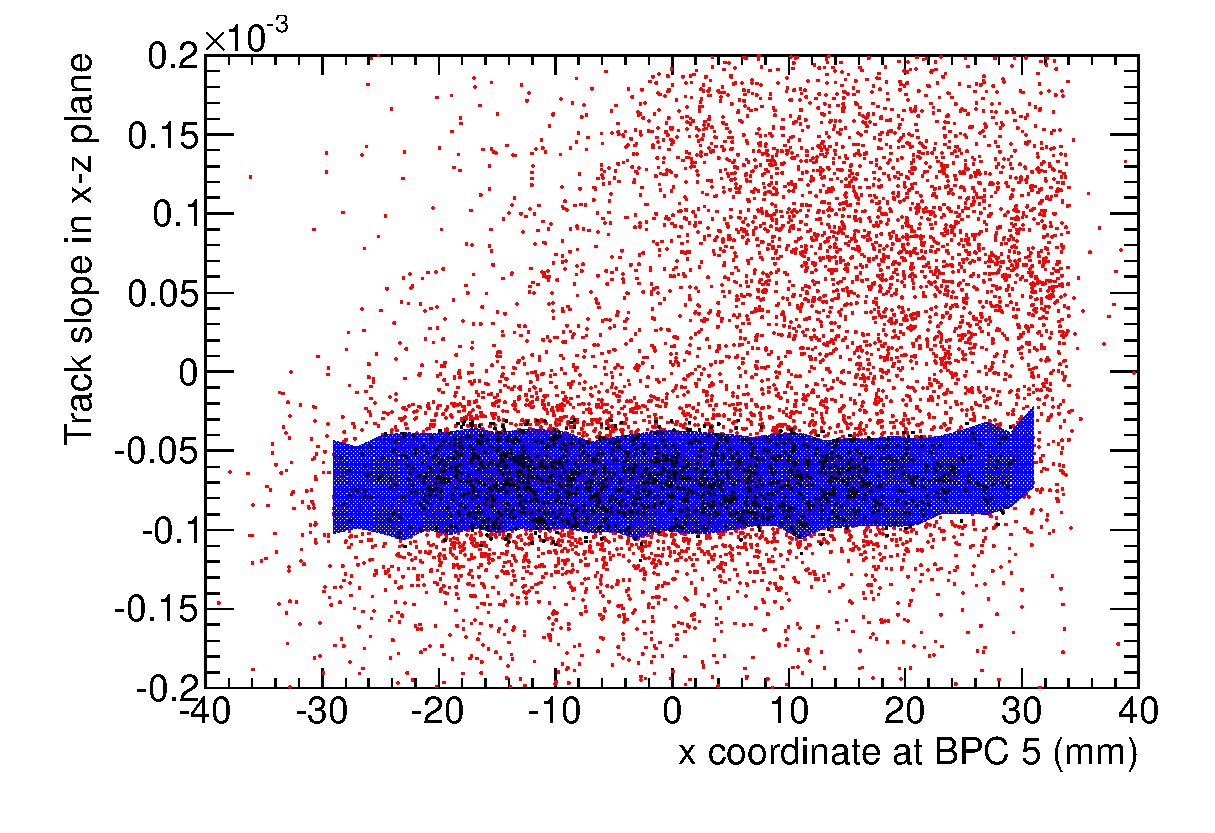
\includegraphics[width=0.45\linewidth,angle=0]{FCalTB_plots/tracks_x_e_run2324.eps}
\label{envelope_fig_x}
}
\subfigure{

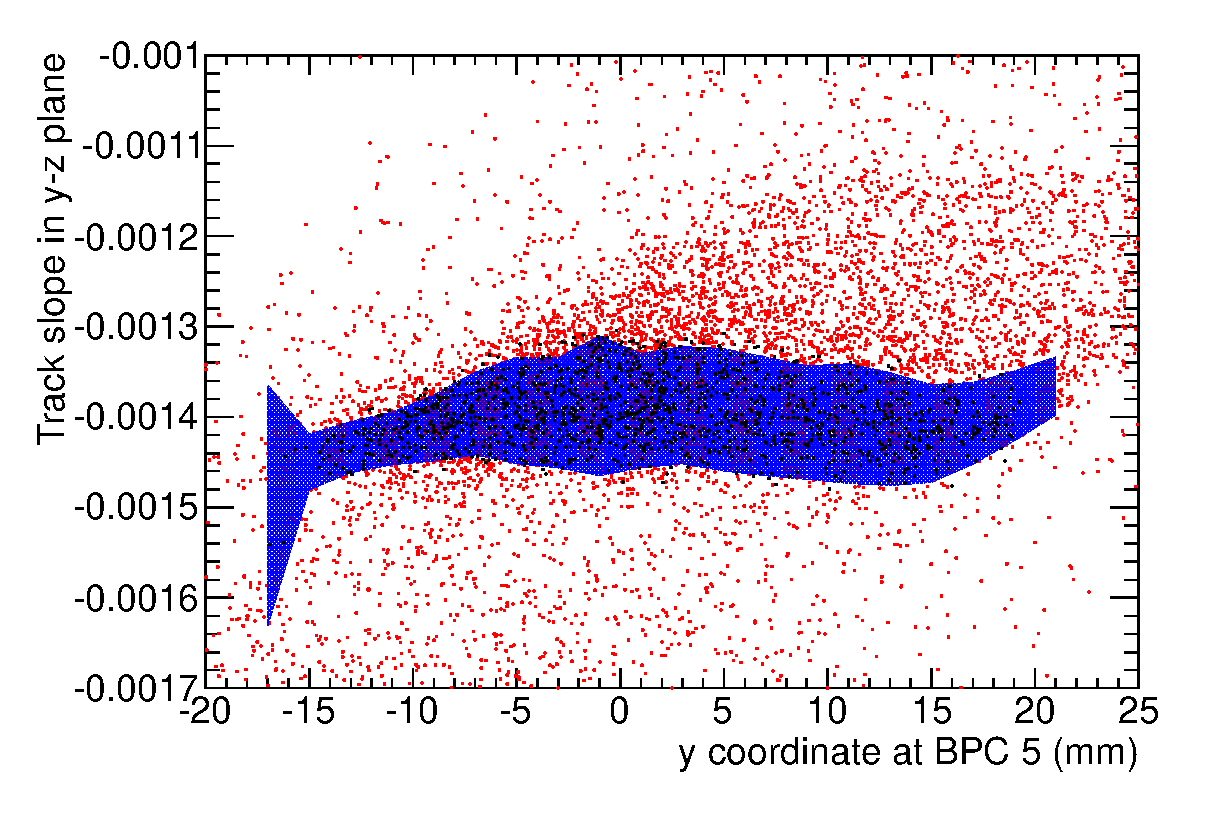
\includegraphics[width=0.45\linewidth,angle=0]{FCalTB_plots/tracks_y_e_run2324.eps}
\label{envelope_fig_y}
}
\caption{Particle trajectories in the $x-z$ plane (left) and the $y-z$ plane (right), taken from a 193 GeV electron run directed at position 4L. The region shaded in blue corresponds to the beam envelope, while the black (red) markers correspond to tracks that pass (fail) the envelope cut. Note that a track must lie within both envelopes in order to pass the beam envelope cut. } 
\label{envelope_fig}
\end{centering}
\end{figure}

%%%%%%%%%%%%%%%%%%%%%%%%%%%%%%%%%%%%%%%%%%%%%%%%%%%%%%%%%%%%%%%


As mentioned in section~\ref{sec_TBoverview_timing}, two TDCs were used to measure the time interval between the trigger signal and the clock pulse from the TTC, at which time the signals from the calorimeter were sampled. Output from the TDC is given as an integer number of TDC counts, between $\sim 300$ and $\sim 800$, which covers a time interval of 25 ns and thus gives the TDC a time resolution of 50 ps. There are three regions where a mismeasurement of the TDC can be problematic: near the TDC's minimum value, its maximum value, and in the ``wrap-around'' region. The wrap-around point is where the phase jump occurs, such that the time interval measured by the TDC jumps suddenly from 0 ns to 25 ns. The TDC phase quality is defined as the smallest difference between the TDC reading and one of the problematic regions. Event timing was determined using the TDC which had the highest phase quality. Events were rejected in cases where the readout from the highest quality TDC TDC was still within 1 ns of a problematic region.
% The event was rejected if the TDC phase quality did not lie in the range 20 $<$ TDcPhaseQuality $<$ 230, as in these cases the better clock choice was still within 1 ns of a problematic region.
%} %not stoked abouot this

%An additional timing cut was implemented using $\tau$, the time of the pulse peak as reconstructed by the OFCs (c.f. equation~\ref{eq_ofc_AT}. 
%
%
%halfling cut goes here.

The CEDAR detector (described in section~\ref{sec_TBoverview_beamline}) was also used to improve the beam purity. It was mainly used to eliminate proton events when analysing data taken with $\pi^+$ beams, by rejecting events containing beam particles that the CEDAR did not identify as charged pions. However, the CEDAR information was also used when recording electron data at 60~GeV, as the electron beams had a low purity at this energy.

%
%also another cut.
%
%The TDC Phase Quality is defined as the 
%
%
%
%Timing cut. 











%The measured slope is then compared to the ideal slope, and the procedure is repeated in the $y-z$ plane. For each direction, the difference between the ideal and measured track slopes in each direction are then summed in quadrature. and if the sum exceeds a specified threshold 
%
%it's chi^2 in track slope.
%
%The same thing is done in the $y$ direction, and in each case the deviation of the measured track from the ideal track is computed.  The difference between the actual track slope and the ideal track slope is then computed, and the process is repeated in the $y-z$ plane
%Beam envelope cuts? they work how?
%
%look at closest bpc to FCal
%if based on it's position, determine ideal slope for this intercept
%envelope of slopes determined around this. difference between actual slope and ideal slope determined. If the significance of this difference exceeds some threshold, event is cut.
%
%actual slope is "allowed" to be 
%
%
%Timing cuts.






%The BPCs were also 
%
%
%Beam cleaning
%- remove multiple particles and those that are scattered
%remove impurities from beam
%
%S1 S2 S3 signal over mip signal
%also BPCS - same deal
%
%
%
%CEDAR used on electron runs to remove pions, and on pi+ runs to remove protons.
%
%Beam envelope cuts - BPCS give good measurement of particle tracks - straight line fit to determine position and direction
%Cut if quality of fit is shit(?)
%Also used beam envelope. (Check this again) particles with different charge/mass ratios tend to occupy different regions of phase space in (x,v). Tracks are analysed, envelopes are defined for pions and electrons. Reject event if track isn't within envelope, or is too far outside it.
%
%
%
%timing - halflings?
%clustering timing cut.
%TBphase quality cut




\section{Cylindrical Cell Clustering}

\subsection{Analysis of Electron Data}

%events taken with electron and positron beam, polarity determined by other experiments
%
%no. of triggers?
%
%final events after all cuts
%
%response plotted goes here

%\red{fancy timing cut should go somewhere}









%
%What is the deal with the beam polarity, exactly. 
%
%cuts used as described earlier. CEDAR is off, except at 60~GeV where its hard to get a good, pure beam.

Using the tracking information obtained from the BPCs, the point at which the beam particles strike the front face of the calorimeter can be determined. Cylindrical clusters are then formed by collecting all cells within a certain distance of the impact point. For the analysis of data taken with electron beams, only calorimeter cells in FCal1 are considered. For the analysis of data taken with pion beams, calorimeter cells from all three FCal modules are included in the cylindrical cluster. As the FCal was oriented at an angle with respect to the incoming beam particles, the beam particle track is projected through the FCal to give a slightly different impact point for each module. In the calorimeter coordinate system, the impact point changes by $~\sim 2cm$ between neighbouring modules.

%Cylindrical clusters are then formed by summing the energy of each cell within a certain radius of this impact point. A clustering radius of 8 cm is used for analysis of the electron data. 
%
%
%The moliere radius is a quantity used to describe the transverse development of electromagnetic showers. It is given by \blue{blah}, and on average $\sim 90\%$ of the shower energy is contained witihin a cylinder of radius $\sim R_M$. \cmt{can cite paper on my desk by fabiola and fabjen, calorimetery in particle physics, reviews of modern physics}.
%either do this here or in detector chapter, where moliere is first mentioned
%
%

On average, about 90\% of the energy deposited by an electromagnetic shower is contained within a cylinder of radius $\rho_M$, the \moliere radius \cite{fabiola_calorimetry}. In FCal1 the \moliere radius is 17mm, and $\sim 99\%$ of the energy is contained within a cylindrical cluster of radius 8cm, as can be seen in Figure~\ref{TBplot_electron_radials}. Clusters with radii 12 cm and 16 cm are also generated during event reconstruction. These larger clusters capture about 1\% more energy than the 8 cm cluster, however the noise contained within the cluster increases by $\sim50 \%$ at a radius of 12 cm and  $\sim100 \%$ at a radius of 16 cm. For this reason 8 cm clusters are used in the analysis of electron data. 



%%%%%%%%%%%%%%%%%%%%%%%%%%%%%%%%%%%%%%%%%%%%%%%%%%%%%%%%%%%%%%%
\begin{figure}[!htbp]
\begin{centering}
\subfigure{
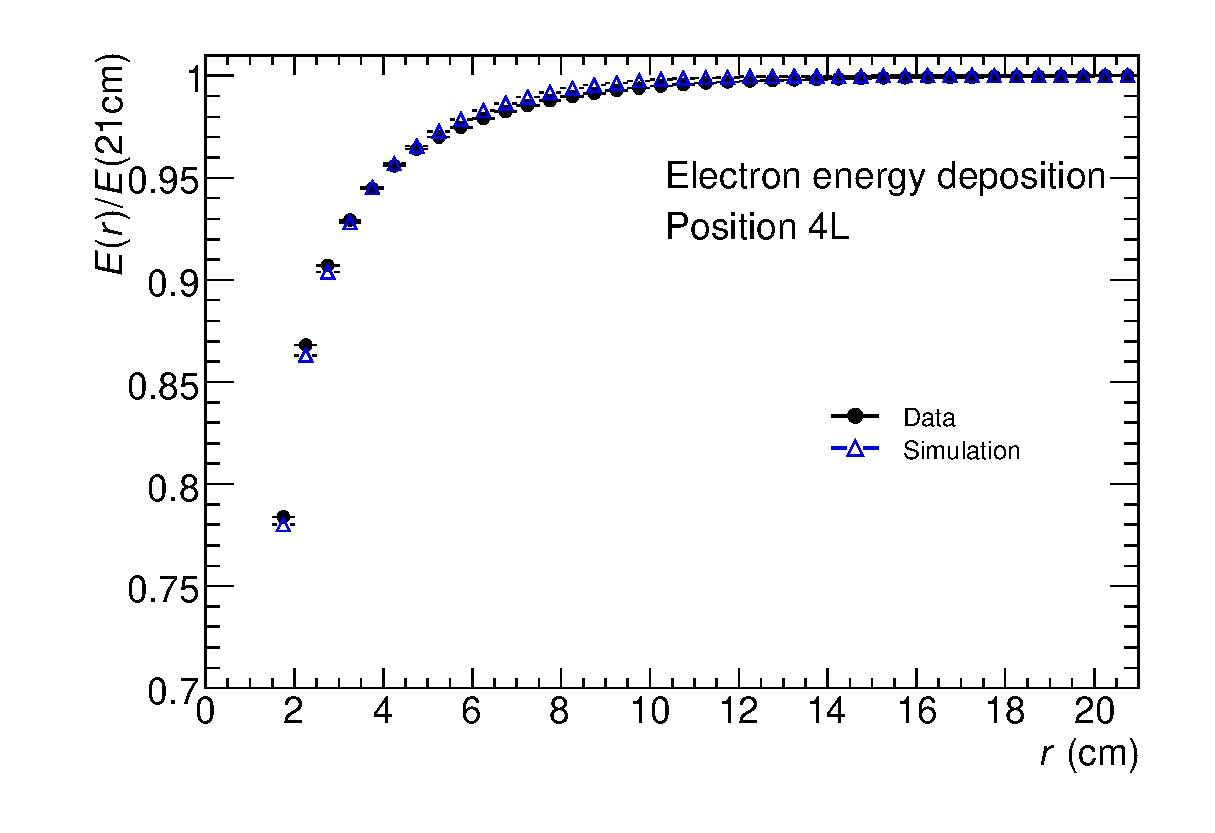
\includegraphics[width=0.45\linewidth,angle=0]{FCalTB_plots/radial_electrons_4L_193GeV_int.eps}
\label{TBplot_electron_rad_4L_int}
}
\subfigure{

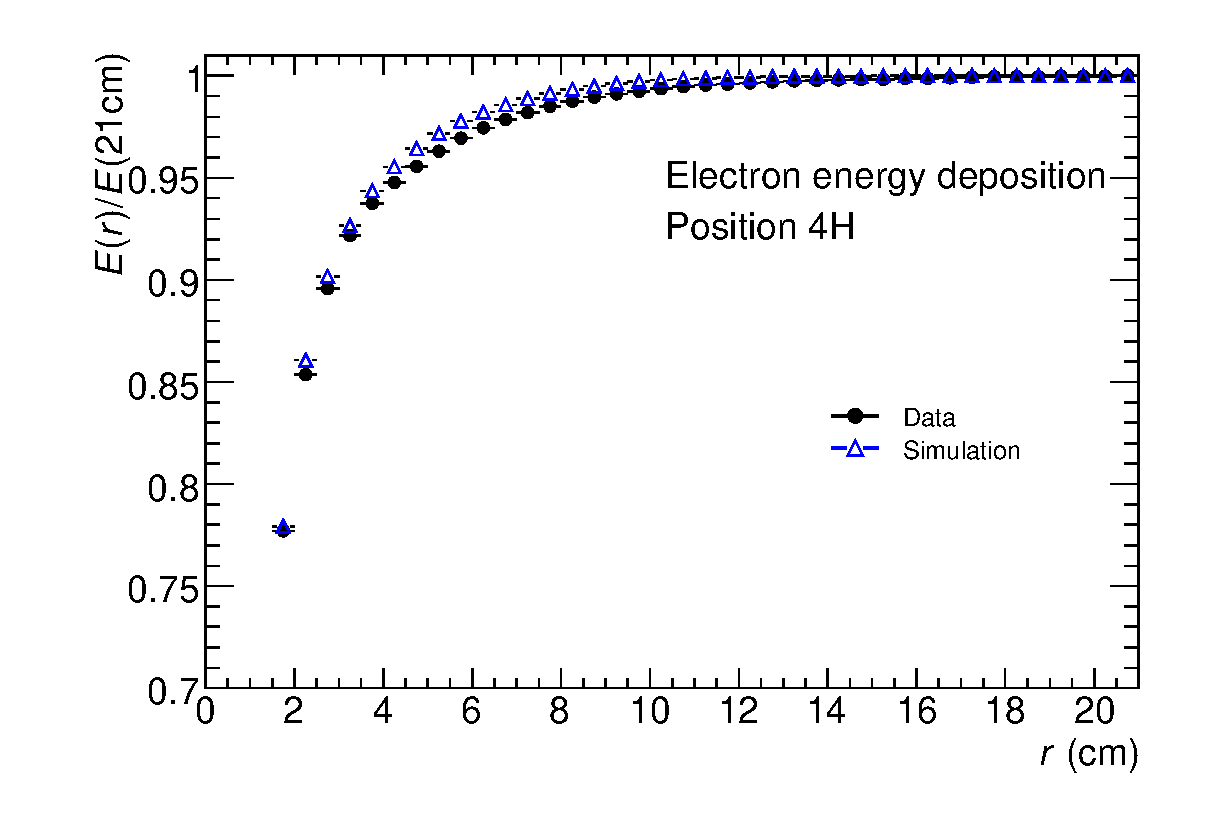
\includegraphics[width=0.45\linewidth,angle=0]{FCalTB_plots/radial_electrons_4H_193GeV_int.eps}
\label{TBplot_electron_rad_4H_int}
}\\
\subfigure{
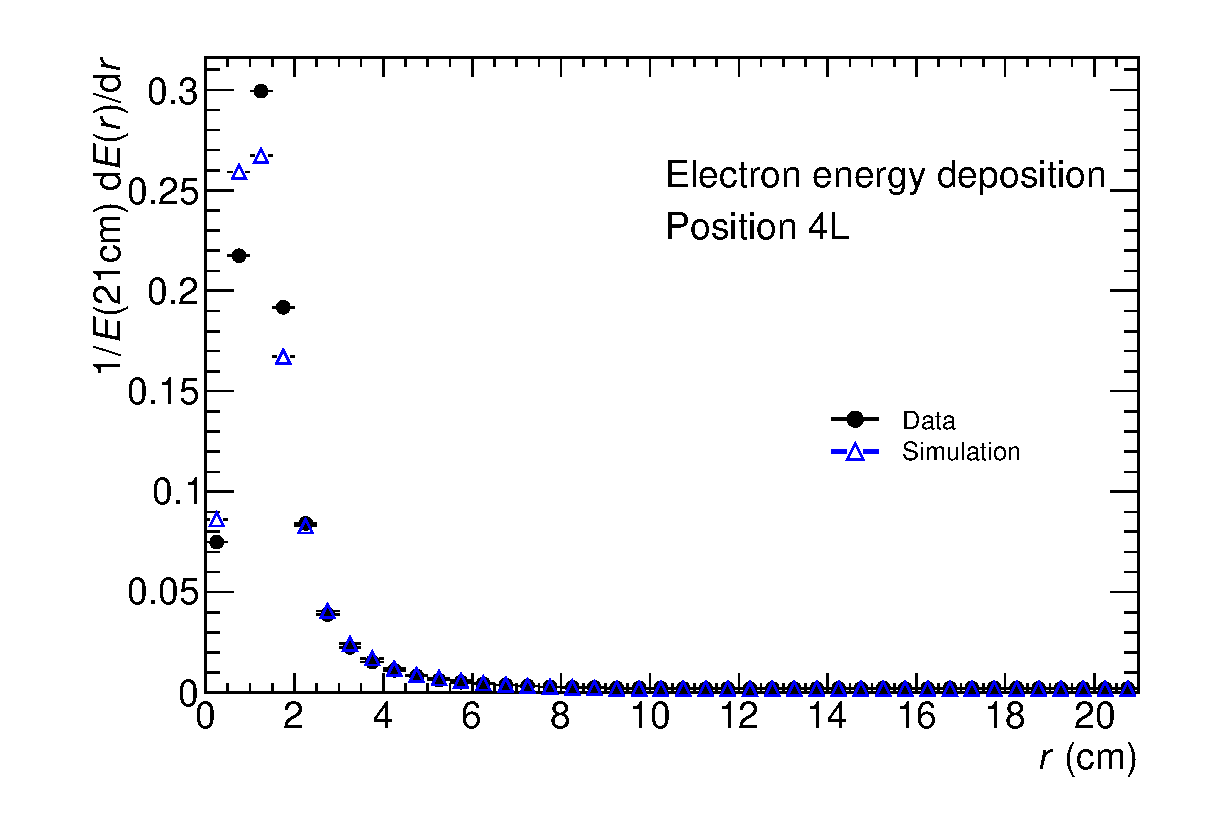
\includegraphics[width=0.45\linewidth,angle=0]{FCalTB_plots/radial_electrons_4L_193GeV_diff.eps}
\label{TBplot_electron_rad_4L_diff}
}
\subfigure{

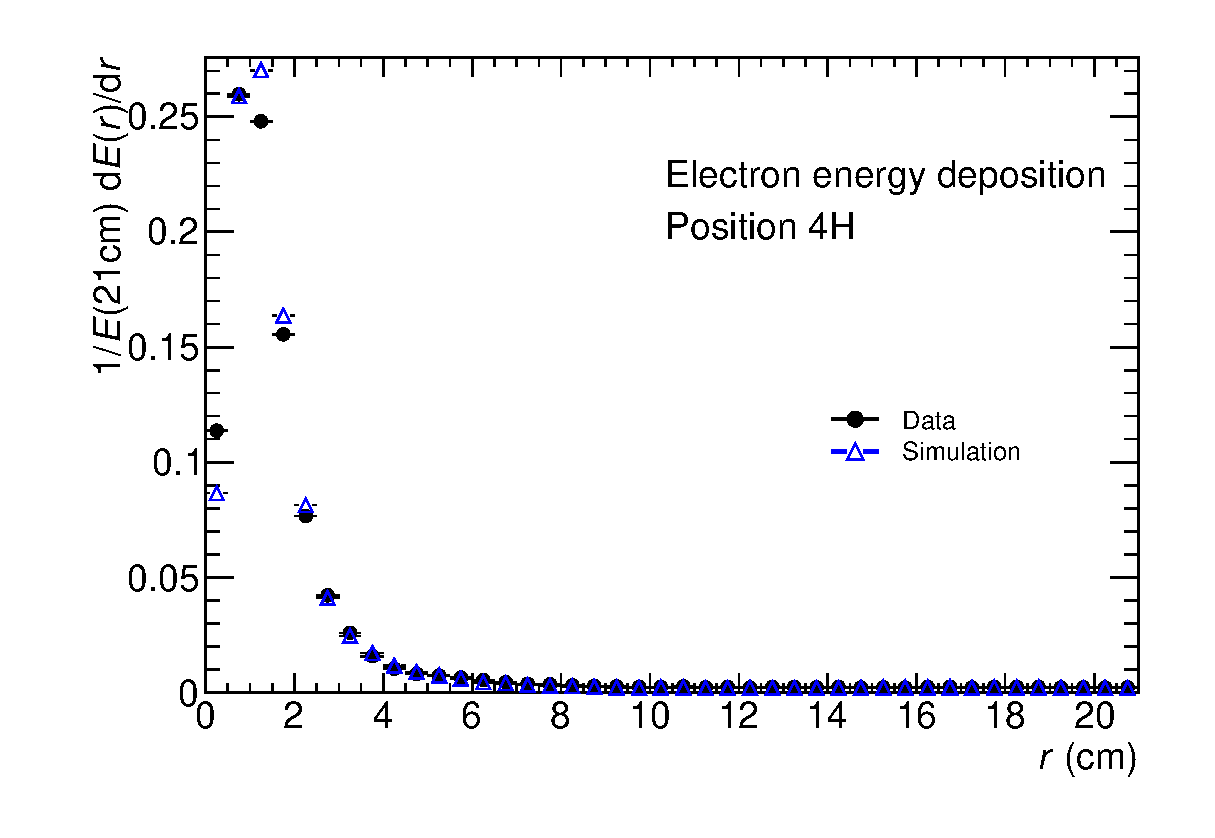
\includegraphics[width=0.45\linewidth,angle=0]{FCalTB_plots/radial_electrons_4H_193GeV_diff.eps}
\label{TBplot_electron_rad_4H_diff}
}
\caption{Energy contained in cylindrical clusters as a function of the clustering radius. Figures~\ref{TBplot_electron_rad_4L_int} and \ref{TBplot_electron_rad_4H_int} show the fraction of energy contained within a cylindrical cluster of radius $r$ compared to cluster of radius 21cm, for showers initiated by 193.1~GeV electrons at position 4L and 4H, respectively. Figures~\ref{TBplot_electron_rad_4L_diff} and \ref{TBplot_electron_rad_4H_diff} show the fractional energy deposited between $r$ and $r+\ud r$ as a function of $r$, for position 4L and 4H respectively.} 
\label{TBplot_electron_radials}
\end{centering}
\end{figure}

%%%%%%%%%%%%%%%%%%%%%%%%%%%%%%%%%%%%%%%%%%%%%%%%%%%%%%%%%%%%%%%



%\red{halflings}

%. The BPCs present in the beamline are used to obtain the trajectory of the beam particle, which is then projected to a point on the front face of the FCal1 module. A cluster is then created by summing the energy of all FCal1 channels within 8cm of the impact point. 

The energy reconstructed for a given particle is dependent on the position at which that particle impacts the calorimeter, as an electron striking the centre of an electrode rod deposits less visible energy in the calorimeter than one that impacts close to the liquid argon gap \cite{TB98_electron_signals}. As the diameter of the beamspot (65 mm) is an order of magnitude larger than the spacing between adjacent electrodes (7.5 mm in FCal1), many different impact points are sampled. This leads to a non-Gaussian distribution in the response, as the response is essentially the sum of many different Gaussian distributions. A good fit to the data is obtained using a double Gaussian function,

\begin{equation}
F(E) = a_0 \exp \left( - \frac{(E - a_1)^2}{2 a_2^2} \right ) +  a_3 \exp \left( - \frac{(E - a_4)^2}{2 a_5^2} \right)
\label{eqn_dbl_Gaussian}
\end{equation}
%where $A_i$, $\mu_i$, and $\sigma_i$ are the peaks, means and widths of the component Gaussians. The mean response is then found by taking the first moment of $F(E)$, such that
where the parameters $a_0$ and $a_3$ describe the amplitudes, $a_1$ and $a_4$ describe the means, and $a_2$ and $a_5$ describe the widths of the component Gaussians. 
%$A_i$, $m_i$, and $\sigma_i$ are the amplitudes, means and widths of the component Gaussians, respectively. 
When fitting the response distributions with the double Gaussian, some constraints are imposed on the parameters. The non-Gaussian shape of the response is determined by the geometry of the calorimeter, as this determines which impact points are closer to a liquid argon gap (yielding a higher reponse), and which impact points are further from the gap (giving a lower response). This suggests that the shape of the response should be independent of the beam energy, which allows some constraints to be imposed on the fit parameters in equation~\ref{eqn_dbl_Gaussian}. The ratio of the populations and the means of the two Gaussians are held fixed, such that
\begin{eqnarray}
\frac{a_0 a_2}{a_3 a_5} & = & C_1 \label{eqn_constraint_1}\\
\frac{a_1}{a_4} & = & C_2,
\label{eqn_constraint_2}
\end{eqnarray}
where $C_1$ and $C_2$ are constants. These constants are determined by performing an unconstrained double Gaussian fit on the 193 GeV electron data (or 200~GeV hadron data). The values obtained from this unconstrained fit are then used to apply constrained fits to the responses at lower beam energies.
%
%variation in impact point
%variation in response
%due to geometry
%
%two Gaussians used to fit this response
%
%relative populations and means therefore determined by geometry
%independent of energy/constrained.
%
%
%
%
%
%As the variation in the response is due to variations in the beam particle impact point,  These constraints are motivated by the geometry of the calorimeter: as this is responsible for the
%

The mean response, $\overline{E}$, is taken as the first moment of $F(E)$, where the $i$-th moment, $\mu_i$, is given by
\begin{equation}
\label{eqn_moment}
\mu_i = \frac{\int^{E_{\mathrm{max}}}_{E_{\mathrm{min}}}  E^{i} F(E) \ud E }{\int^{E_{\mathrm{max}}}_{E_{\mathrm{min}}}  F(E) \ud E},
\end{equation}
where the limits of the integral, $E_\mathrm{min}$ and $E_\mathrm{max}$, are obtained from the response histogram. The lower limit, $E_\mathrm{min}$, is taken from the low edge of the lowest energy bin that is not empty, while $E_\mathrm{max}$ is the upper edge of the highest non-empty histogram bin. 

The width of the response, $\sigma$, is determined from the first and second moments of $F(E)$, such that
%\begin{equation}
%\mu_2 = \frac{\int^{E_{\mathrm{max}}}_{E_{\mathrm{min}}}  E^2 F(E) \ud E }{\frac{\int^{E_{\mathrm{max}}}_{E_{\mathrm{min}}}  F(E) \ud E},
%\end{equation}
%such that
\begin{equation}
\sigma = \left( \mu_2 - \mu_1^2 \right)^{1/2}.
\label{DG_width_def}
\end{equation}

Statistical uncertainties on these quantities may be written in terms of higher order moments. For simplicity, a (single) Gaussian fit is made to the response, and the moments of this Gaussian are used to compute the statistical uncertainties. The statistical uncertainties on $\overline{E}$ and $\sigma$ are then
\begin{eqnarray}
\Delta \overline{E} = \Delta \mu_1 & = & \frac{\sigma_g}{\sqrt{N_g}} \\
\Delta \sigma & = & \frac{\sigma_g}{\sqrt{2N_g}},
\end{eqnarray}
where $\sigma_g$ and $N_g$ are the width and population of the (single) Gaussian fit.




The response of the FCal to electron beams is plotted in Figures~\ref{TBplot_electron_response_4L_data} and \ref{TBplot_electron_response_4H_data}, for beams directed at positions 4L and 4H, respectively. These results are summarized in Tables \ref{TBres_table_elec_4L} and \ref{TBres_table_elec_4H}. 
%%%%%%%%%%%%%%%%%%%%%%%%%%%%%%%%%%%%%%%%%%%%%%%%%%%%%%%%%%%%%%%
\begin{figure}[p]
\begin{center}
\subfigure{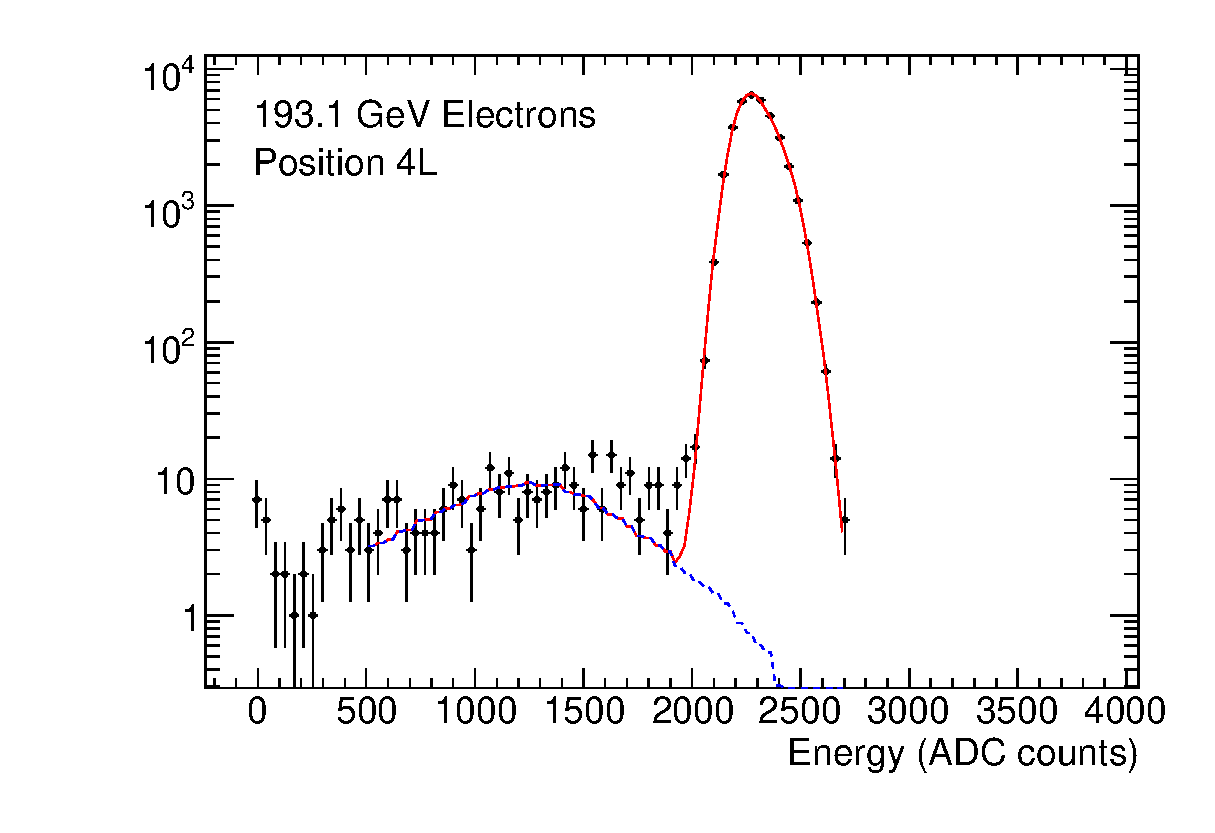
\includegraphics[width=0.45\linewidth,angle=0]{FCalTB_plots/Response_individual_data/Electron_response_193GeV_4L_data.eps}}
\subfigure{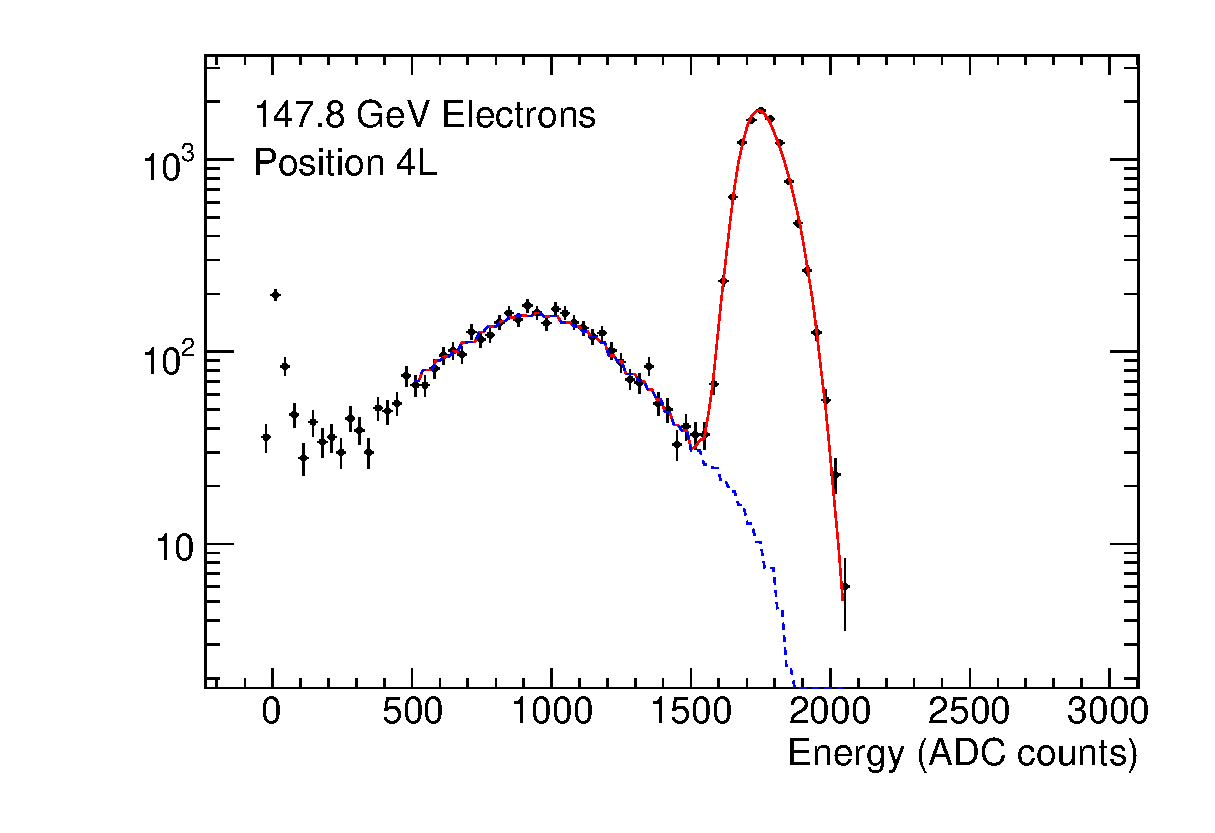
\includegraphics[width=0.45\linewidth,angle=0]{FCalTB_plots/Response_individual_data/Electron_response_148GeV_4L_data.eps}}\\
\subfigure{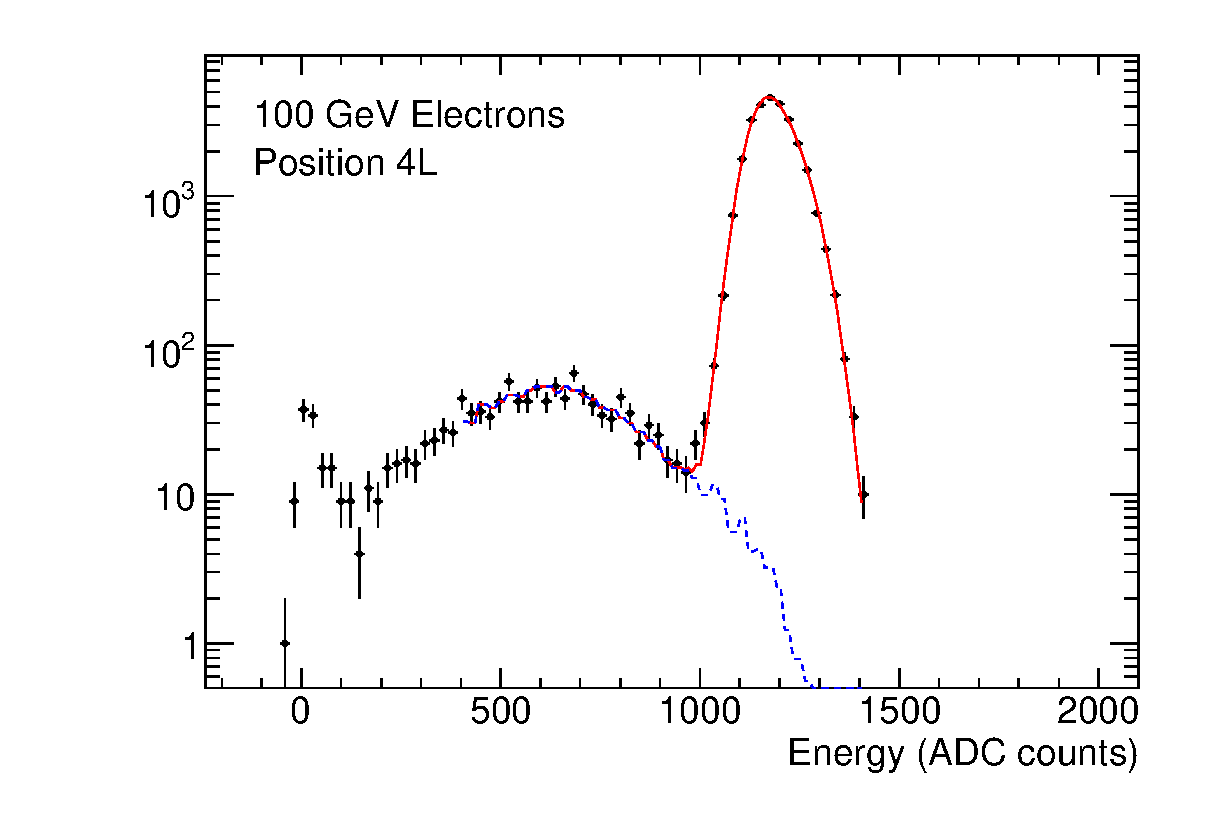
\includegraphics[width=0.45\linewidth,angle=0]{FCalTB_plots/Response_individual_data/Electron_response_100GeV_4L_data.eps}}
\subfigure{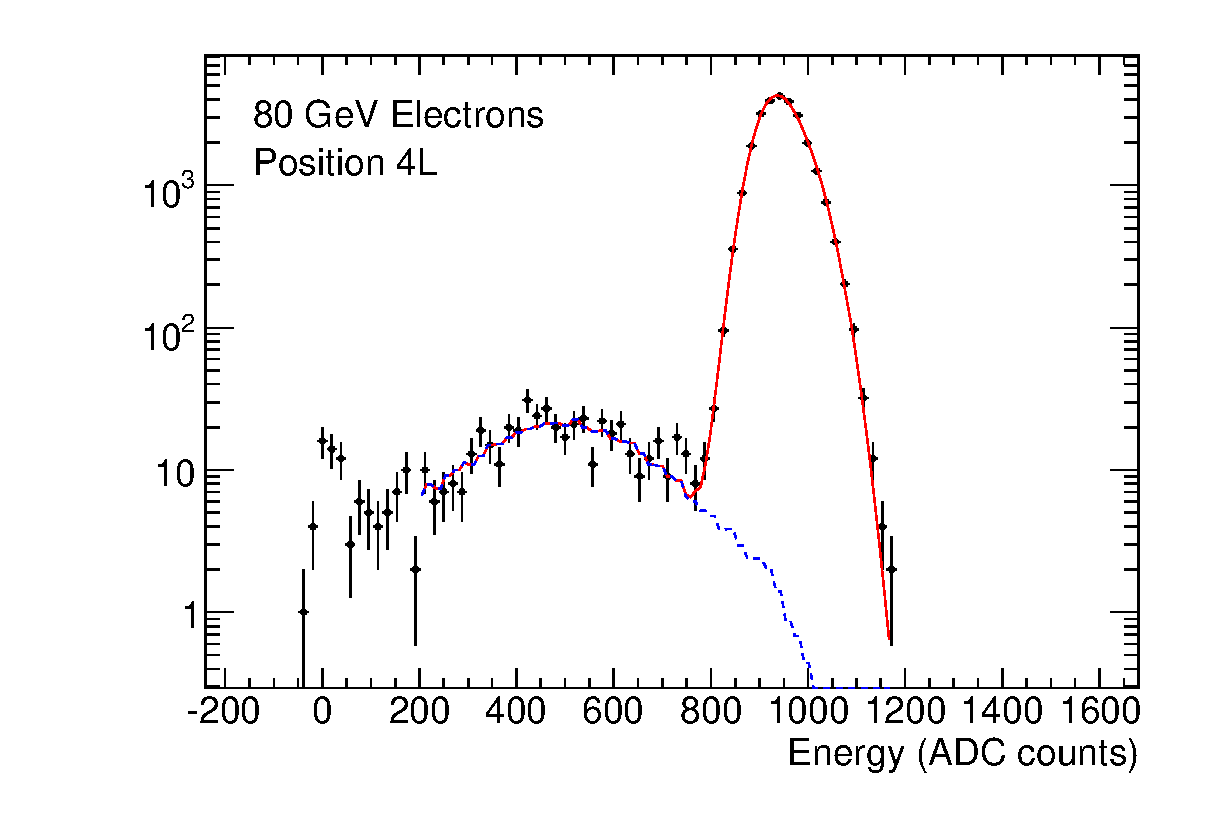
\includegraphics[width=0.45\linewidth,angle=0]{FCalTB_plots/Response_individual_data/Electron_response_80GeV_4L_data.eps}}\\
\subfigure{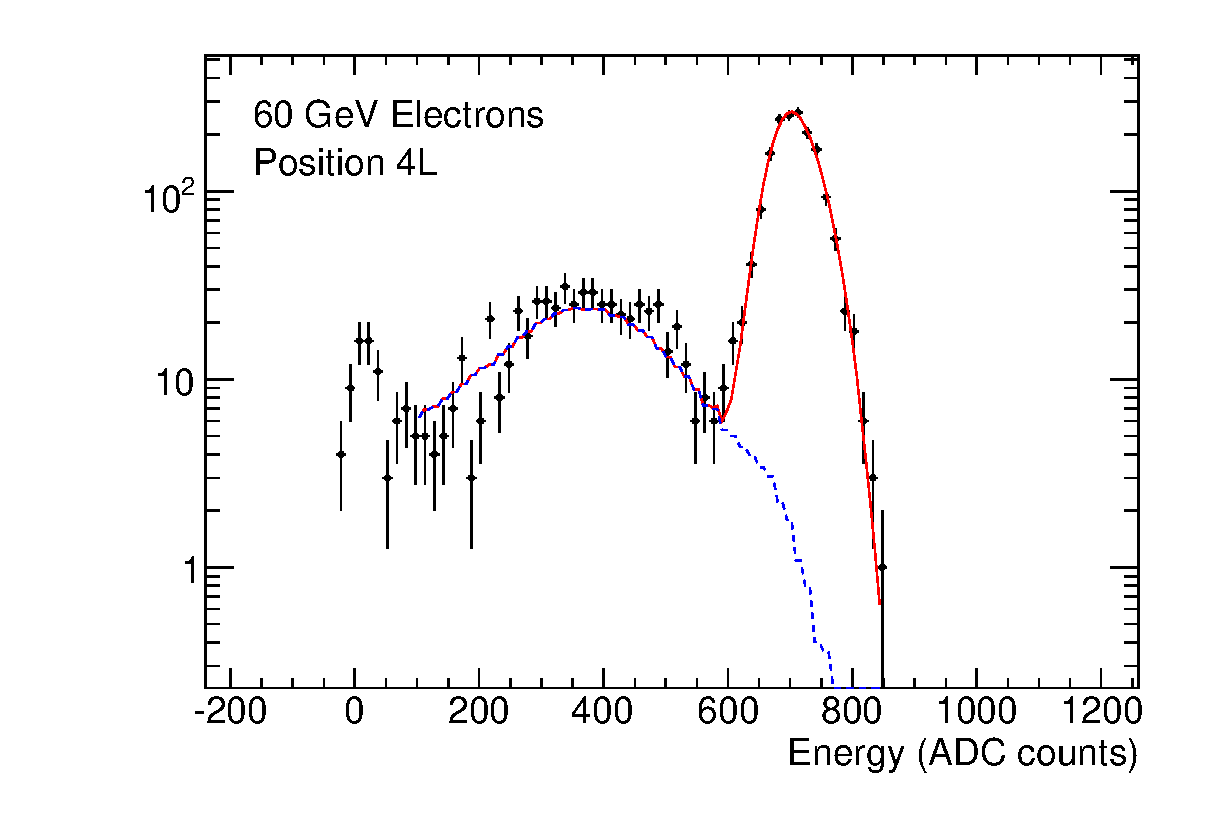
\includegraphics[width=0.45\linewidth,angle=0]{FCalTB_plots/Response_individual_data/Electron_response_60GeV_4L_data.eps}}
\subfigure{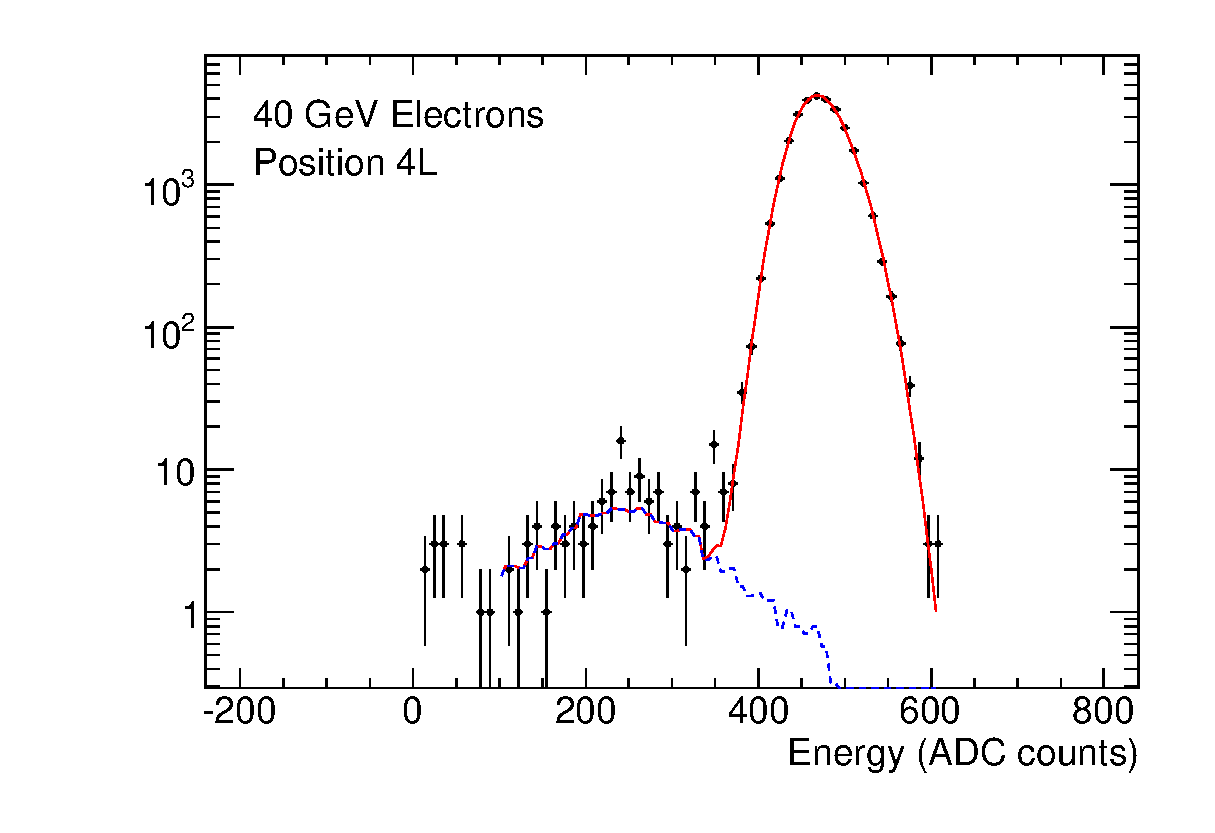
\includegraphics[width=0.45\linewidth,angle=0]{FCalTB_plots/Response_individual_data/Electron_response_40GeV_4L_data.eps}}\\
\subfigure{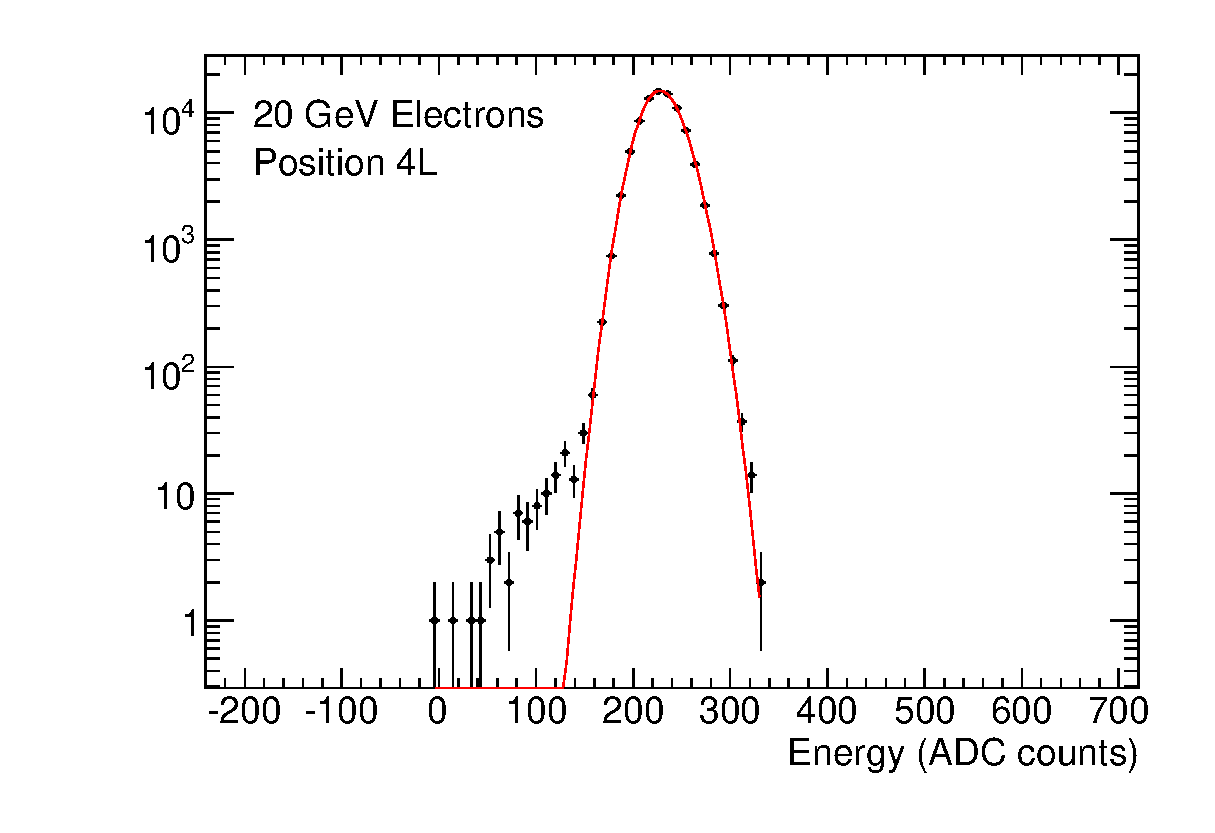
\includegraphics[width=0.45\linewidth,angle=0]{FCalTB_plots/Response_individual_data/Electron_response_20GeV_4L_data.eps}}
\subfigure{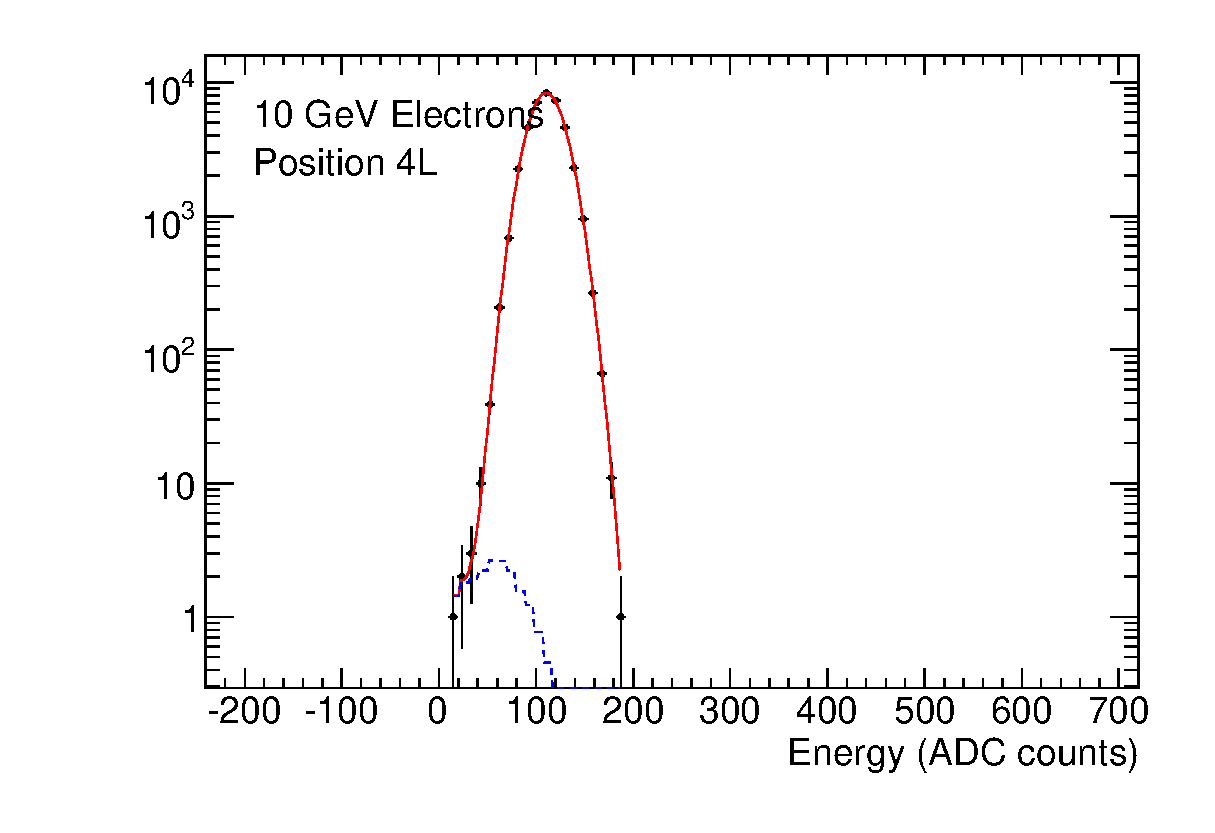
\includegraphics[width=0.45\linewidth,angle=0]{FCalTB_plots/Response_individual_data/Electron_response_10GeV_4L_data.eps}}
\end{center}
\caption{Response of the FCal to electrons directed at position 4L. The blue dashed curve shows the fit to the hadron contamination present in the data sample. The red curve is the total fit to the data, which consists of a double Gaussian fit to the electron peak as well as the fit to the hadron contribution.}
\label{TBplot_electron_response_4L_data}
\end{figure}






%%%%%%%%%%%%%%%%%%%%%%%%%%%%%%%%%%%%%%%%%%%%%%%%%%%%%%%%%%%%%%%

%%%%%%%%%%%%%%%%%%%%%%%%%%%%%%%%%%%%%%%%%%%%%%%%%%%%%%%%%%%%%%%

%\begin{figure}[!htb]
%\begin{center}
%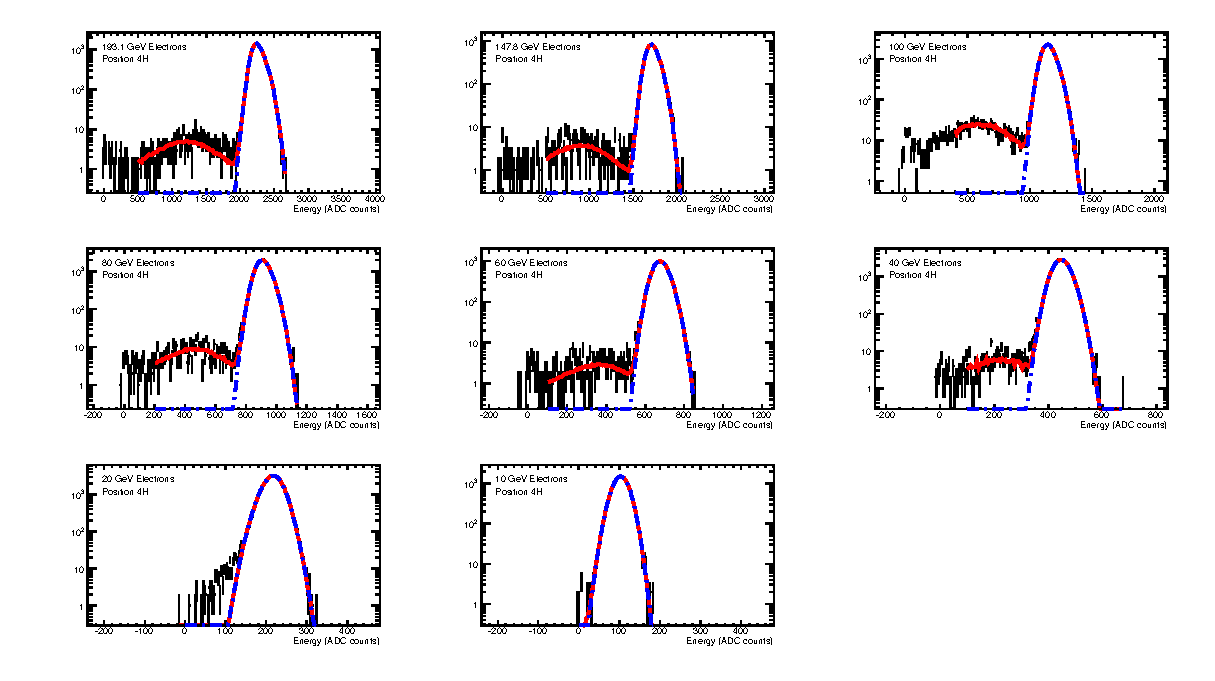
\includegraphics[width=1.0\linewidth,angle=0]{FCalTB_plots/electron_response_4H_data.eps}
%\end{center}
%\caption{Response of the FCal to electron beams directed at position 4H. The blue dashed curve double Gaussian fit to the electron peak, while the red curve shows the total fit to the electron peak plus the contaminant hadron contribution.}
%\label{TBplot_electron_response_4H_data}
%\end{figure}
%%%%%%%%%%%%%%%%%%%%%%%%%%%%%%%%%%%%%%%%%%%%%%%%%%%%%%%%%%%%%%%%
\begin{figure}[p]
\begin{center}
\subfigure{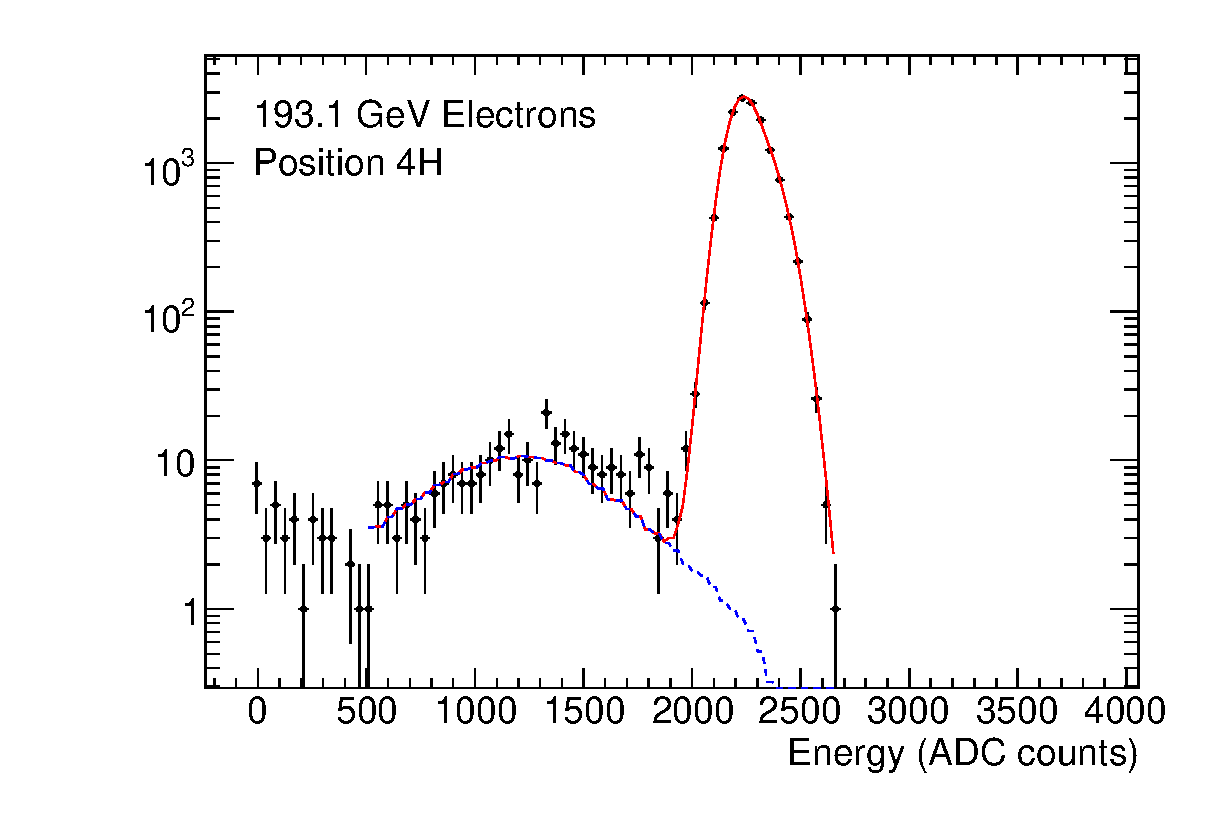
\includegraphics[width=0.45\linewidth,angle=0]{FCalTB_plots/Response_individual_data/Electron_response_193GeV_4H_data.eps}}
\subfigure{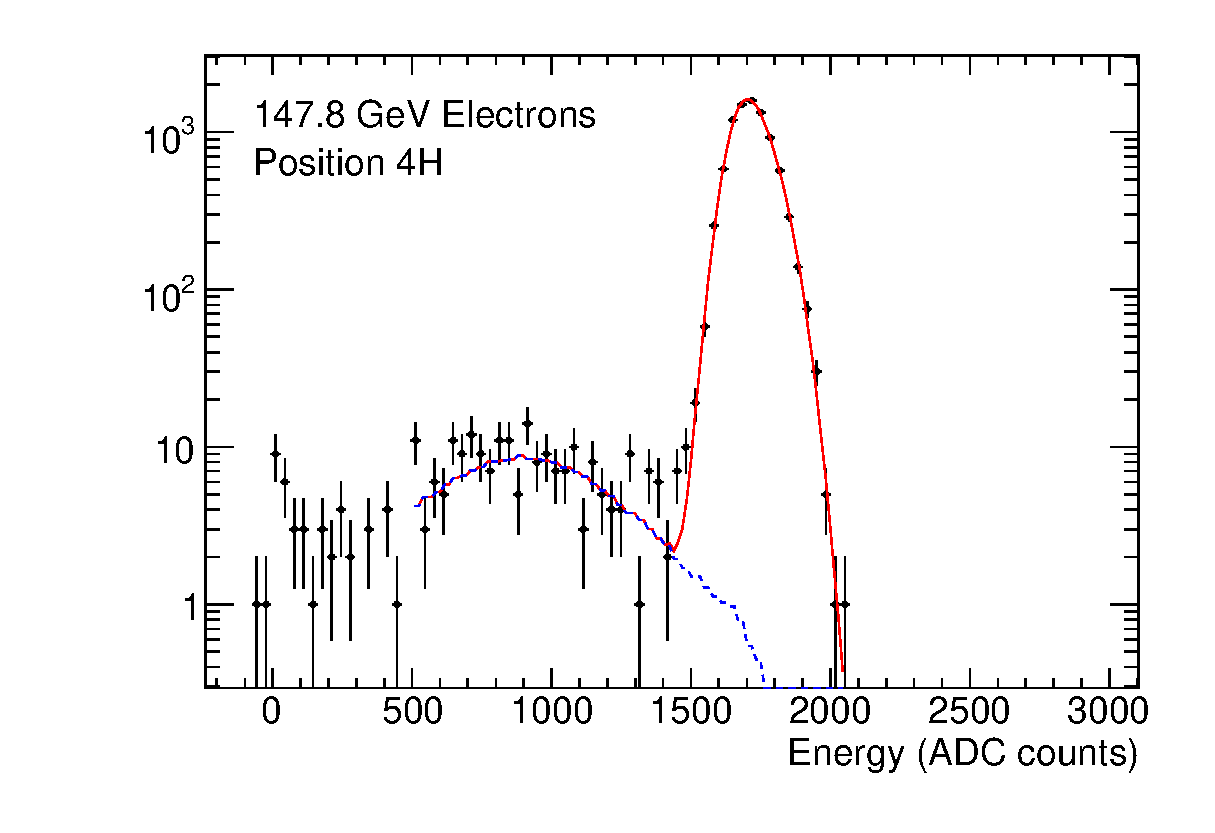
\includegraphics[width=0.45\linewidth,angle=0]{FCalTB_plots/Response_individual_data/Electron_response_148GeV_4H_data.eps}}\\
\subfigure{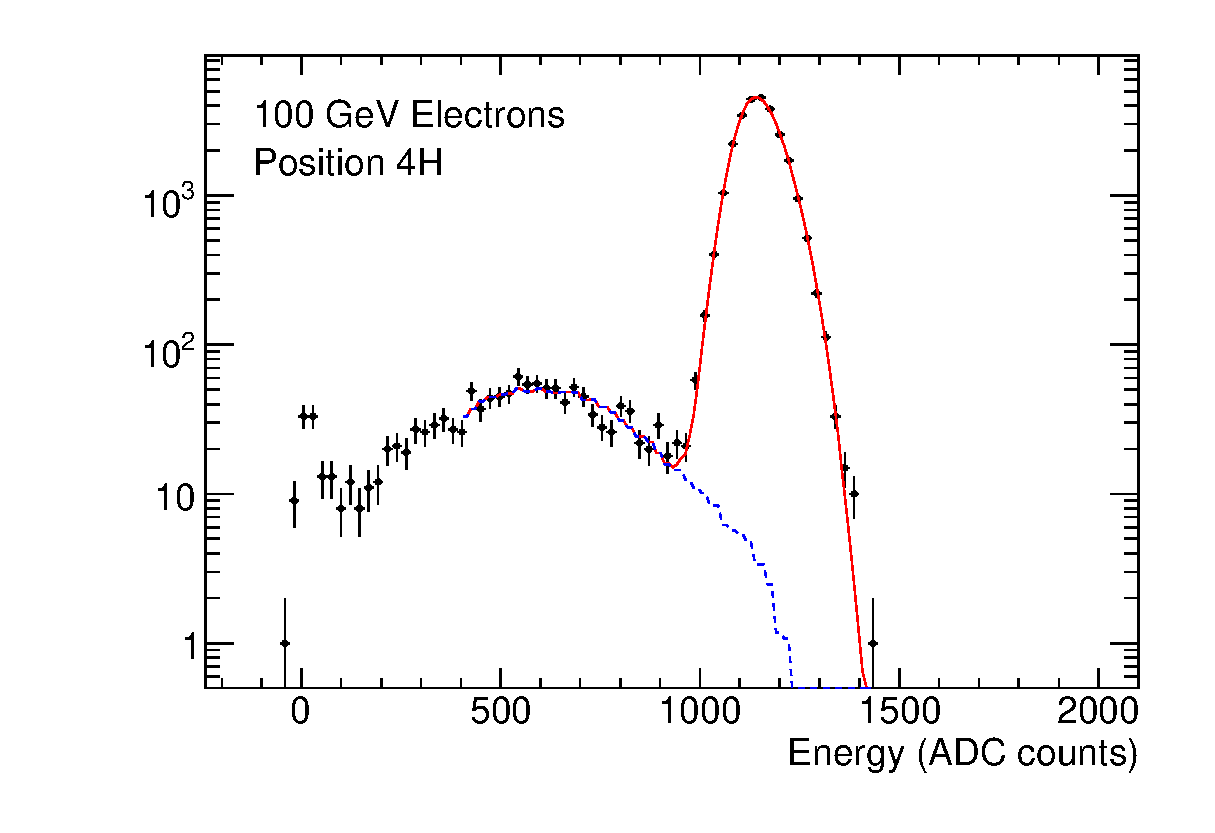
\includegraphics[width=0.45\linewidth,angle=0]{FCalTB_plots/Response_individual_data/Electron_response_100GeV_4H_data.eps}}
\subfigure{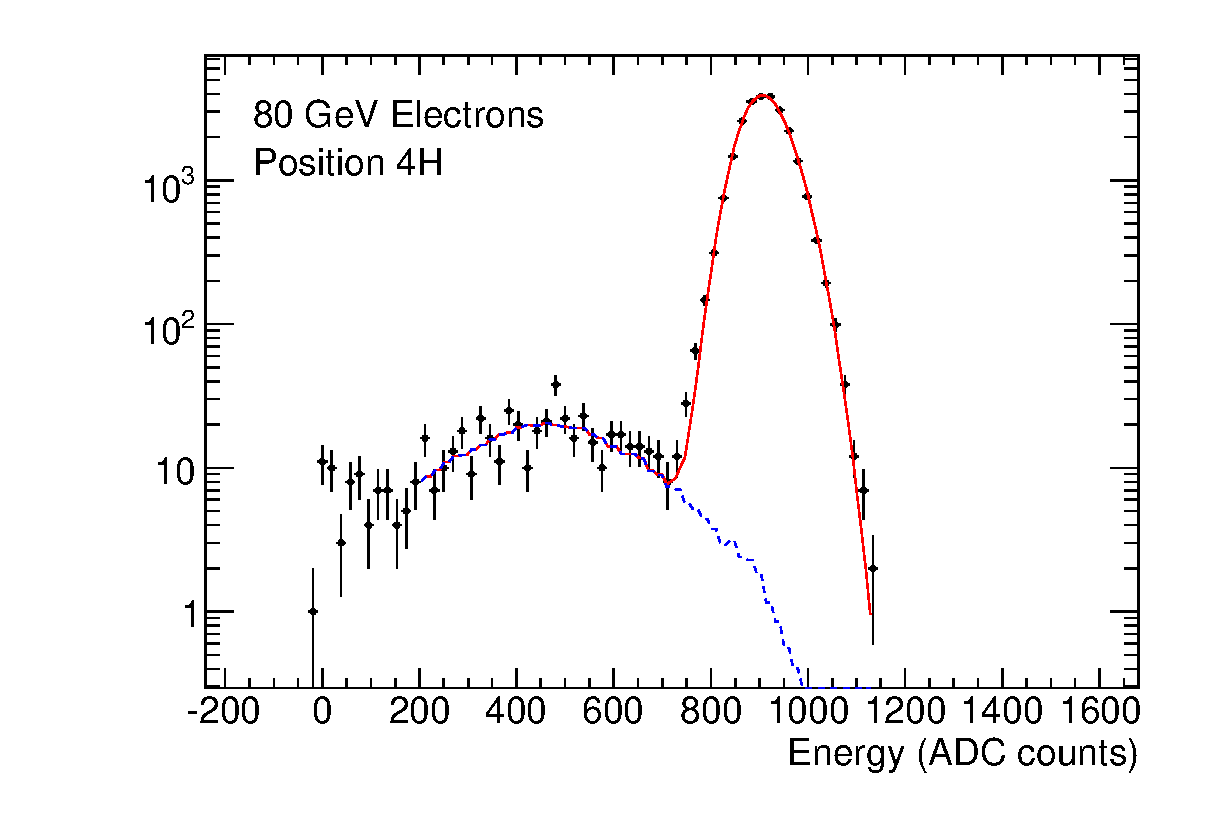
\includegraphics[width=0.45\linewidth,angle=0]{FCalTB_plots/Response_individual_data/Electron_response_80GeV_4H_data.eps}}\\
\subfigure{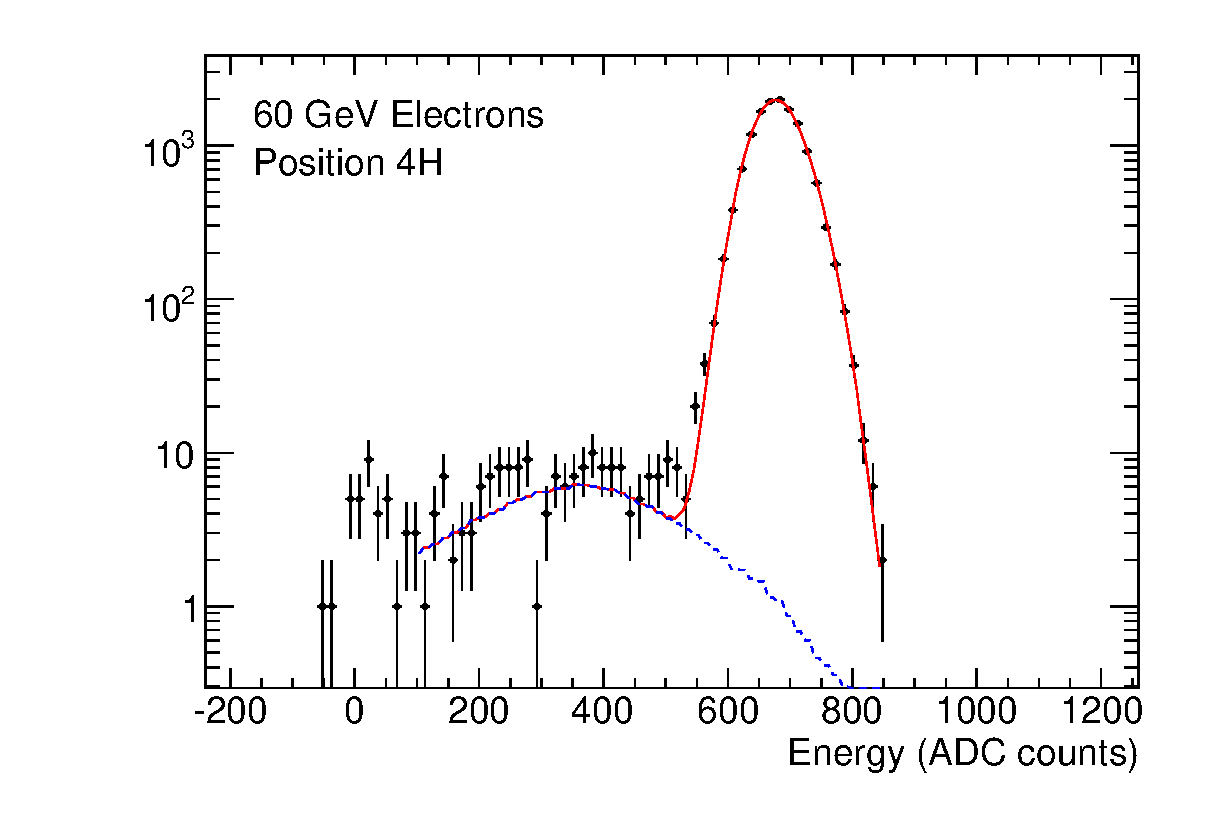
\includegraphics[width=0.45\linewidth,angle=0]{FCalTB_plots/Response_individual_data/Electron_response_60GeV_4H_data.eps}}
\subfigure{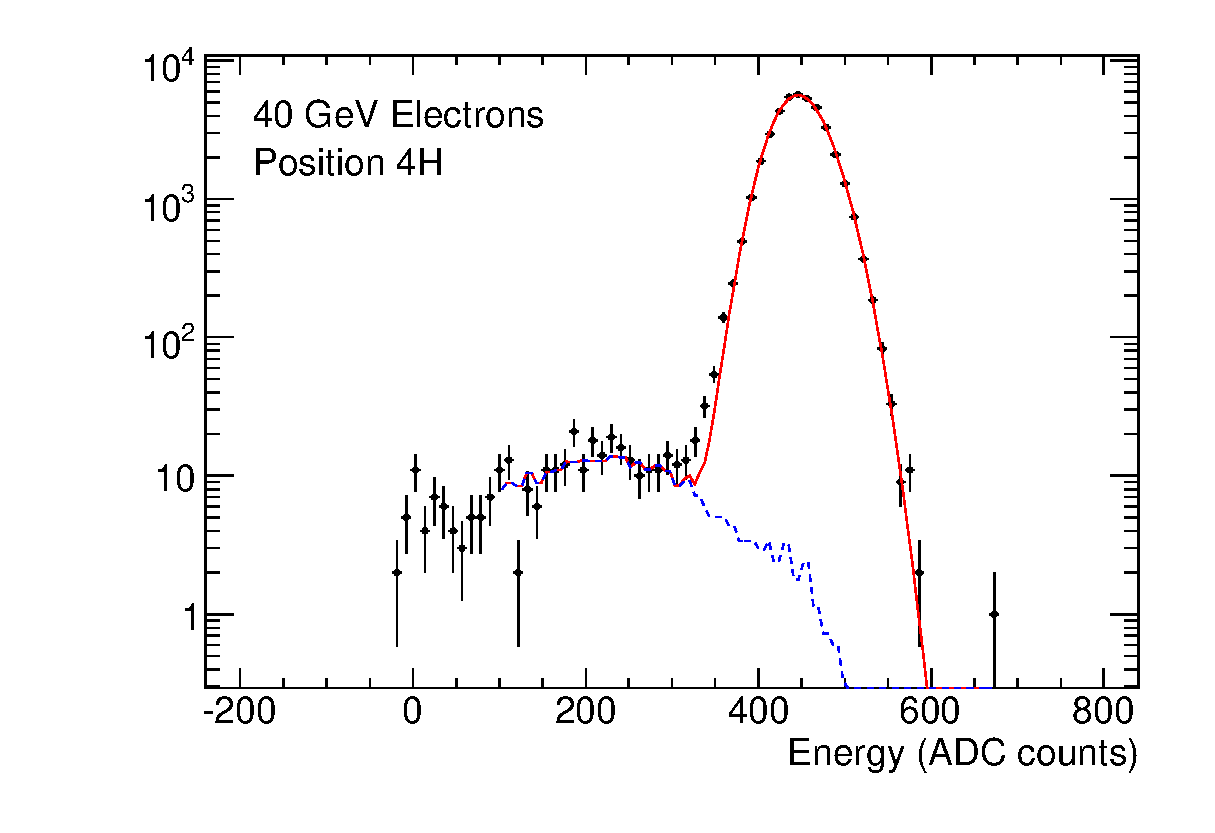
\includegraphics[width=0.45\linewidth,angle=0]{FCalTB_plots/Response_individual_data/Electron_response_40GeV_4H_data.eps}}\\
\subfigure{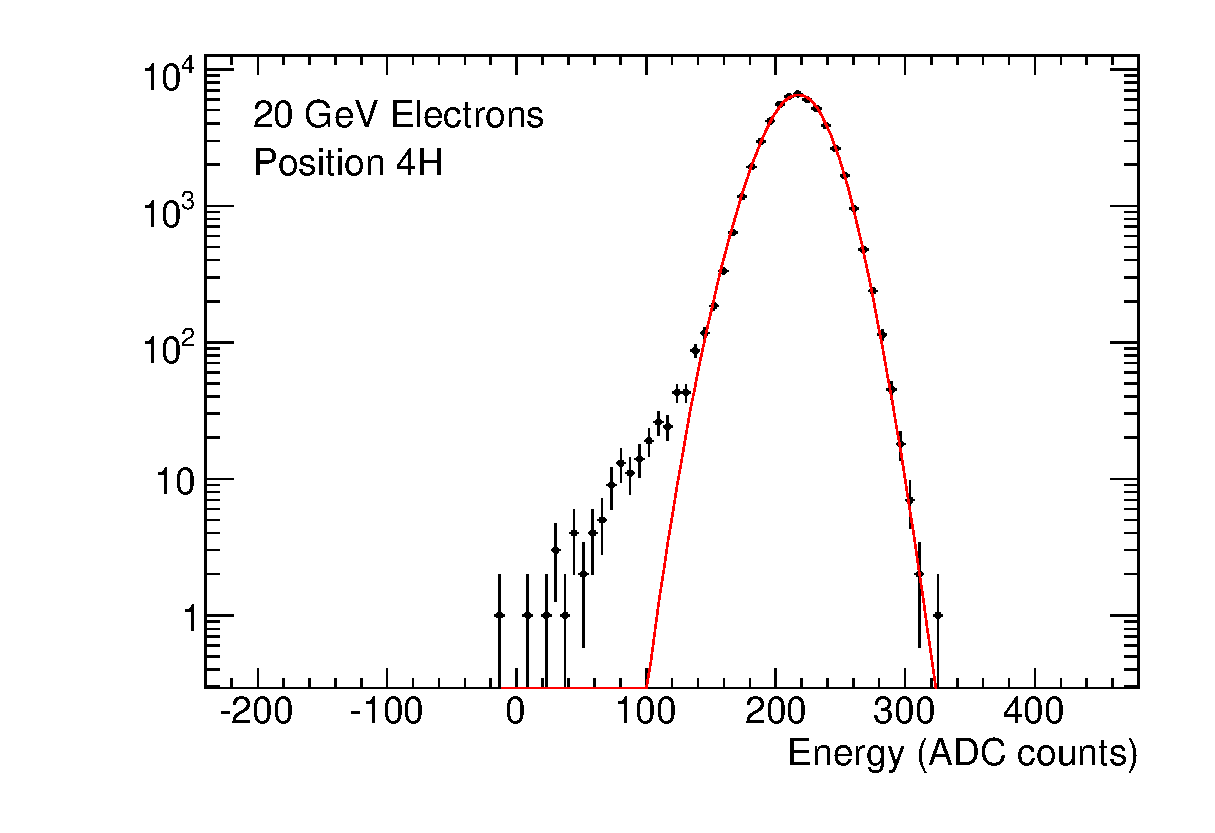
\includegraphics[width=0.45\linewidth,angle=0]{FCalTB_plots/Response_individual_data/Electron_response_20GeV_4H_data.eps}}
\subfigure{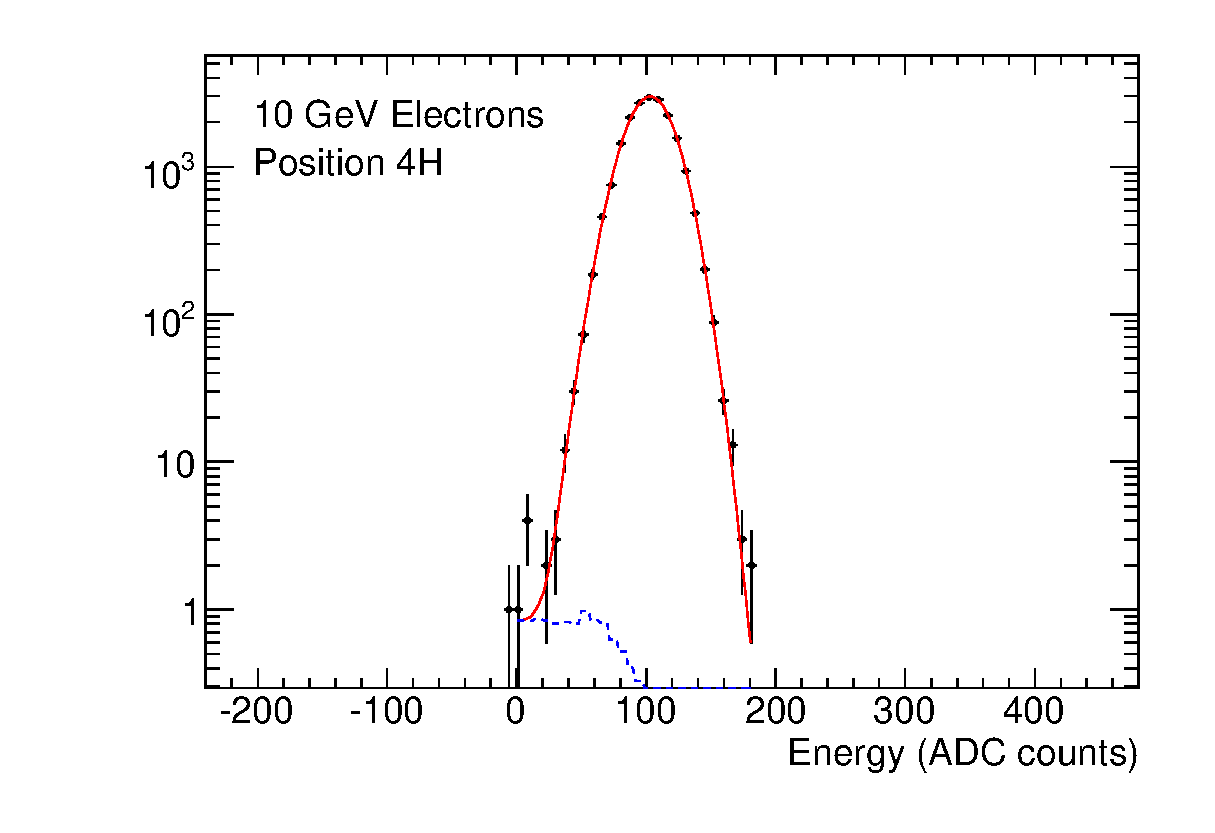
\includegraphics[width=0.45\linewidth,angle=0]{FCalTB_plots/Response_individual_data/Electron_response_10GeV_4H_data.eps}}
\end{center}
\caption{Response of the FCal to electrons directed at position 4H.}
\label{TBplot_electron_response_4H_data}
\end{figure}

%%%%%%%%%%%%%%%%%%%%%%%%%%%%%%%%%%%%%%%%%%%%%%%%%%%%%%%%%%%%%%%
%electrons at 4L, c8
\begin{table}[p]
\begin{center}
\begin{tabular}{|l|l|l|l|}
\hline
Beam Energy (GeV) & Fitted Mean (ADC)& Fitted Width (ADC)& Noise (ADC) \\
\hline
193.1 GeV  &  2300.6 $\pm$     0.5 &    94.4 $\pm$     0.3 &    15.1 $\pm$     0.1 \\
147.8 GeV  &  1763.4 $\pm$     0.8 &    75.9 $\pm$     0.5 &    17.2 $\pm$     0.1 \\
100 GeV  &  1186.4 $\pm$     0.3 &    56.8 $\pm$     0.2 &    17.5 $\pm$     0.1 \\
80 GeV  &   946.9 $\pm$     0.3 &    47.9 $\pm$     0.2 &    17.4 $\pm$     0.1 \\
60 GeV  &   708.1 $\pm$     0.9 &    36.6 $\pm$     0.7 &    13.9 $\pm$     0.2 \\
40 GeV  &   472.4 $\pm$     0.2 &    29.9 $\pm$     0.1 &    14.6 $\pm$     0.1 \\
20 GeV  &   229.3 $\pm$     0.1 &    21.7 $\pm$     0.1 &    14.53 $\pm$     0.04 \\
10 GeV  &   110.9 $\pm$     0.1 &    17.7 $\pm$     0.1 &    14.5 $\pm$     0.1 \\
\hline
\end{tabular}
\end{center}
\caption{Results for the FCal response to electrons, directed at position 4L. Quoted errors are statistical only.}
\label{TBres_table_elec_4L}
\end{table}
%%%%%%%%%%%%%%%%%%%%%%%%%%%%%%%%%%%%%%%%%%%%%%%%%%%%%%%%%%%%%%%

%%%%%%%%%%%%%%%%%%%%%%%%%%%%%%%%%%%%%%%%%%%%%%%%%%%%%%%%%%%%%%%
\begin{table}[p]
\begin{center}
\begin{tabular}{|l|l|l|l|}
\hline
Beam Energy (GeV) & Fitted Mean (ADC)& Fitted Width (ADC)& Noise (ADC) \\
\hline
193.1 GeV  &  2263.9 $\pm$     0.7 &    90.9 $\pm$     0.5 &    15.7 $\pm$     0.1 \\
147.8 GeV  &  1718.3 $\pm$     0.8 &    72.1 $\pm$     0.5 &    15.6 $\pm$     0.1 \\
100 GeV  &  1150.8 $\pm$     0.3 &    55.1 $\pm$     0.2 &    17.1 $\pm$     0.1 \\
80 GeV  &   912.1 $\pm$     0.3 &    48.8 $\pm$     0.2 &    17.1 $\pm$     0.1 \\
60 GeV  &   680.1 $\pm$     0.4 &    40.5 $\pm$     0.2 &    15.9 $\pm$     0.1 \\
40 GeV  &   448.1 $\pm$     0.2 &    30.9 $\pm$     0.1 &    15.2 $\pm$     0.1 \\
20 GeV  &   215.8 $\pm$     0.1 &    23.1 $\pm$     0.1 &    14.85 $\pm$     0.05 \\
10 GeV  &   102.7 $\pm$     0.1 &    18.5 $\pm$     0.1 &    14.3 $\pm$     0.1 \\
%5 GeV  &    45.9 $\pm$     0.2 &    16.6 $\pm$     0.1 &    14.5 $\pm$     0.1 \\
\hline
\end{tabular}
\end{center}
\caption{Results for the FCal response to electrons, directed at position 4H. Quoted errors are statistical only.}
\label{TBres_table_elec_4H}
\end{table}
%%%%%%%%%%%%%%%%%%%%%%%%%%%%%%%%%%%%%%%%%%%%%%%%%%%%%%%%%%%%%%%


A double Gaussian is fit to the electron peak in the response distribution. While the beam envelope cuts improve the purity of the electron sample, some of these events still contain showers initiated by hadrons. A feature of hadronic showers is that not all of the shower's energy is visible to the calorimeter. For example, when a nucleus breaks up as a result of an interaction with a showering hadron, an amount of nuclear binding energy is lost from the products of the reaction. Alternatively, hadronic interactions may lead to the production of a neutrino, which will carry energy out of the detector. Hadronic showers also produce kaons and charged pions, which may then decay weakly to produce muons. Muons produced in this way will deposit a minimal amount of energy in the active regions before leaving the calorimeter. Energy lost in processes such as these cannot be measured by the calorimeter, resulting in a response lower than that seen for an EM particle with the same energy \footnote{Compensating calorimeters (such as ZEUS\cite{zeus}) are designed to correct for this effect, such that the response to hadrons will be equal to that for electrons of the same energy.}.


% For this reason, the energy reconstructed at the EM scale is some fraction of the energy of the incident hadron, typically around 60-80\% for the beam energies considered in this analysis.
%
%
%
%Hadronic showers deposit less visible energy in the calorimeter than electromagnetic showers. As the FCal is a non-compensating calorimeter, it therefore has a lower response to hadrons than it would to electrons of the same energy.


 

The response plots in Figures~\ref{TBplot_electron_response_4L_data} and \ref{TBplot_electron_response_4H_data} thus contain some events at lower energy due to the hadron contamination in addition to the higher energy peak corresponding to the electron response. The high tail of the hadron distribution overlaps with the low tail of the electron peak, and so this effect is accounted for when analysing the data. This is accomplished by including data taken from hadron runs into the fit for the electron response. The total function fitted to the distributions shown in Figure~\ref{TBplot_electron_response_4L_data} is given by
\begin{equation}
G(E) = F(E) + w \, H_\pi(E),
\end{equation}
where $F(E)$ is the double Gaussian function described in equation~\ref{eqn_dbl_Gaussian}. The ``function'' $H_\pi(E)$ is derived from data taken during pion runs. Cylindrical clusters with radius 8 cm are formed for each pion event, and used to fill a histogram with the same binning as is used for the electron response. The energy $E$ is then converted to a bin number, and the number of entries in this bin is taken as the value of $H_\pi(E)$. The parameter $w$ corresponds to a normalisation for the hadron data and is allowed to freely vary in the fitting. The parameters of the double Gaussian are also allowed to vary, but are subject to the constraints in equations~\ref{eqn_constraint_1} and \ref{eqn_constraint_2}.


The effects of the electronics noise are estimated by creating clusters from randomly triggered events. For each physics event, a randomly triggered event taken from the same run is chosen at random and reconstructed. The beam impact point from the physics event is used in the randomly triggered event, and a cylindrical cluster is formed around this point. As the cluster formed from the randomly triggered event uses the same impact point as is used in the physics event, the same calorimeter cells are clustered in each case.  A Gaussian fit is then performed on the cluster energies obtained from randomly triggered events, and the width of this is used as an estimate of the noise contribution to clusters formed from physics events. This width is used in the computation of the energy resolution, which is described below. 
%%%%%%%%%%%%%%%%%%%%%%%%%%%%%%%%%%%%%%%%%%%%%%%%%%%%%%%%%%%%%%%
%\begin{figure}[!htb]
%\begin{center}
%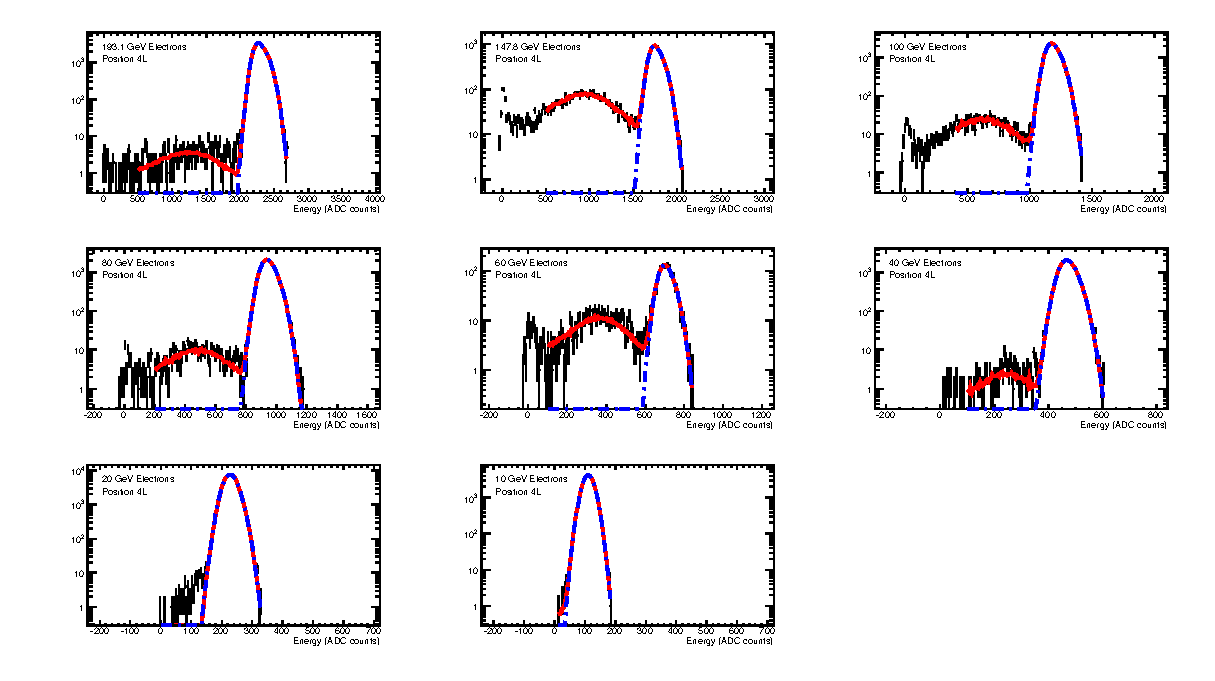
\includegraphics[width=1.0\linewidth,angle=0]{FCalTB_plots/electron_response_4L_data.eps}
%\end{center}
%\caption{Response of the FCal to electron beams directed at position 4L. The blue dashed curve double Gaussian fit to the electron peak, while the red curve shows the total fit to the electron peak plus the contaminant hadron contribution.}
%\label{TBplot_electron_response_4L_data}
%\end{figure}







The simulated response to electrons is shown in Figure~\ref{TB_electron_MC_response_4L} for position 4L and Figure~\ref{TBplot_electron_response_4H_MC} for position 4H, and these results are summarized in Tables \ref{TBres_table_elec_4LMC} and \ref{TBres_table_elec_4HMC}. All of the physics lists listed in section~\ref{TB_overview_g4} model electromagnetic showers in the same way, so no distinction between physics lists is made for the simulation results presented in this section. 

%noise noise noise.



%%%%%%%%%%%%%%%%%%%%%%%%%%%%%%%%%%%%%%%%%%%%%%%%%%%%%%%%%%%%%%%%
%\begin{figure}[!htb]
%\begin{center}
%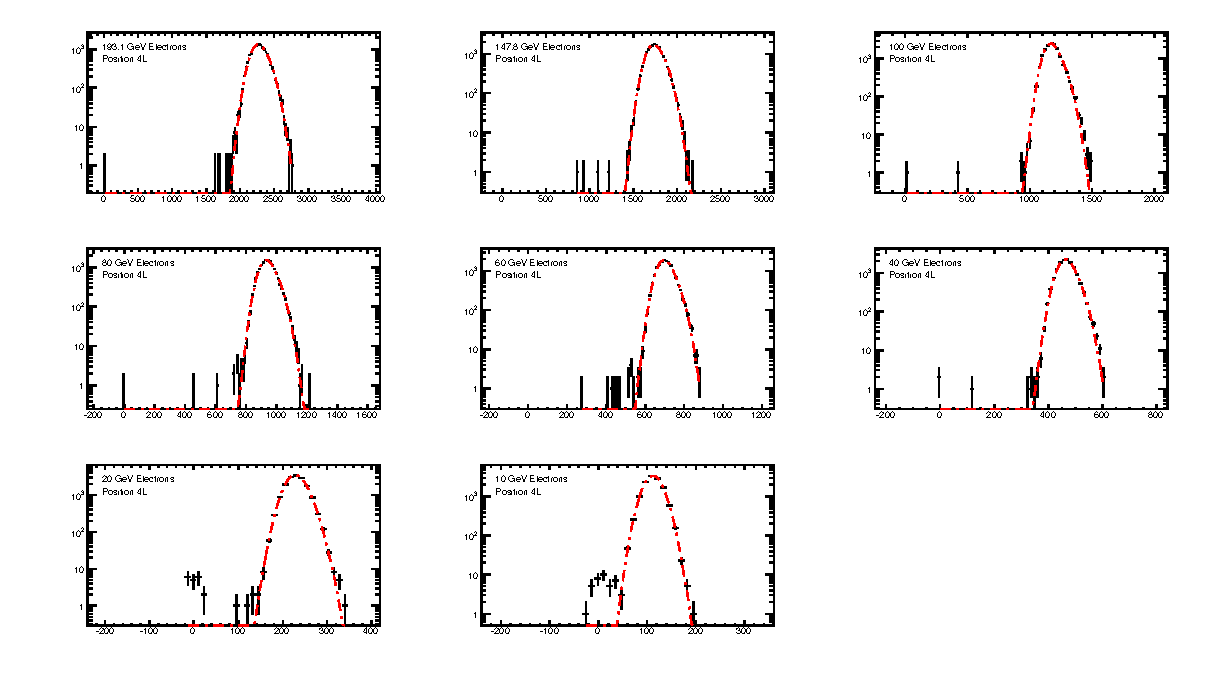
\includegraphics[width=1.0\linewidth,angle=0]{FCalTB_plots/electron_response_4L_MC.eps}
%\end{center}
%\caption{Monte Carlo results for electron beams directed at position 4L.}
%\label{TBplot_electron_response_4L_MC}
%\end{figure}
%%%%%%%%%%%%%%%%%%%%%%%%%%%%%%%%%%%%%%%%%%%%%%%%%%%%%%%%%%%%%%%%
%%%%%%%%%%%%%%%%%%%%%%%%%%%%%%%%%%%%%%%%%%%%%%%%%%%%%%%%%%%%%%%
\begin{figure}[p]
\begin{center}
\subfigure{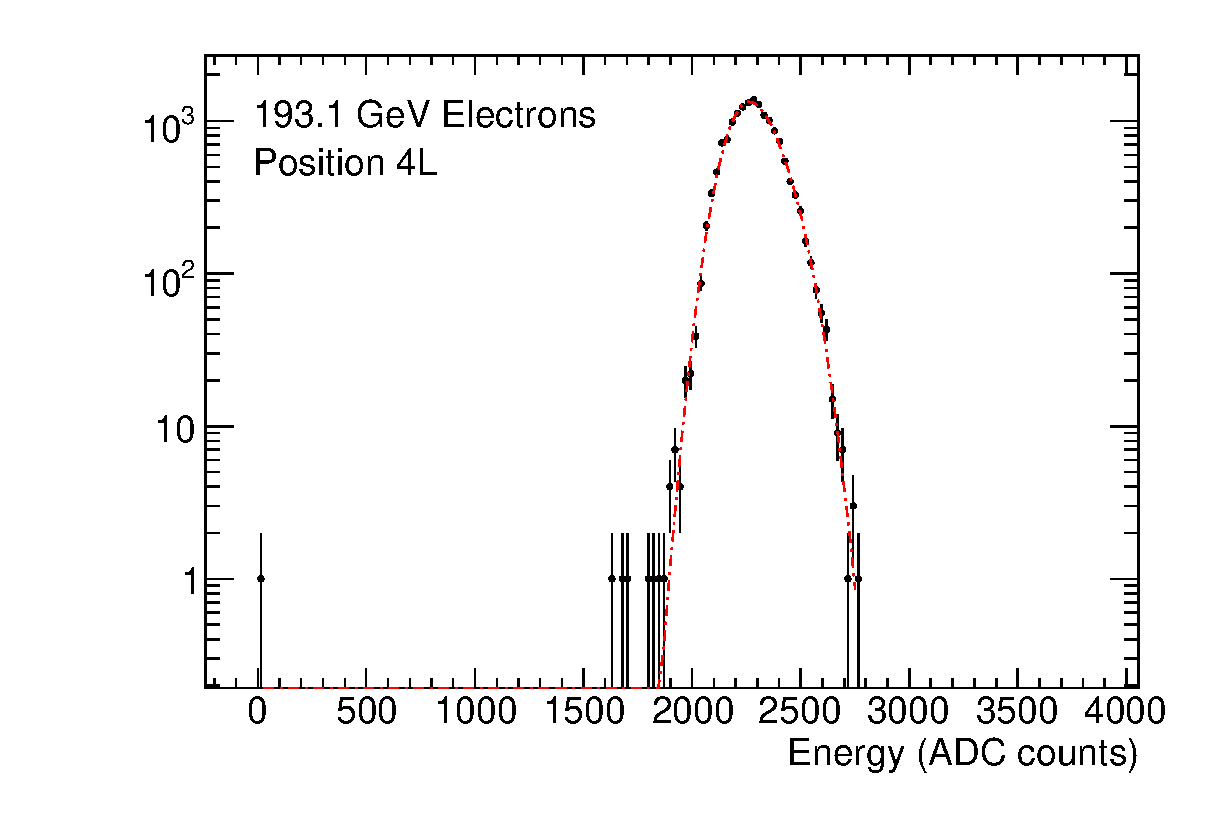
\includegraphics[width=0.45\linewidth,angle=0]{FCalTB_plots/Response_individual_MC/Electron_response_193GeV_4L_MC.eps}}
\subfigure{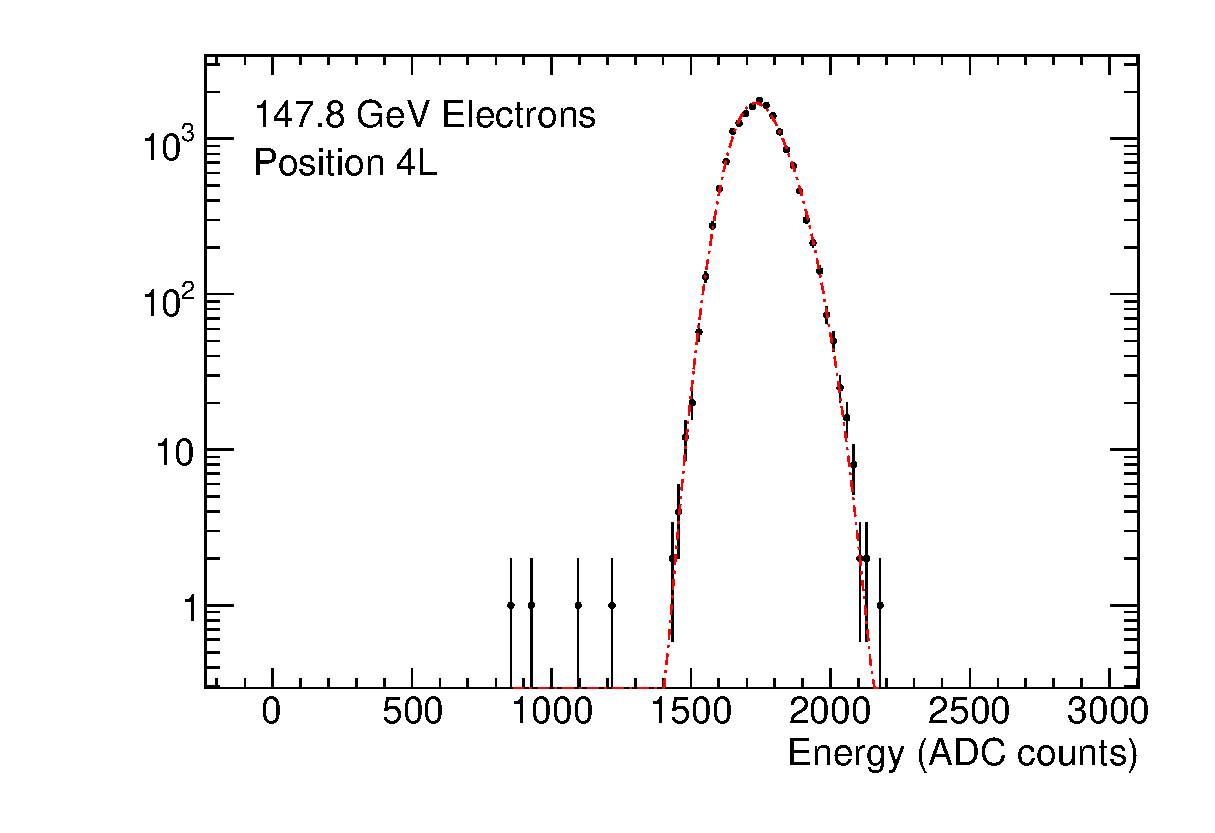
\includegraphics[width=0.45\linewidth,angle=0]{FCalTB_plots/Response_individual_MC/Electron_response_148GeV_4L_MC.eps}}\\
\subfigure{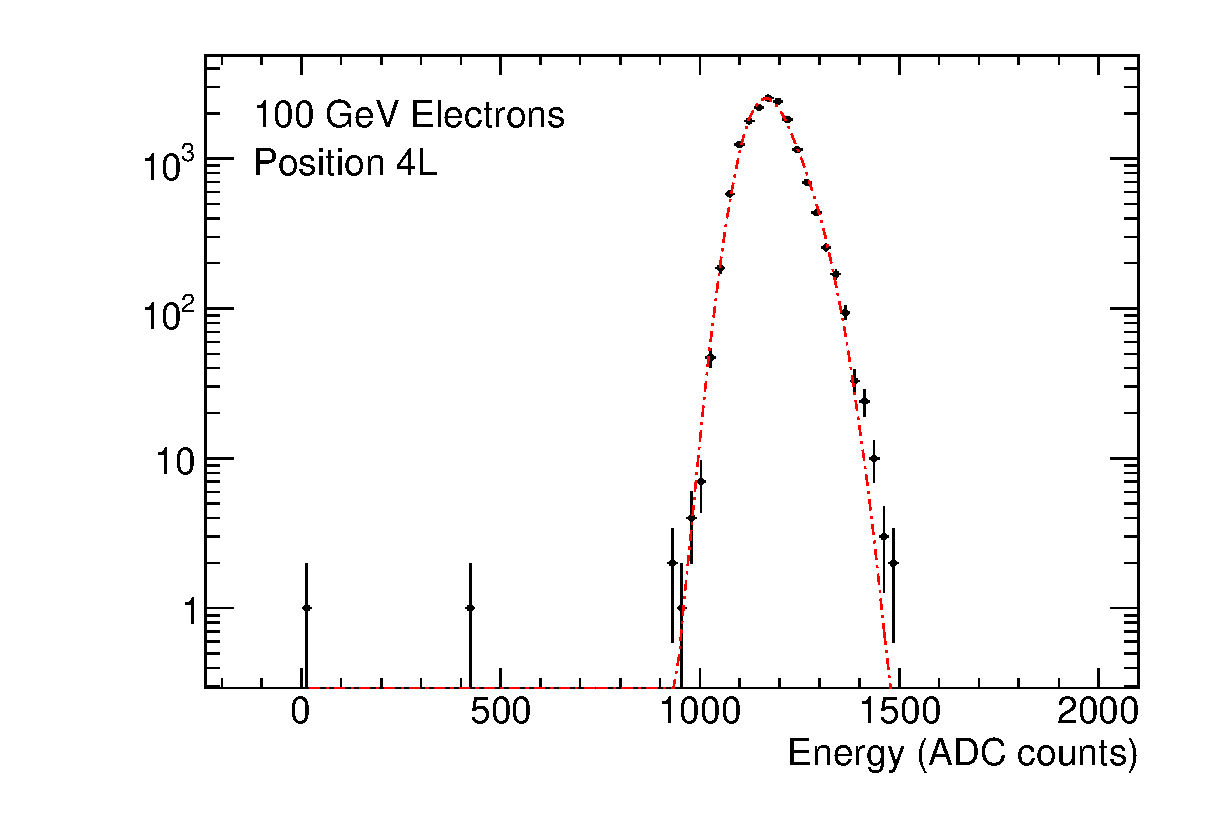
\includegraphics[width=0.45\linewidth,angle=0]{FCalTB_plots/Response_individual_MC/Electron_response_100GeV_4L_MC.eps}}
\subfigure{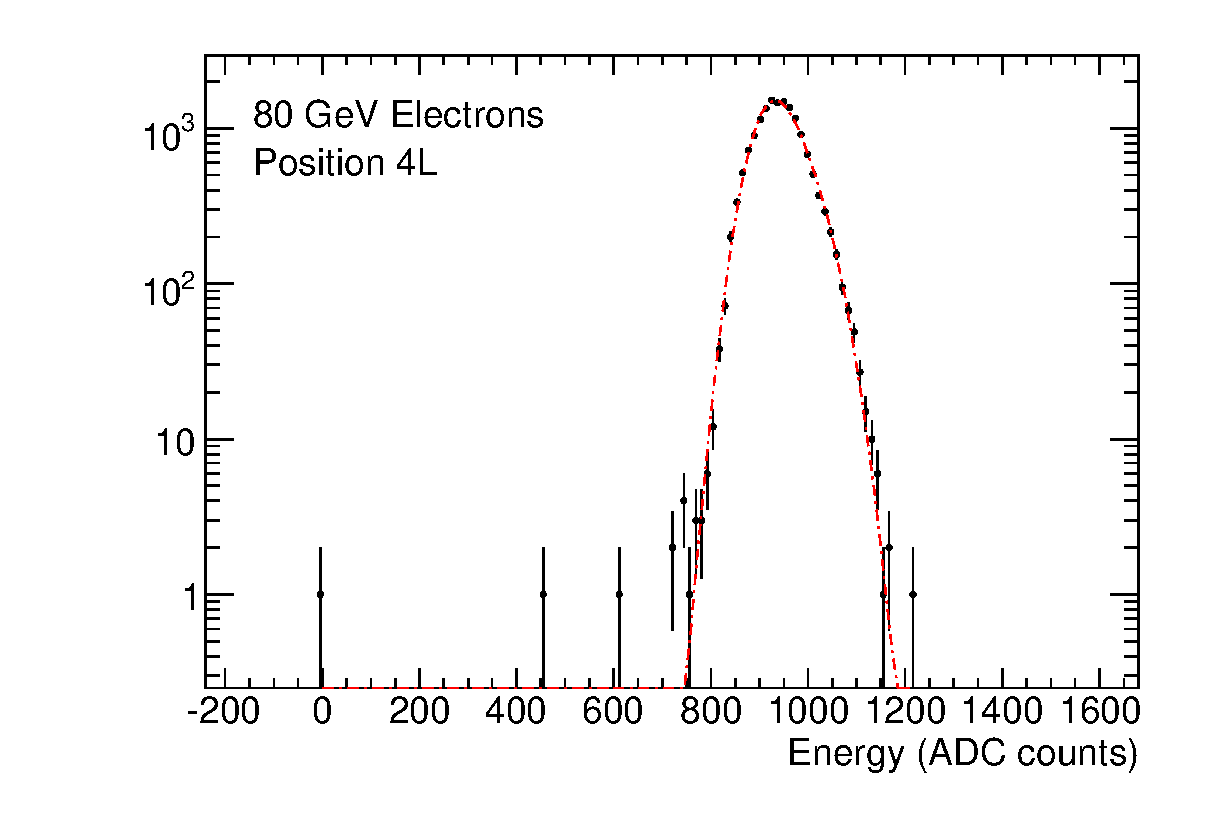
\includegraphics[width=0.45\linewidth,angle=0]{FCalTB_plots/Response_individual_MC/Electron_response_80GeV_4L_MC.eps}}\\
\subfigure{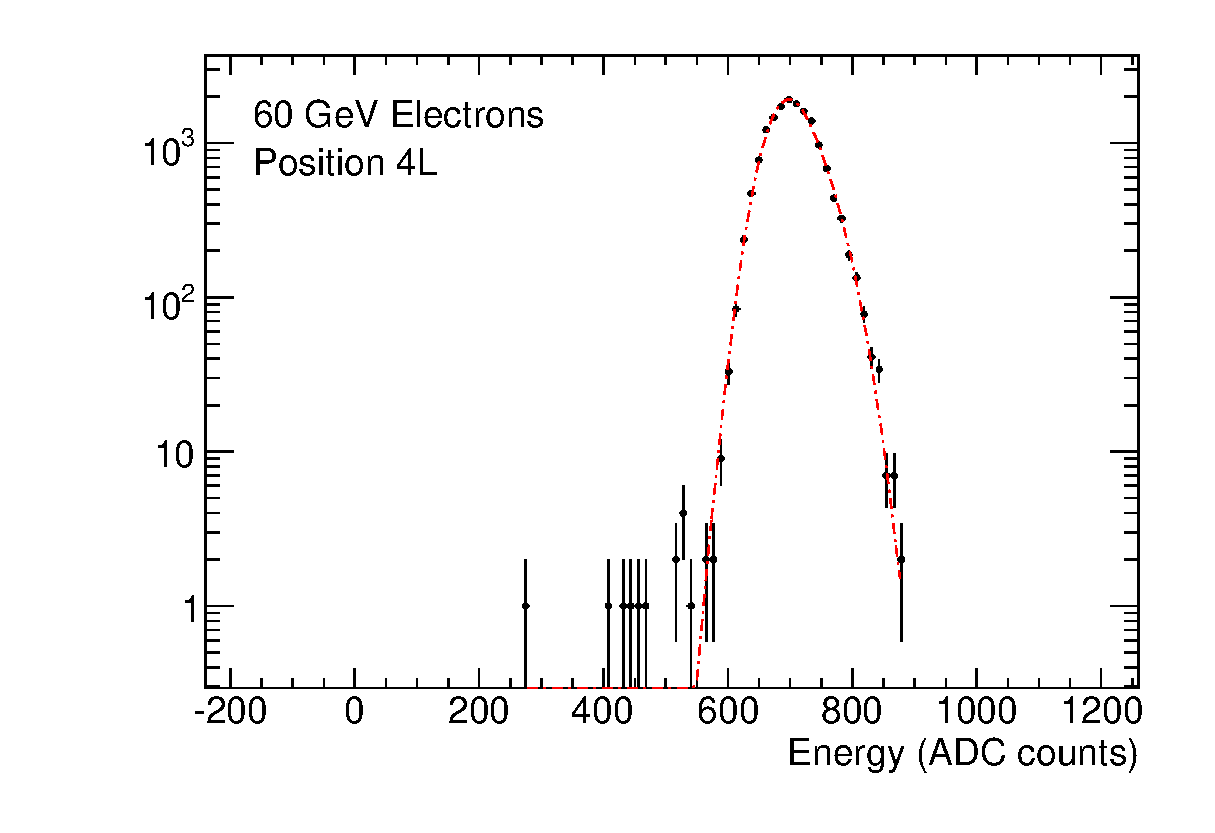
\includegraphics[width=0.45\linewidth,angle=0]{FCalTB_plots/Response_individual_MC/Electron_response_60GeV_4L_MC.eps}}
\subfigure{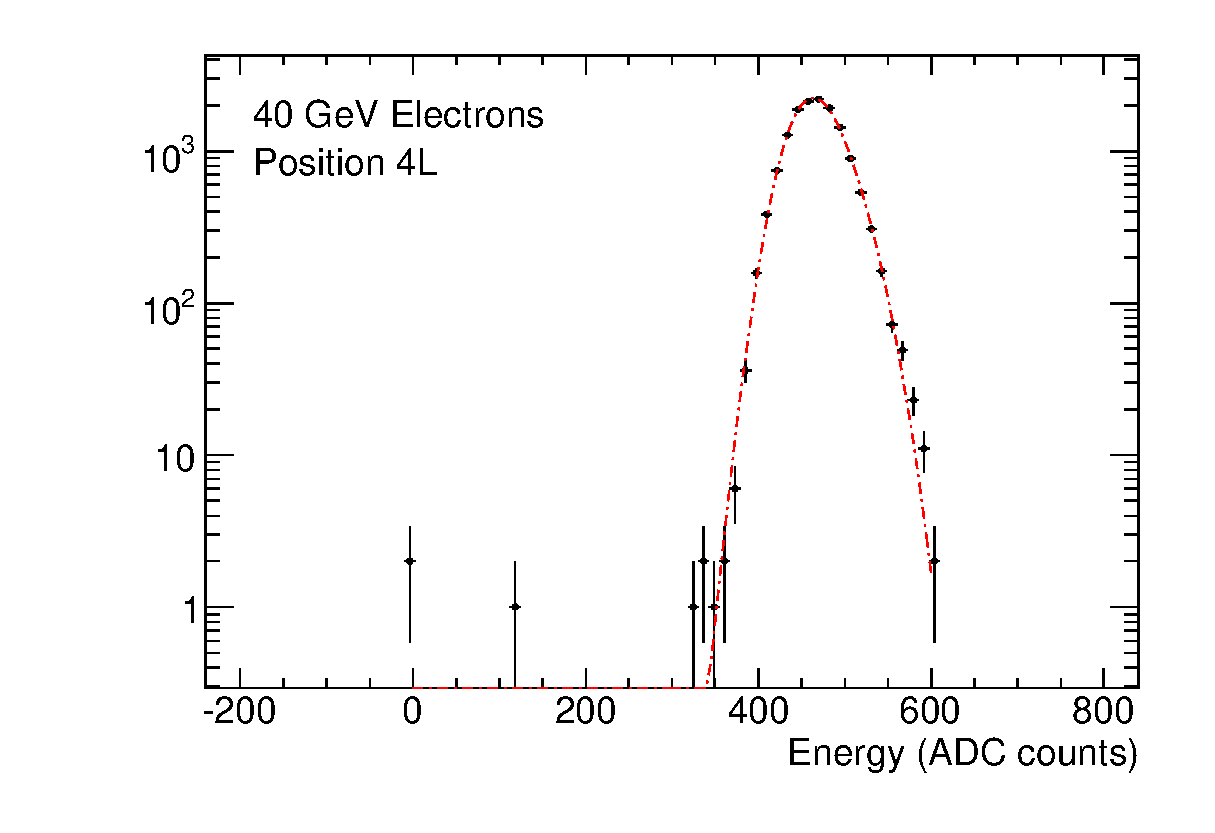
\includegraphics[width=0.45\linewidth,angle=0]{FCalTB_plots/Response_individual_MC/Electron_response_40GeV_4L_MC.eps}}\\
\subfigure{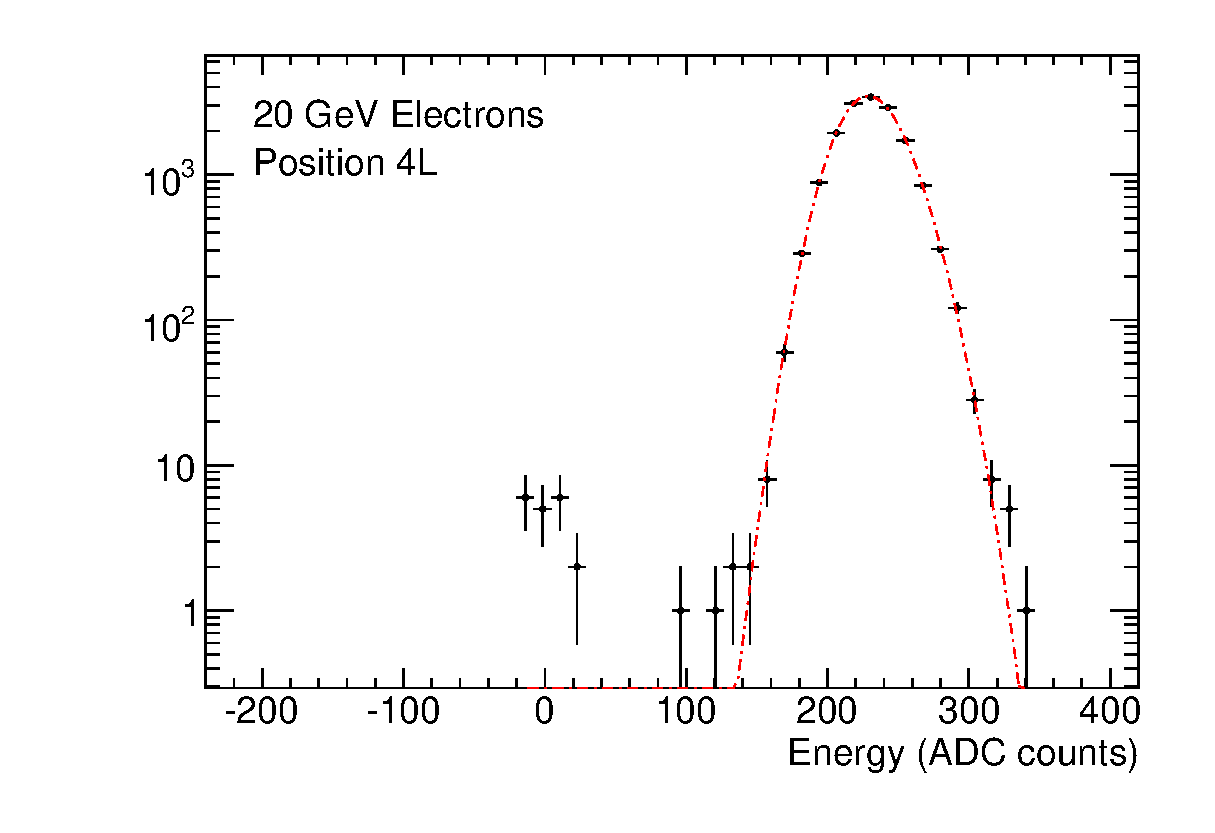
\includegraphics[width=0.45\linewidth,angle=0]{FCalTB_plots/Response_individual_MC/Electron_response_20GeV_4L_MC.eps}}
\subfigure{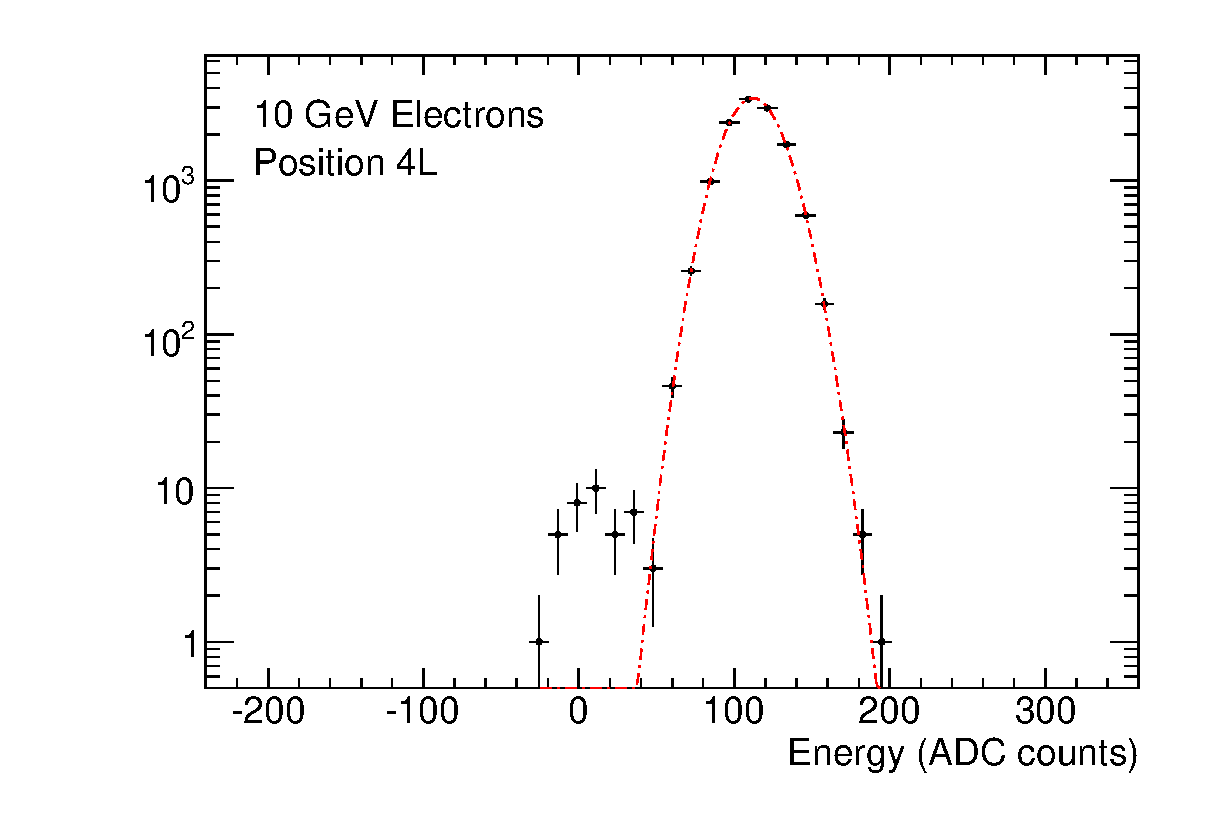
\includegraphics[width=0.45\linewidth,angle=0]{FCalTB_plots/Response_individual_MC/Electron_response_10GeV_4L_MC.eps}}\\
\end{center}
\caption{Monte Carlo results for electrons directed at position 4L.}
\label{TB_electron_MC_response_4L}
\end{figure}

%%%%%%%%%%%%%%%%%%%%%%%%%%%%%%%%%%%%%%%%%%%%%%%%%%%%%%%%%%%%%%%
%maybe some words go here
%%%%%%%%%%%%%%%%%%%%%%%%%%%%%%%%%%%%%%%%%%%%%%%%%%%%%%%%%%%%%%%

\begin{figure}[p]
\begin{center}
\subfigure{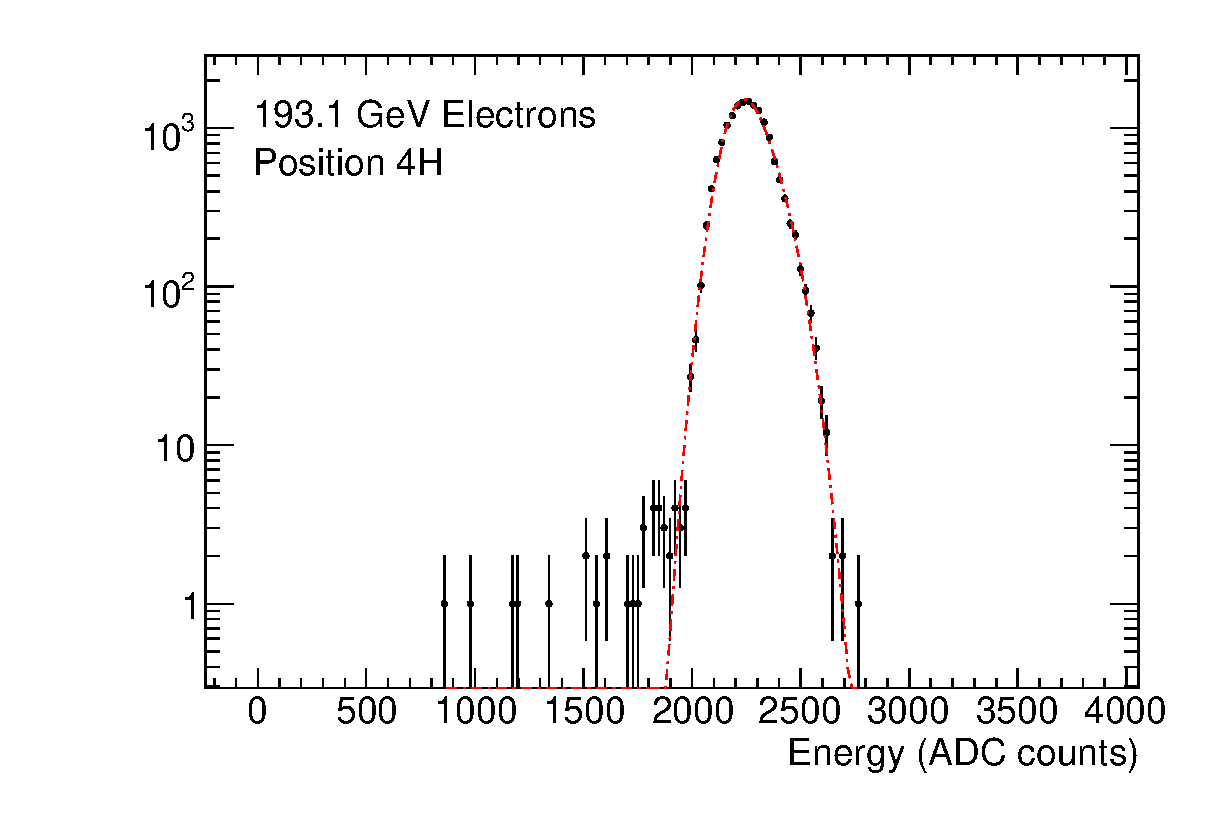
\includegraphics[width=0.45\linewidth,angle=0]{FCalTB_plots/Response_individual_MC/Electron_response_193GeV_4H_MC.eps}}
\subfigure{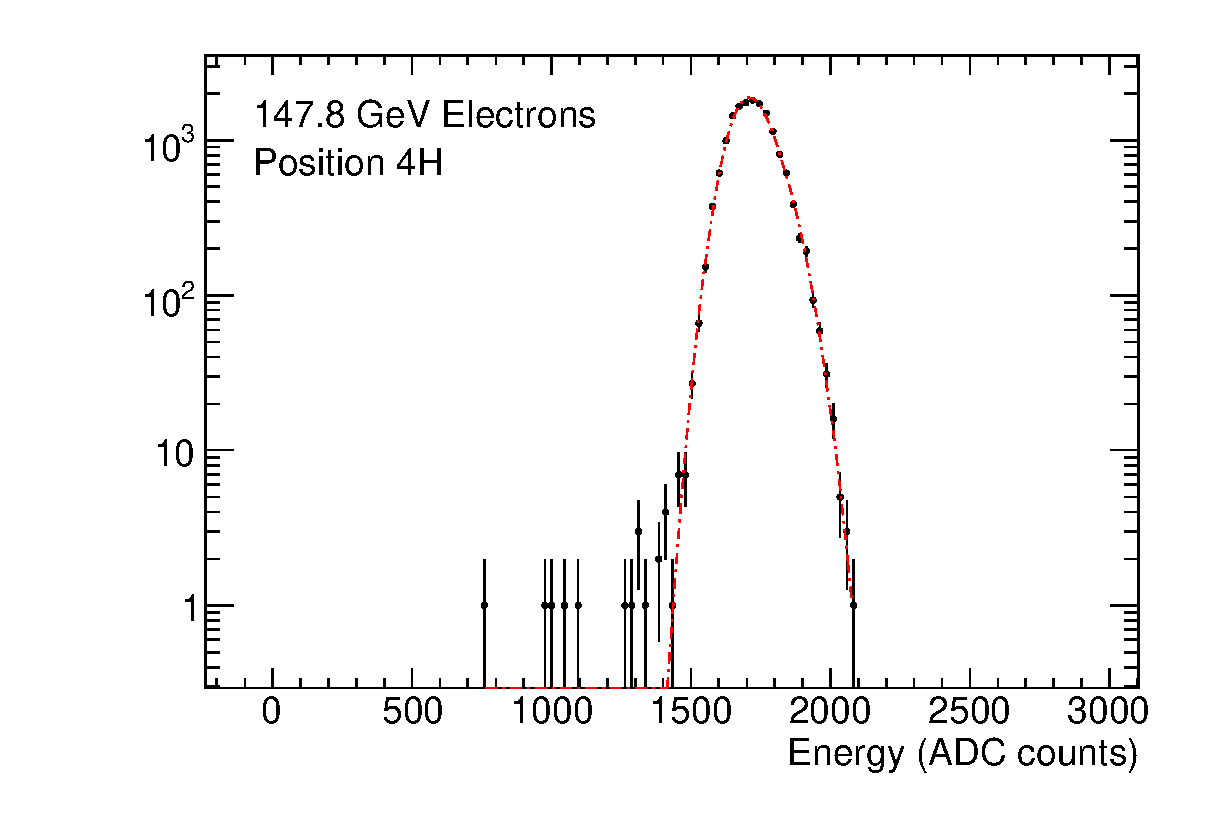
\includegraphics[width=0.45\linewidth,angle=0]{FCalTB_plots/Response_individual_MC/Electron_response_148GeV_4H_MC.eps}}\\
\subfigure{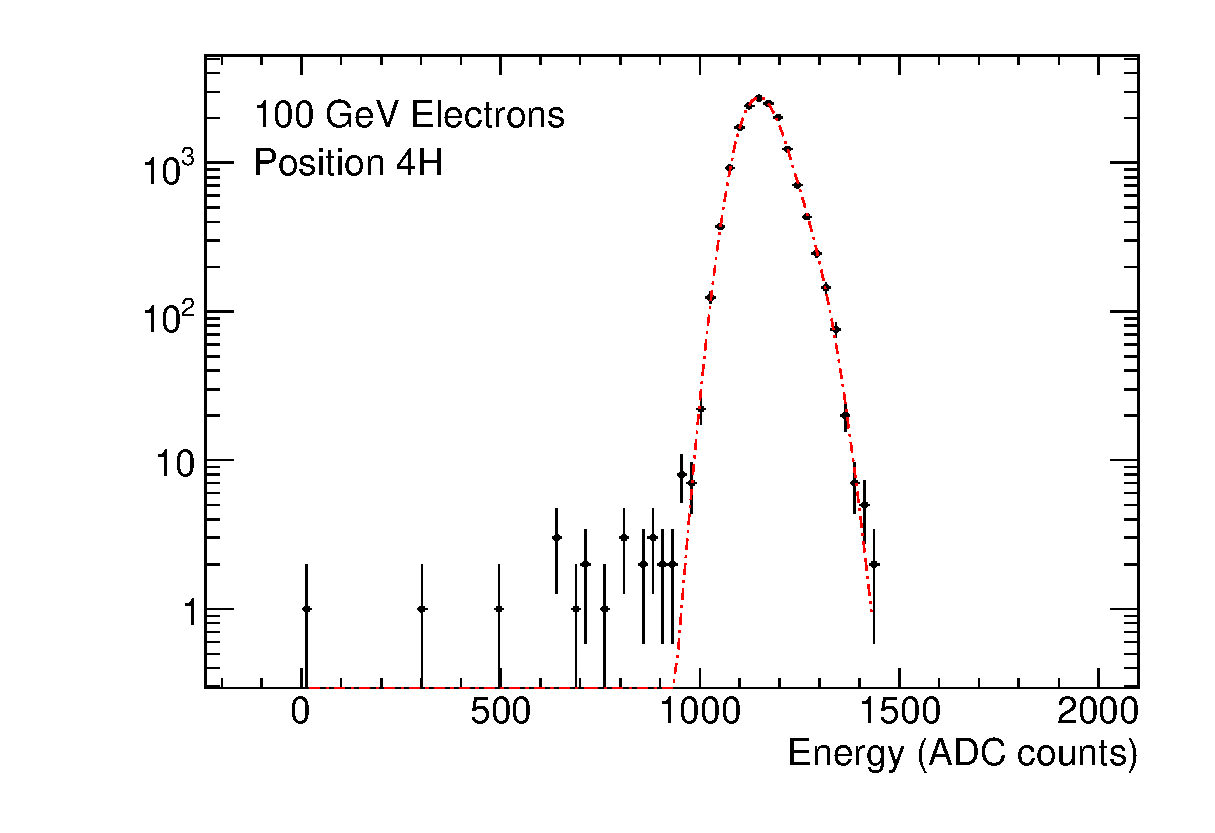
\includegraphics[width=0.45\linewidth,angle=0]{FCalTB_plots/Response_individual_MC/Electron_response_100GeV_4H_MC.eps}}
\subfigure{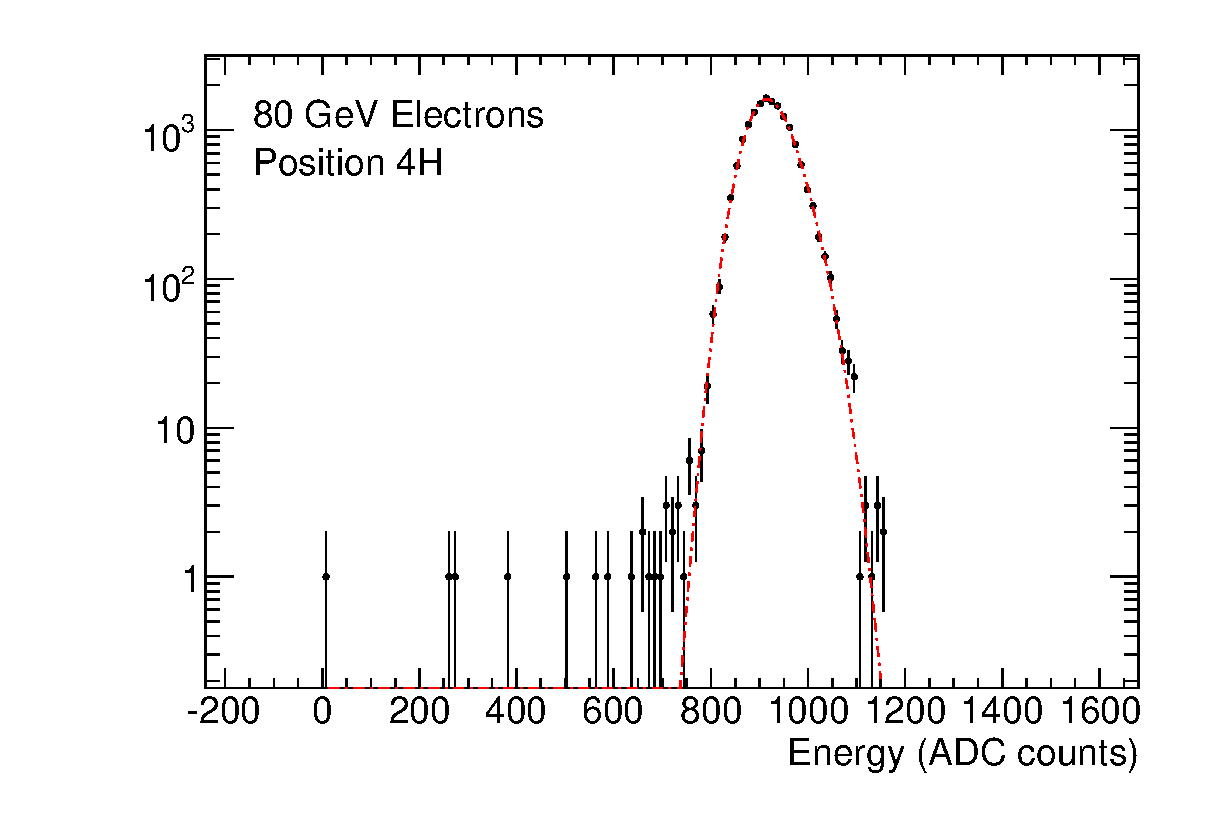
\includegraphics[width=0.45\linewidth,angle=0]{FCalTB_plots/Response_individual_MC/Electron_response_80GeV_4H_MC.eps}}\\
\subfigure{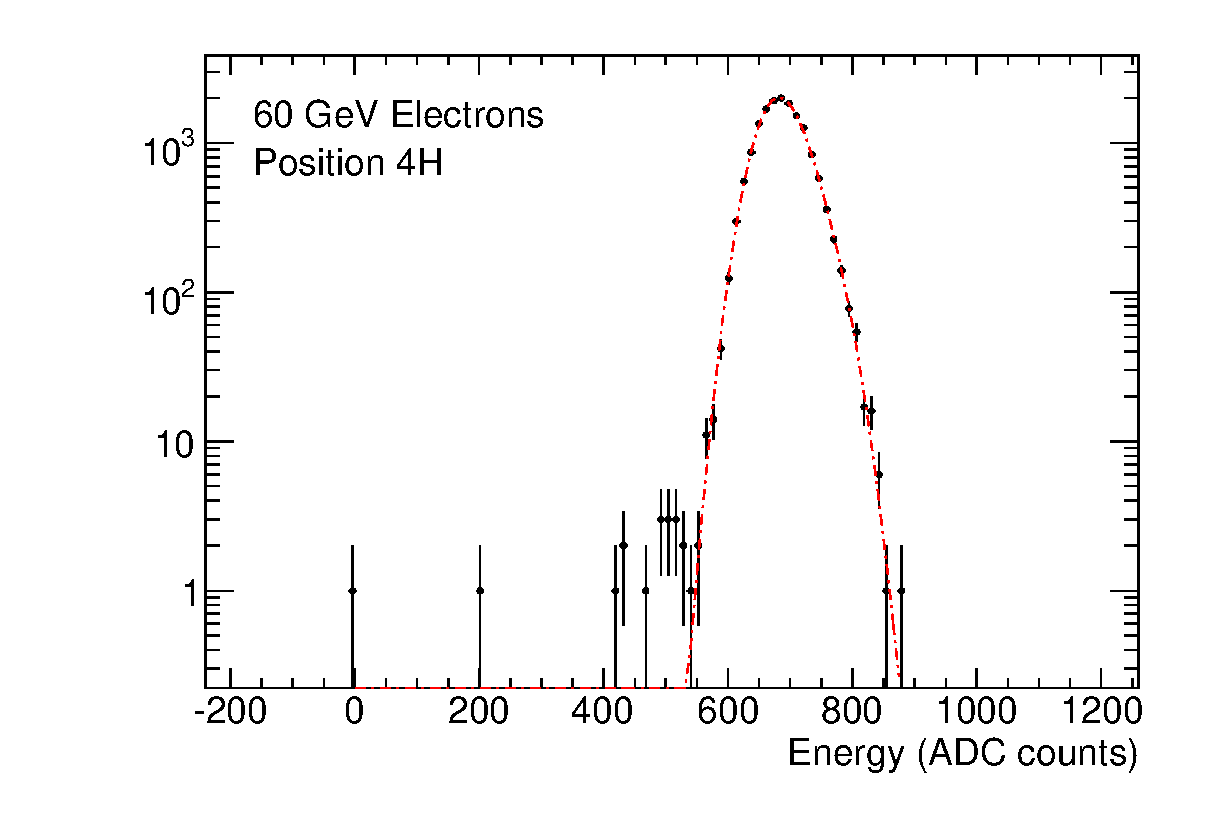
\includegraphics[width=0.45\linewidth,angle=0]{FCalTB_plots/Response_individual_MC/Electron_response_60GeV_4H_MC.eps}}
\subfigure{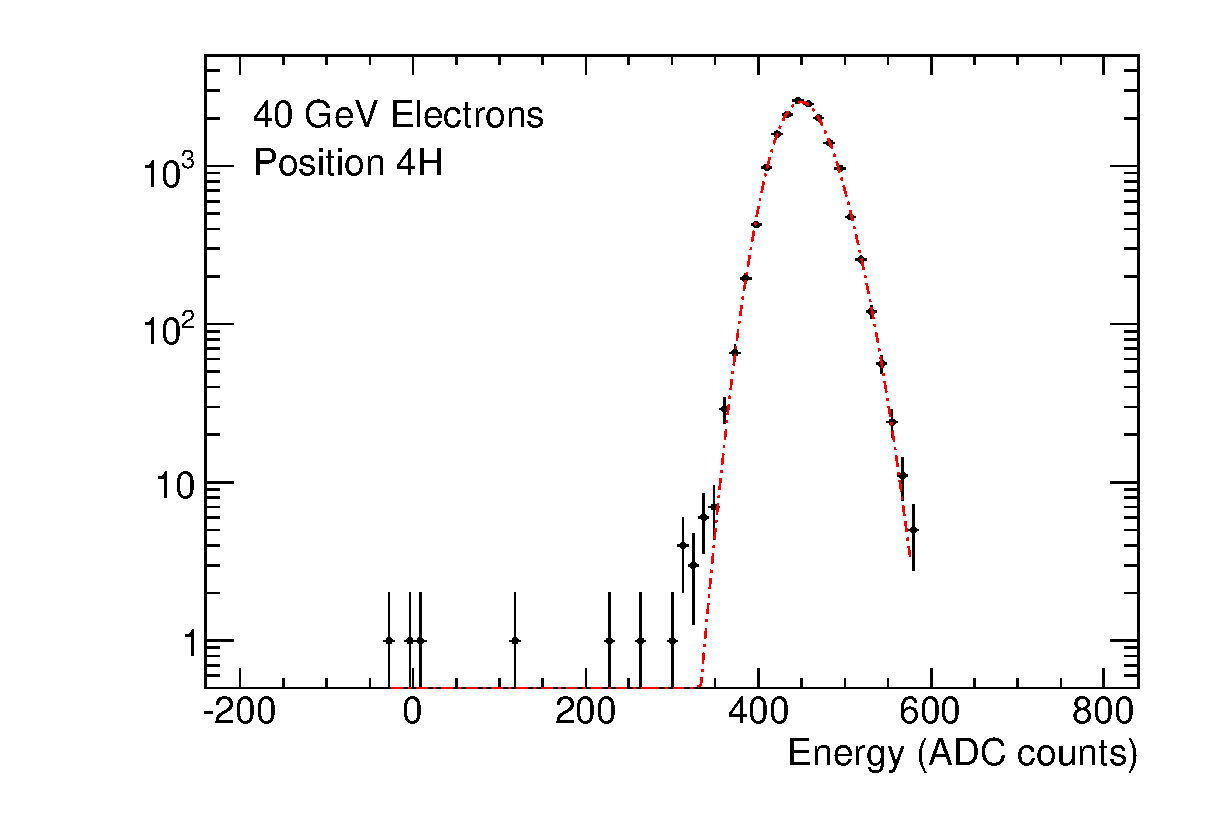
\includegraphics[width=0.45\linewidth,angle=0]{FCalTB_plots/Response_individual_MC/Electron_response_40GeV_4H_MC.eps}}\\
\subfigure{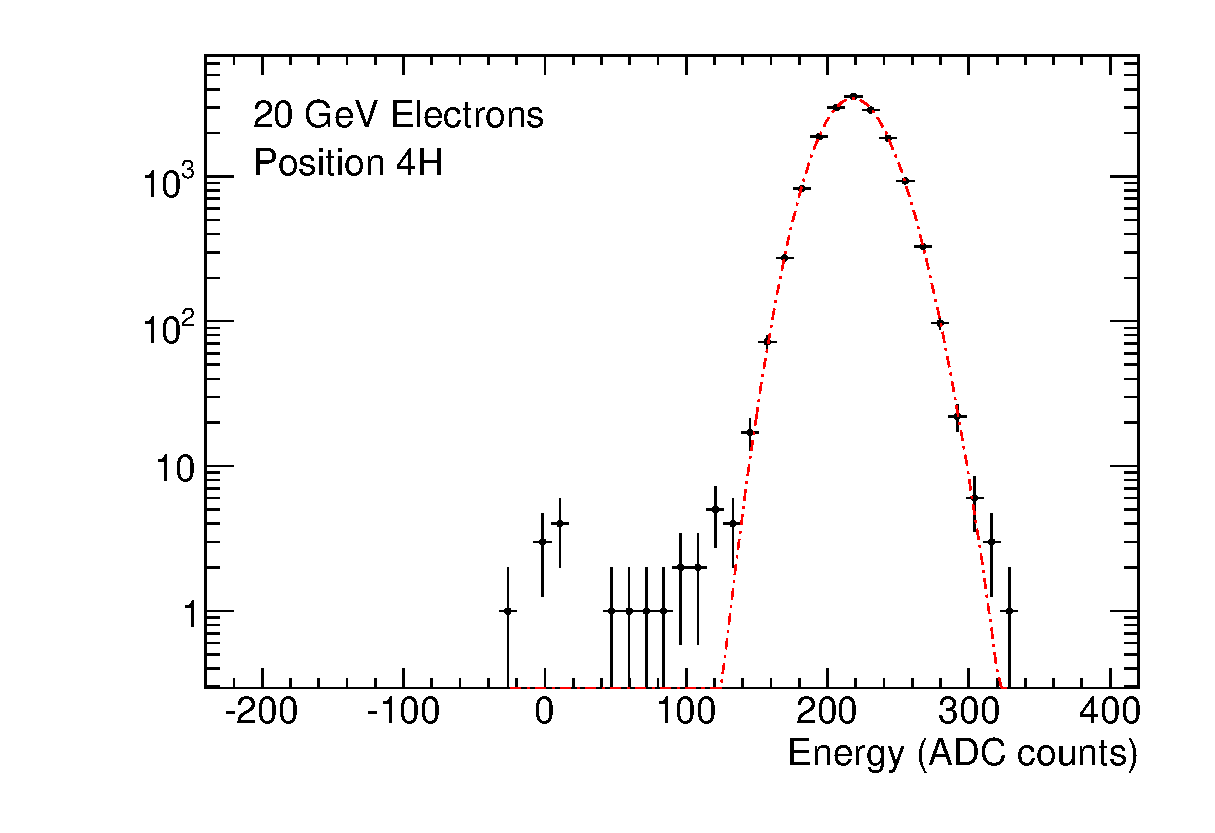
\includegraphics[width=0.45\linewidth,angle=0]{FCalTB_plots/Response_individual_MC/Electron_response_20GeV_4H_MC.eps}}
\subfigure{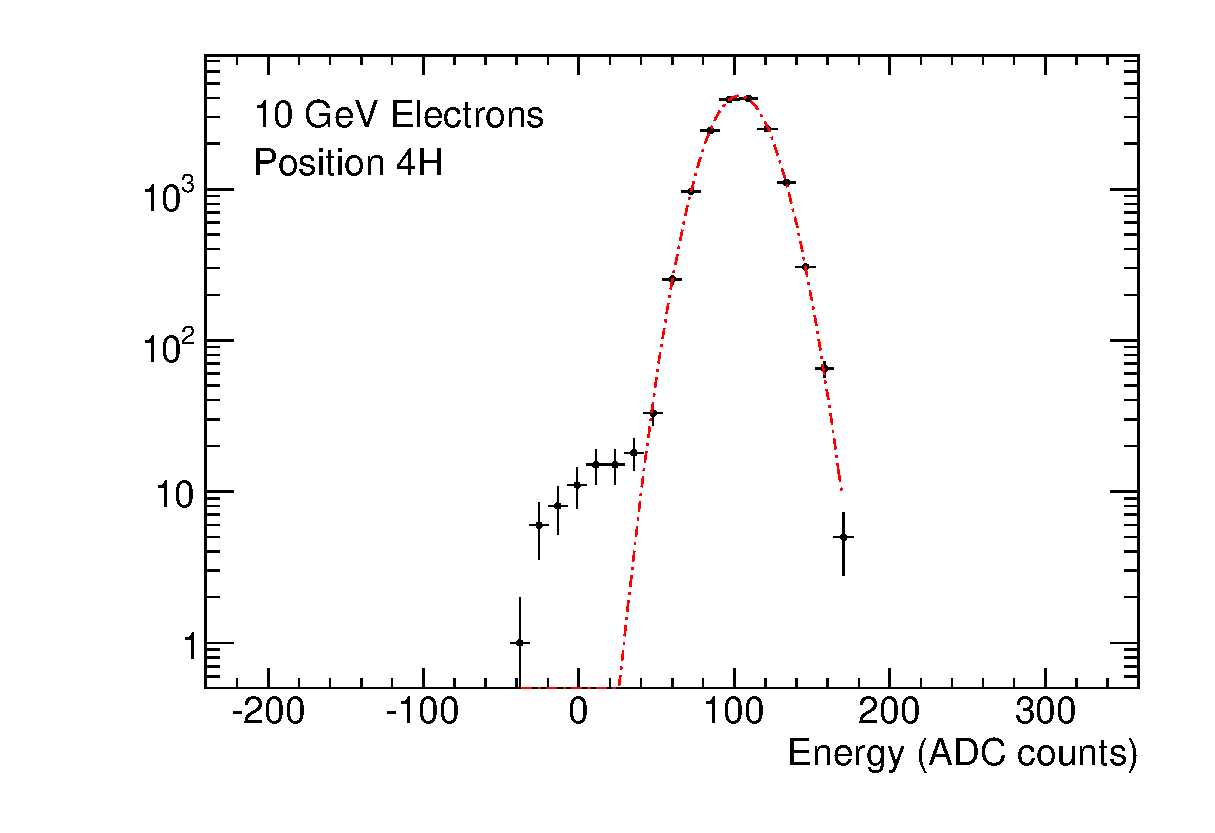
\includegraphics[width=0.45\linewidth,angle=0]{FCalTB_plots/Response_individual_MC/Electron_response_10GeV_4H_MC.eps}}\\
\end{center}
\caption{Monte Carlo results for electrons directed at position 4H.}
\label{TBplot_electron_response_4H_MC}
\end{figure}
%%%%%%%%%%%%%%%%%%%%%%%%%%%%%%%%%%%%%%%%%%%%%%%%%%%%%%%%%%%%%%%


%%%%%%%%%%%%%%%%%%%%%%%%%%%%%%%%%%%%%%%%%%%%%%%%%%%%%%%%%%%%%%%
\begin{table}[p]
\begin{center}
\begin{tabular}{|l|l|l|l|}
\hline
Beam Energy (GeV) & Fitted Mean (ADC)& Fitted Width (ADC)& Noise (ADC) \\
\hline
193.1 GeV  &  2285.2 $\pm$     0.9 &   114.3 $\pm$     0.7 &    14.2 $\pm$     0.1 \\
147.8 GeV  &  1747.4 $\pm$     0.7 &    91.3 $\pm$     0.5 &    17.0 $\pm$     0.1 \\
100 GeV  &  1180.2 $\pm$     0.5 &    62.5 $\pm$     0.3 &    17.4 $\pm$     0.1 \\
80 GeV  &   942.8 $\pm$     0.4 &    51.7 $\pm$     0.3 &    14.1 $\pm$     0.1 \\
60 GeV  &   705.3 $\pm$     0.3 &    40.9 $\pm$     0.2 &    14.2 $\pm$     0.1 \\
40 GeV  &   467.9 $\pm$     0.3 &    31.6 $\pm$     0.2 &    14.5 $\pm$     0.1 \\
20 GeV  &   230.5 $\pm$     0.2 &    22.2 $\pm$     0.1 &    14.3 $\pm$     0.1 \\
10 GeV  &   112.5 $\pm$     0.2 &    18.0 $\pm$     0.1 &    14.3 $\pm$     0.1 \\
5 GeV  &    53.1 $\pm$     0.1 &    16.9 $\pm$     0.1 &    14.1 $\pm$     0.1 \\
\hline
\end{tabular}
\end{center}
\caption{Simulated response of the FCal to electron beams directed at position 4L. Quoted uncertainties are statistical only.}
\label{TBres_table_elec_4LMC}
\end{table}
%%%%%%%%%%%%%%%%%%%%%%%%%%%%%%%%%%%%%%%%%%%%%%%%%%%%%%%%%%%%%%%

%maybe some words go here




%%%%%%%%%%%%%%%%%%%%%%%%%%%%%%%%%%%%%%%%%%%%%%%%%%%%%%%%%%%%%%%%
%\begin{figure}[!htb]
%\begin{center}
%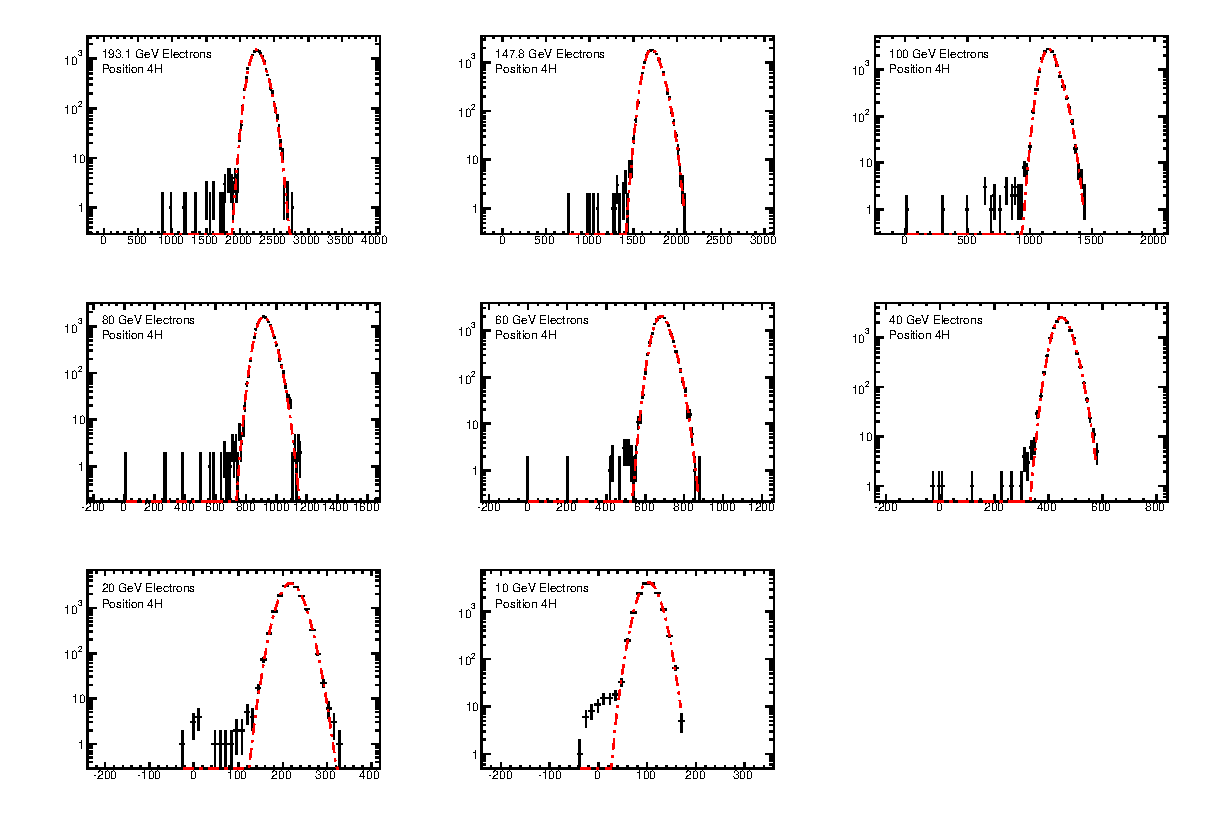
\includegraphics[width=1.0\linewidth,angle=0]{FCalTB_plots/electron_response_4H_MC.eps}
%\end{center}
%\caption{Monte Carlo results for electron beams directed at position 4H.}
%\label{TBplot_electron_response_4H_MC}
%\end{figure}
%%%%%%%%%%%%%%%%%%%%%%%%%%%%%%%%%%%%%%%%%%%%%%%%%%%%%%%%%%%%%%%%




%%%%%%%%%%%%%%%%%%%%%%%%%%%%%%%%%%%%%%%%%%%%%%%%%%%%%%%%%%%%%%%
\begin{table}[p]
\begin{center}
\begin{tabular}{|l|l|l|l|}
\hline
Beam Energy (GeV) & Fitted Mean (ADC)& Fitted Width (ADC)& Noise (ADC) \\
\hline
193.1 GeV  &  2259.7 $\pm$     0.8 &   103.2 $\pm$     0.6 &    15.9 $\pm$     0.1 \\
147.8 GeV  &  1723.5 $\pm$     0.7 &    82.8 $\pm$     0.5 &    15.6 $\pm$     0.1 \\
100 GeV  &  1159.5 $\pm$     0.4 &    58.4 $\pm$     0.3 &    17.0 $\pm$     0.1 \\
80 GeV  &   923.0 $\pm$     0.4 &    48.2 $\pm$     0.3 &    17.1 $\pm$     0.1 \\
60 GeV  &   687.7 $\pm$     0.3 &    39.3 $\pm$     0.2 &    16.1 $\pm$     0.1 \\
40 GeV  &   452.4 $\pm$     0.2 &    30.7 $\pm$     0.2 &    15.0 $\pm$     0.1 \\
20 GeV  &   218.8 $\pm$     0.2 &    22.3 $\pm$     0.1 &    14.6 $\pm$     0.1 \\
10 GeV  &   103.5 $\pm$     0.1 &    18.4 $\pm$     0.1 &    14.3 $\pm$     0.1 \\
\hline
\end{tabular}
\end{center}
\caption{Simulated response of the FCal to electron beams directed at position 4H. Quoted uncertainties are statistical only.}
\label{TBres_table_elec_4HMC}
\end{table}
%%%%%%%%%%%%%%%%%%%%%%%%%%%%%%%%%%%%%%%%%%%%%%%%%%%%%%%%%%%%%%%

The linearity of the FCal response to electrons is shown in Figures~\ref{TBplot_electron_linearity_4L} (for position 4L) and \ref{TBplot_electron_linearity_4H} (position 4H), depicting the mean reconstructed energy (in ADC counts) as a function of beam energy. The results of a linear fit have been overlaid, the results of which are given in Table \ref{table_electron_c8_linearity}. The $y$ intercept of the fit result was not fixed to zero when performing the fit, and was instead allowed to vary. The negative result for the intercept is attributed to energy losses in the upstream material, with the additional material at 4H resulting in an intercept larger in magnitude than that at 4L. As the simulation only modeled beamline components downstream of the B9 magnet, energy losses in materials upstream of this point would not be reflected in the simulation results. This is a possible explanation as to why the simulation results have a less negative intercept than those obtained from data. The effects of the additional material in front of position 4H appear to be well modelled by the simulation, as can be seen by comparing the values of the intercepts at position 4L and 4H. In data, the intercept at 4H is 8.3 ADC counts lower than that measured at position 4L, while in the simulation results there is a difference of 9.0 ADC counts. 


%The two dominant sources of systematic uncertainty on the linearity arise from the cluster radius and the beam polarity. 
One of the larger sources of systematic uncertainty on the linearity is due to effects related to the beam polarity. The electron beams used in this study were secondary or tertiary beams produced by directing proton beams from the SPS at a fixed target\cmt{lead}. At higher energies a secondary beam was used, the polarity of which ($e^+$ or $e^-$) was determined based on the needs of other experiments in the neighbouring H8 beamline. At lower energies a tertiary beam was used, the polarity of which could be chosen freely. %The magnets used in the beamline \red{ were not} systematically de-gaussed between runs at different beam polarities.
%Data taken at 4L with both e+ beams and e- beams is available at two energy points: 10~GeV and 20~GeV

Data was taken at position 4L using both $e^-$ and $e^+$ beams at energies of 10~GeV and 20~GeV. Electromagnetic showers induced by electrons should on average deposit the same energy as those initiated by positrons. The 10~GeV and 20~GeV results in Figure~\ref{TBplot_electron_response_4L_data} use data obtained from both $e^+$ and $e^-$ beams. When beams of opposite polarity were considered separately, the response to 10~GeV positrons was found to be on average 1.6\% higher than the response to electrons. At 20~GeV, the response to positrons is 1.0\% higher than the response to electrons. This variation in response is attributed to conditions in the magnet systems. The magnets were not systematically de-gaussed during data taking, and so it is possible that hysteresis effects may have led to some small fluctuations in the beam energy. These variations in the beam energy are considered as a source of systematic uncertainty.

% This variation in the response is atrrbuted to variations in the beam conditions. The beam magnets were not systematically de-gaussed, and so .
%
% This difference in response is attributed to variation in the beam conditions, and is considered as a source of systematic uncertainty. 


%e+ 1.6% higher than e- at 10~GeV, 4L
%e+ 1.0% higher than e- at 20~GeV





%%%%%%%%%%%%%%%%%%%%%%%%%%%%%%%%%%%%%%%%%%%%%%%%%%%%%%%%%%%%%%%%
%\begin{figure}[!htb]
%\begin{center}
%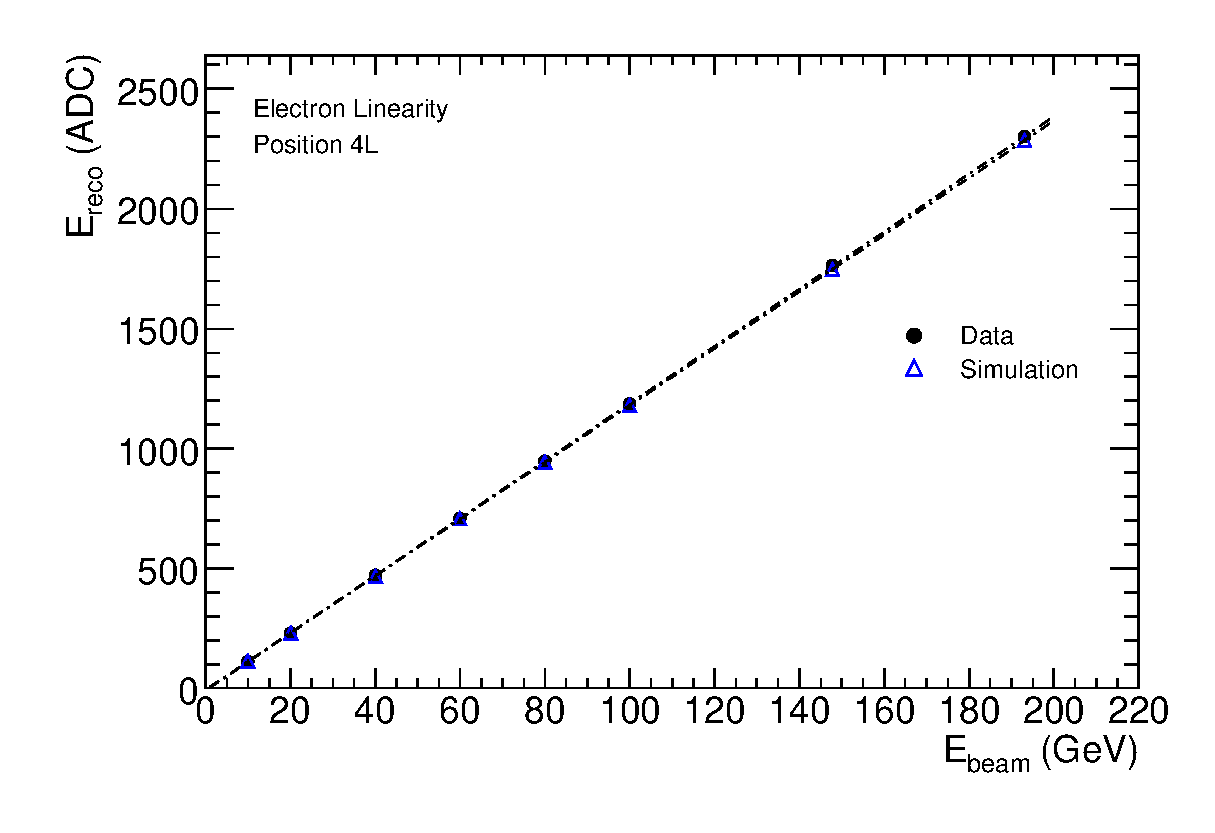
\includegraphics[width=0.95\linewidth,angle=0]{FCalTB_plots/electron_linearity_4L.eps}
%\end{center}
%\caption{Linearity of the response to electrons at position 4L. }
%\label{TBplot_electron_linearity_4L}
%\end{figure}
%%%%%%%%%%%%%%%%%%%%%%%%%%%%%%%%%%%%%%%%%%%%%%%%%%%%%%%%%%%%%%%%
%%%%%%%%%%%%%%%%%%%%%%%%%%%%%%%%%%%%%%%%%%%%%%%%%%%%%%%%%%%%%%%%
%\begin{figure}[!htb]
%\begin{center}
%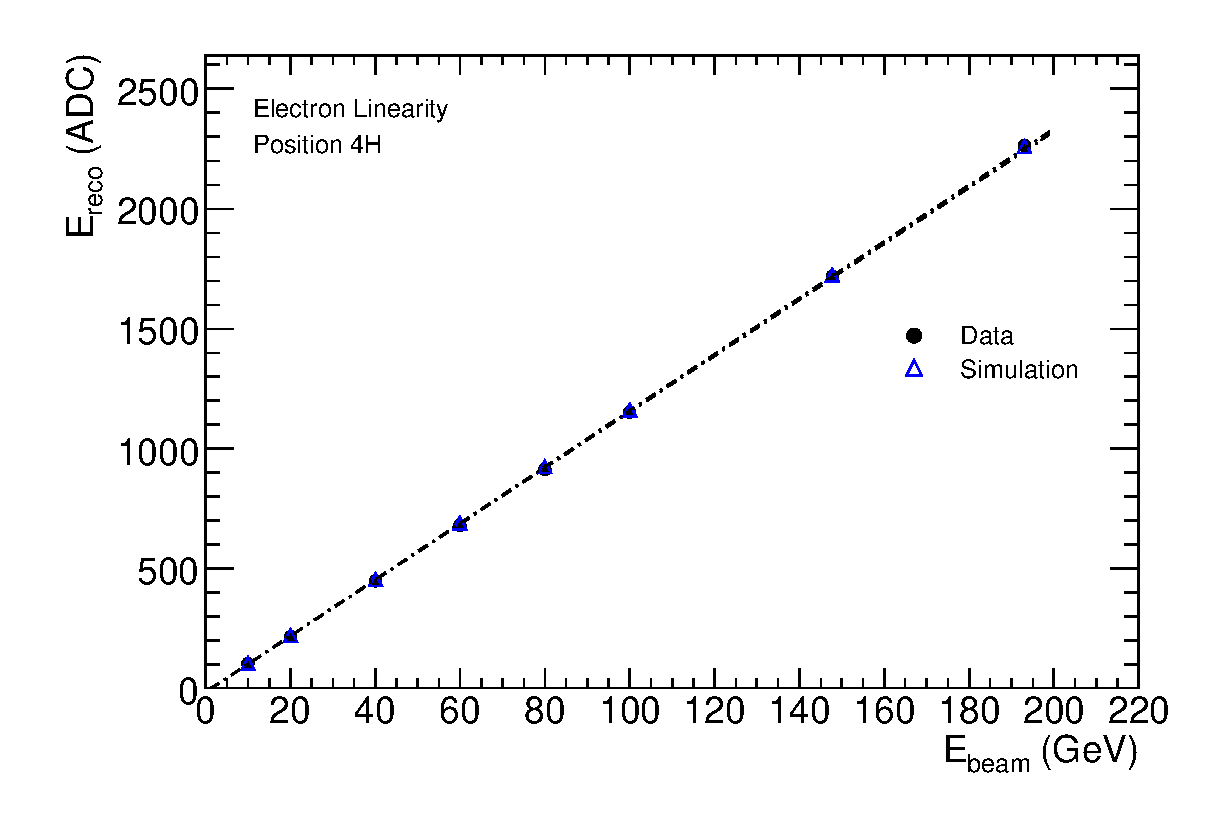
\includegraphics[width=0.95\linewidth,angle=0]{FCalTB_plots/electron_linearity_4H.eps}
%\end{center}
%\caption{Linearity of the response to electrons at position 4H. }
%\label{TBplot_electron_linearity_4H}
%\end{figure}
%%%%%%%%%%%%%%%%%%%%%%%%%%%%%%%%%%%%%%%%%%%%%%%%%%%%%%%%%%%%%%%%
%%%%%%%%%%%%%%%%%%%%%%%%%%%%%%%%%%%%%%%%%%%%%%%%%%%%%%%%%%%%%%%
\begin{figure}[!htb]
\begin{center}
\subfigure[]{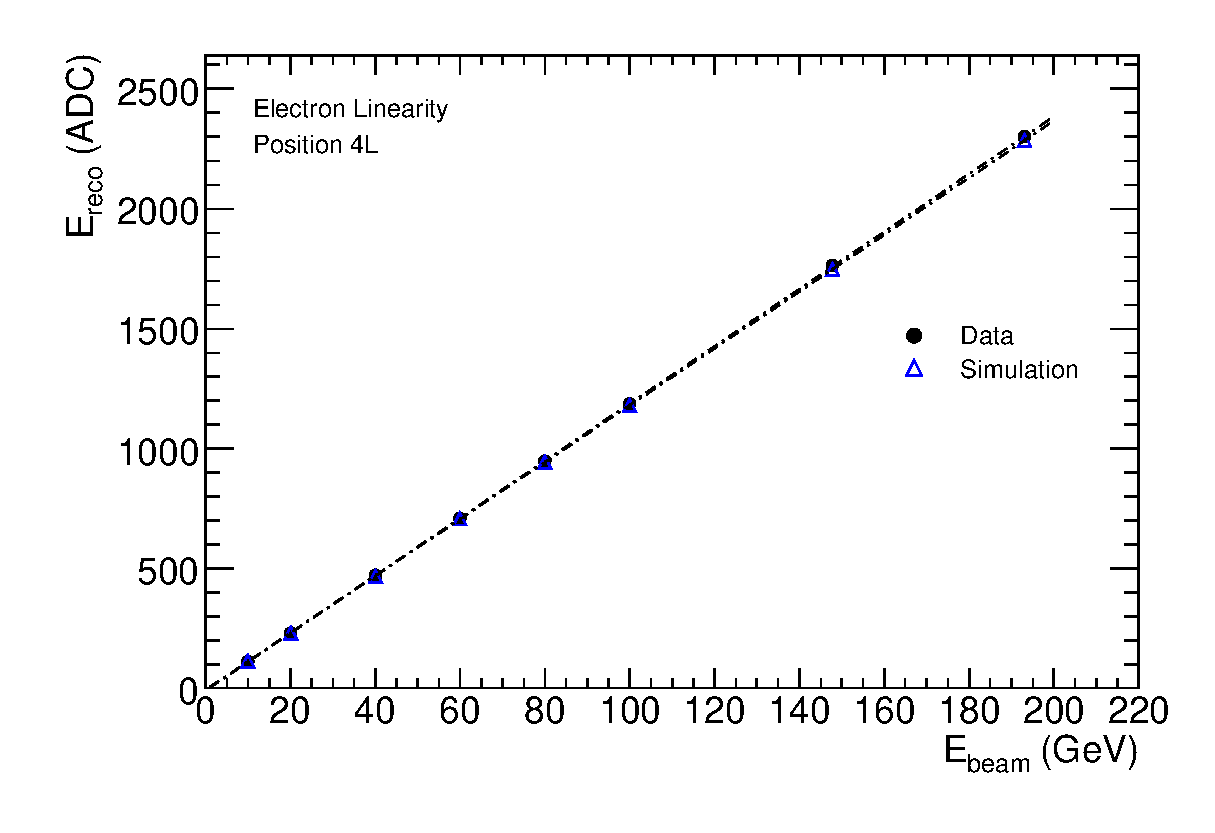
\includegraphics[width=0.45\linewidth,angle=0]{FCalTB_plots/electron_linearity_4L.eps}
\label{TBplot_electron_linearity_4L}}
\subfigure[]{
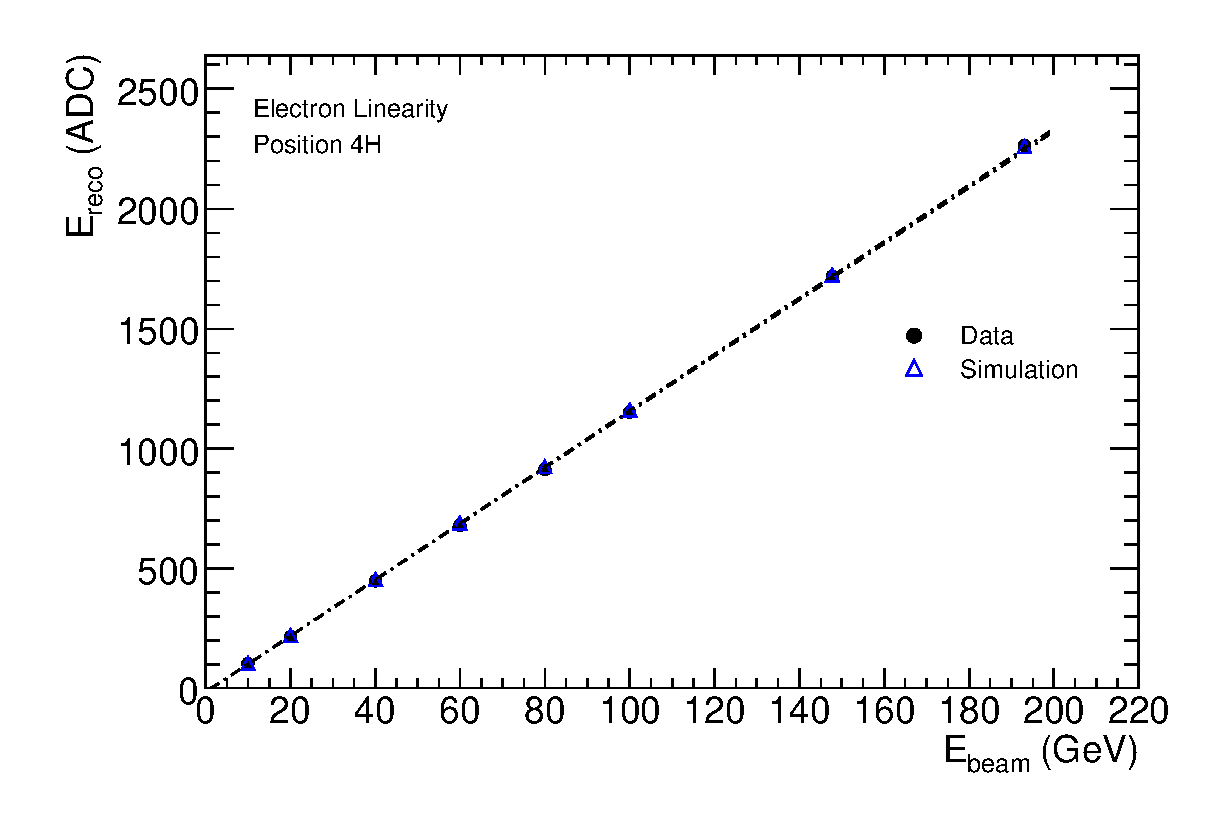
\includegraphics[width=0.45\linewidth,angle=0]{FCalTB_plots/electron_linearity_4H.eps}
\label{TBplot_electron_linearity_4H}
}
\caption{Linearity of the response to electrons at position 4L (left) and 4H (right). }
\end{center}
\label{TBplot_electron_linearity}
\end{figure}
%%%%%%%%%%%%%%%%%%%%%%%%%%%%%%%%%%%%%%%%%%%%%%%%%%%%%%%%%%%%%%%

%%%%%%%%%%%%%%%%%%%%%%%%%%%%%%%%%%%%%%%%%%%%%%%%%%%%%%%%%%%%%%%
\begin{table}[!htb]
\begin{center}
\begin{tabular}{|l|l|l|l|}
\hline
linearity result & slope (ADC/GeV)& Intercept (ADC) \\
\hline
Data (4L) & 11.964 $\pm$ 0.002 & -9.26 $\pm$ 0.07 \\
Simulation (4L) & 11.865 $\pm$ 0.003 & -6.45 $\pm$ 0.13 \\
Data (4H) & 11.693 $\pm$ 0.002 & -17.53 $\pm$ 0.10 \\
Simulation (4H) & 11.747 $\pm$ 0.003 & -15.44 $\pm$ 0.13 \\
\hline
\end{tabular}
\caption{Linearity results for electron data. quoted uncertainties are statistical.}
\label{table_electron_c8_linearity}
\end{center}
\end{table}



%\blue{
%The linearity of the FCal response shown in Figure~\ref{TBplot_electron_linearity_4L} uses events from both $e^+$ and $e^-$ runs at energies of 10~GeV and 20~GeV. which is considered to be the "nominal" case At each of each of these energies, the response may be determined using events from $e+$ runs, events from $e-$ runs, or events from either $e^+$ or $e^-$ runs. A fit to the linearity is performed for each of these cases, and compared to the nominal result. The largest difference observed for each parameter is taken as the systematic uncertainty due to beam polarity effects.


For the 10GeV and 20GeV datapoints in Figure~\ref{TBplot_electron_linearity_4L}, events from both $e^+$ and $e^-$ beams are used. The linear fit obtained in this case is considered the ``nominal'' result. The systematic uncertainty on the linearity due to fluctuations of the beam energy is obtained by varying the data used at 10~GeV and 20~GeV, i.e. using events from only $e^+$ or only $e^-$ runs at each energy. For each of these cases, the linear fit is repeated, and the fit result is compared to the nominal case. The largest difference observed for each parameter is taken as the systematic uncertainty due to fluctuations of the beam energy.
 
 At position 4H only a single beam polarity was used at each energy, with $e^+$ beams being used at 10~GeV and 20~GeV. The response to $e^-$ beams at 4H was estimated by calculating the ratio of the $e^+$ to $e^-$ responses at position 4L, and then scaling the response to $e^+$ beams at 4H by this ratio. Aftering obtaining estimates of the response to $e^-$ beams, the uncertainty associated with variations in the beam energy determined using the same procedure as was done for position 4L.

%To obtain the uncertainty associated with variations in the beam energy, the responses at these points were scaled by the \cmt{$e^+$:$e^-$} ratio of the electron to positron response measured at 4L, in order to estimate the response to $e^-$ beams. 
%
%
%With these estimates of the response to $e^-$ beams at 10GeV and 20GeV, the procedure used at position 4L was repeated in order to obtain the systematic uncertainty on the linearity at position 4H due to fluctuations of the beam energy.


% This yielded four different response combinations, which were then used to estimate the systematic uncertainty.
%}
%%% A fit to the linearity is performed using each response at each energy, giving nine different fit results corresponding to the nine different response combinations. The linearity shown in Figure~\ref{TBplot_electron_linearity_4L} uses events from both $e+$ and $e-$ runs at 10~GeV and 20~GeV, which is considered to be the "nominal" case. For each of the other eight cases, the slope and intercept from the linearity fit are compared to the nominal result, and the largest difference observed for each parameter is taken as the systematic uncertainty due to beam polarity effects. At position 4H, only a single beam polarity was used at each energy, with $e+$ beams being used at 10~GeV and 20~GeV. To obtain the uncertainty due to beam effects the responses at these points was scaled by the $e+$:$e-$ response ratio observed at 4L, in order to estimate the response to $e-$ beams. This yielded four different response combinations, which were then used to estimate the systematic uncertainty.

As mentioned above, a larger clustering radius captures a slightly larger fraction of the showering particle's energy. However, this also significantly increases the amount of noise present in the cluster, as the noise contribution scales with the number of cells present in the cluster. The choice of clustering radius is thus taken as a source of systematic uncertainty on the linearity of the FCal response. This uncertainty was estimated by calculating the linearity of the response using both 12cm and 16cm clusters. The slope obtained using these larger clusters was then compared to the slope obtained using 8cm clusters, with the largest difference being taken as the systematic uncertainty on the slope. The systematic uncertainty on the intercept was obtained the same way.

Other systematic effects considered include the binning used in histograms, inclusion of the pion response in the electron fit, the parameterization used for the fit, and the event selection criteria. These effects were all found to be small, while the beam energy fluctuations and the choice of cluster radius were the most significant sources of systematic uncertainty. Systematic uncertainties from different sources were summed in quadrature in order to obtain the final uncertainty on the results.

%
%\red{fix this}
%Other sources of systematic uncertainty were treated in a similar fashion. For example, the effect of the cluster radius was estimated by using 12cm and 16cm clusters. A fit was performed on the resulting linearity plots, and the fit parameters were compared to those obtained using 8 cm clusters, with the largest difference taken as the uncertainty on that parameter. Systematic uncertainties from different sources were then summed in quadrature to obtain the final uncertainty on the results. 

%At position 4L, the linearity is described by a straight line with slope XX $\pm$ YY and intercept ZZ$\pm$ AA, where the quoted uncertainties are systematic.  

%%With systematic uncertainties taken into account, 


%\blue{deal with the following two paragraphs!}\red{ put results in form XX pm YY (stat) pm YY (sys)}
The linearity at position 4L is best described by a line with slope $12.0 \pm 0.1$  ADC/GeV and intercept -9.3 $\pm$ 1.1 ADC counts, where the quoted uncertainties are dominated by  systematic effects. The statistical uncertainties are listed in Table~\ref{table_electron_c8_linearity}, however these are negligible when compared to the systematic uncertainties. At position 4H, the linearity is described by a line with slope 11.7 $\pm$ 0.2 ADC/GeV and intercept -17.5 $\pm$ 1.6 ADC counts, where the uncertainties are again dominated by systematic effects.

Previous studies of the FCal pulse shapes \cite{Rutherfoord:968060,Rutherfoord:970622} and a SPICE simulation of the FCal electronics chain enabled a prediction of the ADC2GEV calibration factor to be made prior to the beam test. This initial prediction agreed to within 5\% of the measured value, however some impedance mis-matches that had not been accounted for were subsequently identified by analysing calibration data\cite{FCal_paper}. When the simulation was modified to include these effects, the predicted value of the calibration factor became 12.0 ADC/GeV, in good agreement with the results presented here.


% A prediction of the ADC2GeV calibration factor was made prior to the beam test, based on a simulation of the FCal electronics chain and knowledge of the FCal structure.
% 
% prediction based on spice simulation of electronics
% 
% electrical properties of electrodes (capacitance, etc)
% 
% drift time of electrons in LAr gaps
% 
% 
% 
% 
%  The predicted value for FCal1 was found to be 12.0 ADC/GeV \cite{Fcalpaper}, in good agreement with the results obtained here.



The residuals obtained from the linearity fits are plotted in Figure~\ref{TBplot_electron_residuals}. From the plot in Figure ~\ref{TBplot_electron_residuals_4L}, it can be seen that the response at position 4L is linear to within $1\%$. This is also the case at position 4H for energies of 20~GeV and above.

%Systematic uncertainties on the residuals were estimated using the method described above. When performing a fit on the data, the difference between the resulting set of residuals and the nominal residuals is taken as the uncertainty on the residuals due to that particular source of systematic error. The uncertainties from different sources are then summed in quadrature. 
%From the plot in Figure ~\ref{TBplot_electron_residuals_4L}, it can be seen that the response at position 4L is linear to within $1\%$. This is also the case at position 4H for energies of 20~GeV and above.
%% \cmt{something more about the 10~GeV point. Systematics on this point are over 1\%}
%%blahblah
%
%%\clearpage



%%%%%%%%%%%%%%%%%%%%%%%%%%%%%%%%%%%%%%%%%%%%%%%%%%%%%%%%%%%%%%%%
%\begin{figure}[!htb]
%\begin{center}
%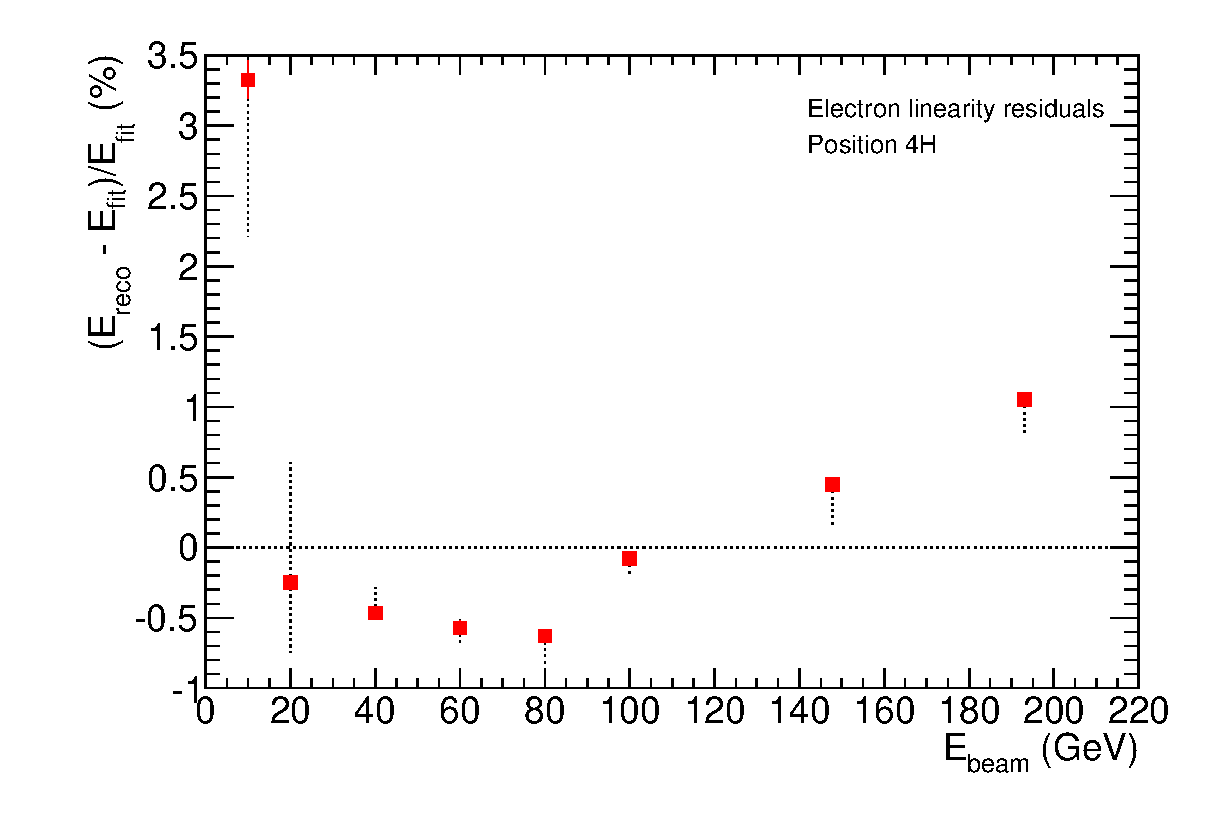
\includegraphics[width=0.95\linewidth,angle=0]{FCalTB_plots/electron_residuals_4H_data.eps}
%\end{center}
%\caption{Residuals obtained from the linearity fit for electrons at position 4H. Solid lines in the error bars represent the statistical uncertainties, while the systematic uncertainties are represented by the dotted lines. }
%\label{TBplot_electron_residuals_4H}
%\end{figure}
%%%%%%%%%%%%%%%%%%%%%%%%%%%%%%%%%%%%%%%%%%%%%%%%%%%%%%%%%%%%%%%%
%
%%%%%%%%%%%%%%%%%%%%%%%%%%%%%%%%%%%%%%%%%%%%%%%%%%%%%%%%%%%%%%%%
%\begin{figure}[!htb]
%\begin{center}
%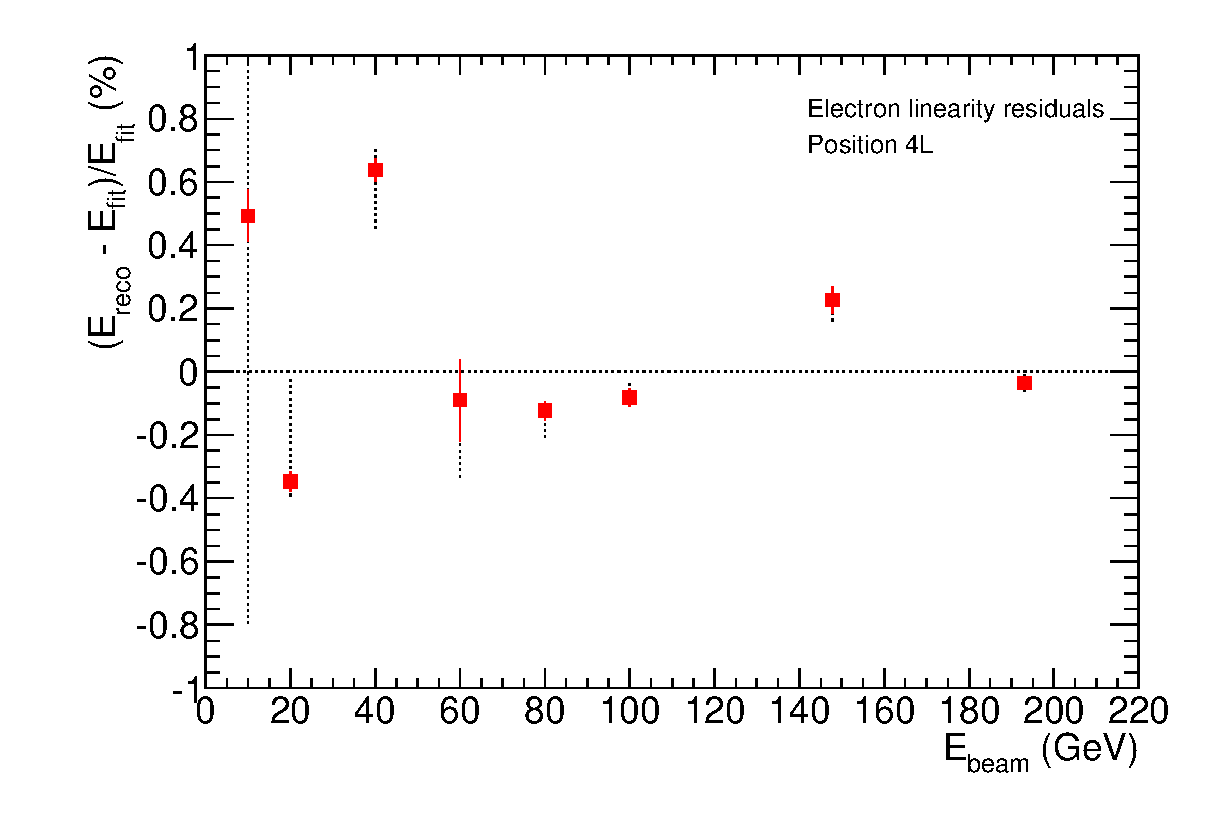
\includegraphics[width=0.95\linewidth,angle=0]{FCalTB_plots/electron_residuals_4L_data.eps}
%\end{center}
%\caption{Residuals obtained from the linearity fit for electrons at position 4L. Solid lines in the error bars represent the statistical uncertainties, while the systematic uncertainties are represented by the dotted lines. }
%\label{TBplot_electron_residuals_4L}
%\end{figure}
%%%%%%%%%%%%%%%%%%%%%%%%%%%%%%%%%%%%%%%%%%%%%%%%%%%%%%%%%%%%%%%%
%%%%%%%%%%%%%%%%%%%%%%%%%%%%%%%%%%%%%%%%%%%%%%%%%%%%%%%%%%%%%%%
\begin{figure}[htb]
\begin{center}
\subfigure[]{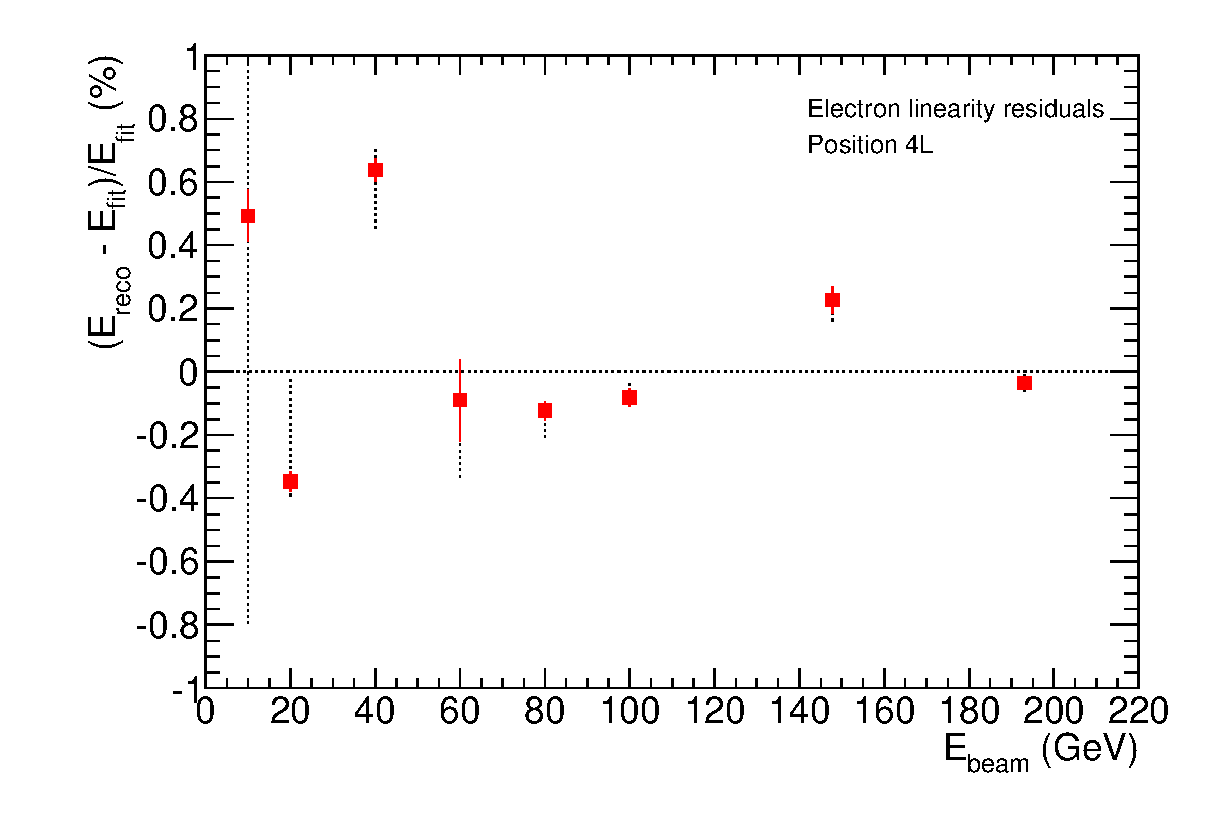
\includegraphics[width=0.45\linewidth,angle=0]{FCalTB_plots/electron_residuals_4L_data.eps}
\label{TBplot_electron_residuals_4L}}
\subfigure[]{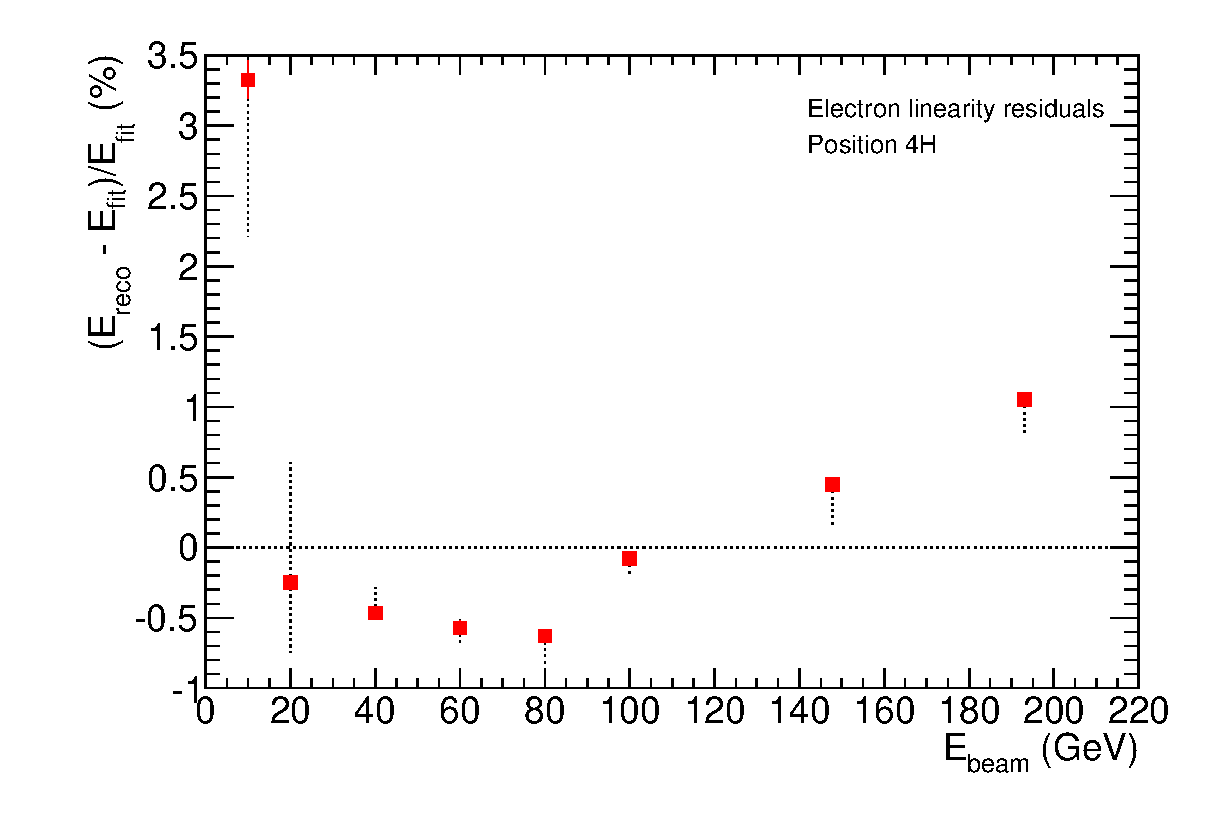
\includegraphics[width=0.45\linewidth,angle=0]{FCalTB_plots/electron_residuals_4H_data.eps}
\label{TBplot_electron_residuals_4H}}
\end{center}
\caption{Residuals obtained from the linearity fit for electrons at position 4L (left) and 4H (right). Solid lines in the error bars represent the statistical uncertainties, while the systematic uncertainties are represented by the dotted lines. }
\label{TBplot_electron_residuals}
\end{figure}
%%%%%%%%%%%%%%%%%%%%%%%%%%%%%%%%%%%%%%%%%%%%%%%%%%%%%%%%%%%%%%%



The energy resolution of the FCal response to electrons is plotted in Figure~\ref{TBplot_electron_resolution}, for both data and simulation results. As the randomly triggered events provide information on the amount of noise present in the electronics, the contribution of this noise has been subtracted in quadrature from the width of the response. The resolution is thus defined as $\sigma_E/\overline{E}$, where
\begin{equation}
\sigma_E = \sqrt{\sigma^2 - \sigma_N^2}
\end{equation}
where $\sigma_N$ is the width of the noise distribution reconstructed from randomly triggered events. The width of the electron peak, $\sigma$, and the mean response, $\overline{E}$, are obtained from the double Gaussian fit as described by equations~\ref{DG_width_def} and \ref{eqn_moment}. The values of these quantities are listed in in Tables~\ref{TBres_table_elec_4L} and \ref{TBres_table_elec_4H}, for position 4L and position 4H, respectively. As noted earlier, the amount of noise present in the electronics varied over time, but was generally around 14-17 ADC counts (1.2-1.4 GeV). The RMS of the noise contribution to the cluster energy has been plotted as a function of beam energy in Figure~\ref{TBplot_noisevbeam_electrons}.


The resolution is fit to a function of the form
\begin{equation}
%\frac{\sigma_E}{E} = \left ( \frac{A^2}{E/GeV} + B^2\right )^{\frac{1}{2}},
\frac{\sigma_E}{\overline{E}} = \frac{A}{\sqrt{E}} \oplus B
\label{resolution_fit_equation}
\end{equation}
where $A$ is the called the stochastic term, and represents the contribution to the resolution arising from fluctuations in the energy deposited in the liquid argon gaps of the FCal. The constant term, $B$, is due to effects that are independent of the beam energy, such as non-uniformities in the calorimeter structure or energy leakage. A term proportional to $E^{-2}$ is sometimes included in equation~\ref{resolution_fit_equation} to describe the effects of noise on the resolution. However, as the noise present in the testbeam electronics was observed to vary over time, it is not appropriate to parameterize it in this way. Instead, the noise is dealt with by the subtraction procedure described earlier, and so a noise term is not included in equation ~\ref{resolution_fit_equation}. The fit results are listed in Table~\ref{table_resolution_electrons}.


\begin{table}[!htb]
\begin{center}
\begin{tabular}{|l|l|l|l|}
\hline
& Stochastic Term (\% $\mathrm{GeV}^{1/2}$) & Constant Term (\%) \\
\hline
Data (4L) & 27.0 $\pm$ 0.2 & 3.58 $\pm$ 0.02\\
Simulation (4L) & 24.7 $\pm$ 0.3 & 4.56 $\pm$ 0.03\\
Data (4H) & 33.7 $\pm$ 0.2 & 3.11 $\pm$ 0.03\\
Simulation (4H) & 28.1 $\pm$ 0.3 & 3.96 $\pm$ 0.03\\
\hline
\end{tabular}
\end{center}
\caption{Fit parameters for energy resolution to electrons. Quoted uncertainties are statistical only.}
\label{table_resolution_electrons}
\end{table}


\begin{figure}[htb]
\begin{center}
\subfigure[]{\includegraphics[width=0.45\linewidth,angle=0]{FCalTB_plots/electron_resolution_4L.eps}
\label{TBplot_electron_resolution_4L}}
\subfigure[]{\includegraphics[width=0.45\linewidth,angle=0]{FCalTB_plots/electron_resolution_4H.eps}
\label{TBplot_electron_resolution_4H}}
\caption{Energy resolution of the FCal to electrons, using data taken from position 4L (left) and 4H (right). A noise subtraction procedure has been applied, as described in the text.}
\label{TBplot_electron_resolution}
\end{center}
\end{figure}
%%%%%%%%%%%%%%%%%%%%%%%%%%%%%%%%%%%%%%%%%%%%%%%%%%%%%%%%%%%%%%%

%%%%%%%%%%%%%%%%%%%%%%%%%%%%%%%%%%%%%%%%%%%%%%%%%%%%%%%%%%%%%%%
\begin{figure}[htb]
\begin{centering}
\subfigure{
\includegraphics[width=0.45\linewidth,angle=0]{FCalTB_plots/Electron_response_4L_data_noisevbeam.eps}
\label{TBplot_noisevbeam_4L}
}
\subfigure{

\includegraphics[width=0.45\linewidth,angle=0]{FCalTB_plots/Electron_response_4H_data_noisevbeam.eps}
\label{TBplot_noisevbeam_4H}
}
\caption{RMS of the electronics noise clustered at different energies, for electron beams directed at position 4L (left) and position 4H (right).  } 
\label{TBplot_noisevbeam_electrons}
\end{centering}
\end{figure}

%%%%%%%%%%%%%%%%%%%%%%%%%%%%%%%%%%%%%%%%%%%%%%%%%%%%%%%%%%%%%%%



The non-uniformity of the response with respect to the beam particle impact point on the calorimeter forms the dominant contribution to the constant term in the resolution \cite{TB98_electron_signals}. The additional upstream material present for runs directed at position 4H can cause the beam particles to begin showering earlier. The energy in the shower is thus distributed over a larger area by the time it reaches the FCal, decreasing the impact point dependence and resulting in a lower constant term for the resolution measured at position 4H. The simulation results for electrons give a higher (i.e. worse) resolution than that seen in data, although the discrepancy is smaller at position 4H than 4L. Again, the effects of the additional material at position 4H are well modelled by the simulation. The constant term at position 4L is 15\% higher than that seen at 4H, in both data and simulation.

The sources of systematic uncertainty considered for the electron energy resolution are the same as those  considered for the response linearity. Again, the systematic uncertainties are dominated by beam energy fluctuations and the choice of cluster size, with other effects providing a smaller contribution. The resolution at position 4L is best described by a stochastic term of (27.0 $\pm \, 0.9) \% \cdot (\mathrm{GeV})^{1/2}$ and a constant term of (3.58 $\pm \, 0.09) \%$, while the reolution at position 4H is best described by a stochastic term of (33.7 $\pm 0.8) \% \cdot (\mathrm{GeV})^{1/2}$ and a constant term of (3.11 $\pm 0.09) \%$. These uncertainties are again dominated by systematic effects, with the statistical uncertainties being listed in Table~\ref{table_resolution_electrons}.

The resolution at 4L presented here has a stochastic term of 27.0\%$ \cdot \surd{GeV}$, which is slightly lower than the published result of 28.5 \%$ \cdot \surd{GeV}$ \cite{Fcalpaper}. This difference is due to the rounding error discussed in section~\ref{TBoverview_offline}, which has been corrected in these results but was undiscovered at the time of publication. The constant term presented here (3.58\%) is slightly larger than the published value (3.5\%), but these values are consistent within the uncertainties. 
%The agreement between data and Monte Carlo is generally good, a


%\red{FIXFIXFIXFIXFIX systematics on electron resolution}



\cmt{ DONE WITH ELECTORNS WOOOOOO}


%The response of the FCal to electrons directed at position 4L is shown in Figure~\ref{TBplot_electron_response_4L_data}. A beam particle that strikes the calorimeter in the centre of an electrode rod, or in the middle of the absorber, will have a produce a smaller response than a particle that impacts close to the liquid argon gap. As the beamspot has a diameter of 65 mm, which is much greater than the spacing between electrodes (7.5 mm in FCal1), the collected data is derived from many different impact points. 



%geometry-impact point dependence
%double Gaussian used - mean and width taken from the fit
%describe moment calculation used for error in width, mean, etc.
%fit and mean given by 
%6 parameter fit used at 200~GeV, ratio of peak means and populations obtained, used when fitting lower energies - skip this
%
%Results - mean/width Table


%systematic errors - discuss here before linearity stuff.
%Polarity effects.
%
%
%linearity plot, and residuals
%
%
%discussion of linearity,  systematic errors
%- 4L slope of 12.0, agrees with the SPICE simulation.
%intercept allowed to vary, in order to account for upstream material losses.
%c.f. MC - indicates that there is some material not modeled in MC (such as upstream of B9)
%
%
%
%effect of systematics estimated by varying stuff, fitting, and obtaining linearity. systematic uncertainty in slope taken as mac deviation of varied data from nominal analysis.,same for intercept. 
%
%
%
%Noise plot - For each event, a randomly triggered event chosen from the same run. The same channels that are clustered in the "physics" event are summed in the randomly triggered event. In this way a distribution of the clustered noise can be built up, 
%
%Resolution plot
%
%Resolution - noise subtraction method
%
%systematics
%
%quote numbers.













%event selection
%-triggering, scintillators, etc
%-beam cleaning/envelope cuts
%-veto counter
%-timing
%-CEDAR

%analysis
%8cm clustering - relate to moliere radius, XX\% of the energy should be contained (Wigmans)
%response fitting - double Gaussian, impact point dependence
%linearity
%- SPICE predictions of 12.0~GeV/ADC
%- floating intercept - dead material upstream (CEDAR)
%- systematic uncertainties - polarity, clustering
%
%
%comparison between 4L and 4H, data and MC
%
%
%resolution - noise subtraction
%systematics
%
%comparison between 4L and 4H, data and MC
%
%plots - electron response at 4L
%
%
\clearpage

\subsection{Analysis of Hadron Data}
%event selection
%- same as for electrons, but with beam envelope oriented at pions
%- CEDAR

%do radial/ longitudinal profiles first, EM scale.
%weights, weight derivation

%response, linearity, resolution, etc.

%beams of pi+ and pi-. 
%Event selection for hadrons is the same as that for electrons, although the CEDAR cut is applied for $\pi+$ beams at all energies below 200GeV in order to reduce the amount of proton contamination. \blue{halflings}. 

In the analysis of hadron data, the signal from the FCal is first calibrated to the electromagnetic (EM) scale. This is done by applying ADC2MeV factors, which convert the reconstructed pulse peak (in ADC counts) to the corresponding energy deposited in the calorimeter by an electromagnetic particle (i.e. an electron or photon). For the beam test, the ADC2MeV values used to reconstruct signals from the FCal are 83.3 MeV/ADC for FCal1, 163.9 MeV/ADC for FCal2 and 185.2 MeV/ADC for  FCal3. These are the same values used in the published analysis\cite{FCal_paper}, which were originally obtained from a SPICE simulation of the FCal electronics. As discussed above, the predicted value for FCal1 is in good agreement with the value obtained from the linearity of the FCal1 response to electrons. During a previous beam test\cite{TB98_electron_signals}, the response to electrons was studied for prototypes of the FCal1 and FCal2 modules. The ratio of these responses was measured from this data, and used to validate the SPICE predictions for the EM scale factors of the hadronic modules.

%Data taken in a previous beam test \cite{TB98_electron_signals} studied
%
% allowed the ratio of the FCal1 and FCal2 responses to electrons to be studied, and the SPICE results agree with this data to within 5\%.
%\red{fix this}
%\red{CITE THIS}.


%here are the radial profiles and longitudinal profiles, at the EM scale
% %%%%%%%%%%%%%%%%%%%%%%%%%%%%%%%%%%%%%%%%%%%%%%%%%%%%%%%%%%%%%%%
\begin{figure}[!htb]
\begin{center}

\subfigure[]{
\includegraphics[width=0.45\linewidth,angle=0]{FCalTB_plots/pions_4L_radial_int.eps}
\label{pion_radial_4L_int}
}
\subfigure[]{
\includegraphics[width=0.45\linewidth,angle=0]{FCalTB_plots/pions_4L_radial_diff.eps}
\label{pion_radial_4L_diff}
} \\
%\caption{Energy distribution within the FCal as a function of the transverse distance ($r$) from the projected beam impact point. Figure~\ref{pion_radial_4L_diff} shows the differential energy distribution while Figure~\ref{pion_radial_4L_int} shows the cumulative distribution. }
%\label{TBplot_radial_profiles_4L}
\subfigure[]{
\includegraphics[width=0.45\linewidth,angle=0]{FCalTB_plots/pions_4H_radial_int.eps}
\label{pion_radial_4H_int}
}
\subfigure[]{
\includegraphics[width=0.45\linewidth,angle=0]{FCalTB_plots/pions_4H_radial_diff.eps}
\label{pion_radial_4H_diff}
}
\caption{Energy distribution within the FCal as a function of the transverse distance ($r$) from the projected beam impact point. Results obtained from position 4L are shown in the upper row, while results from position 4H are in the lower row. Figures~\ref{pion_radial_4H_int} and \ref{pion_radial_4L_int} shows the cumulative energy distribution while Figures~\ref{pion_radial_4L_diff} and \ref{pion_radial_4H_diff} show the derivatives of these plots. }
\label{TBplot_radial_profiles}
\end{center}
\end{figure}
%%%%%%%%%%%%%%%%%%%%%%%%%%%%%%%%%%%%%%%%%%%%%%%%%%%%%%%%%%%%%%%

Figure~\ref{TBplot_radial_profiles} shows the transverse distribution of energy (at the EM scale) for 200~GeV hadrons showering within the FCal, for beams directed at position 4L and 4H.. \cmt{The projected beam impact point for each module is derived from the tracking information.} 

Figures~\ref{pion_radial_4L_int} and \ref{pion_radial_4H_int} show the energy deposited within a transverse distance $r$ from the impact point. These plots show the integrated energy contained within a cylinder of radius $r$ centred on the impact point, normalised to the energy contained within a cylinder of radius 21cm\footnote{Any energy that propagates (transversely) further than 21cm from the centre of the beamspot is not contained within the FCal. It is either lost beyond the outer diameter of the FCal modules or leaks into the hole at the centre of the FCal.}. As the FCal is oriented at an angle of $2.98^\circ$ with respect to the beam line, an impact point is calculated for each module by projecting the particle track through the calorimeter. The simulation results (for all physics lists studied) show that a slightly larger fraction of the energy is contained within smaller transverse distances, indicating that the simulated showers are narrower than those observed in data. This is consistent with other \atlas simulation results\cite{CTB_localHadCal,calpub2010}. Cylindrical clusters of radius 16cm are used for analysis of the hadron data, which contain $\sim 99\%$ of the energy deposited in the calorimeter. 

Figures~\ref{pion_radial_4L_diff} and \ref{pion_radial_4H_diff} depict the rate at which energy is deposited as a function of $r$, showing in detail the energy deposited at small radii. Each bin shows the amount of energy contained within a cylindrical shell of thickness 0.5cm, again shown as a fraction of the total energy contained within a cylinder of radius 21cm. 


%%%%%%%%%%%%%%%%%%%%%%%%%%%%%%%%%%%%%%%%%%%%%%%%%%%%%%%%%%%%%%%%
%\begin{figure}[!htb]
%\begin{center}
%\subfigure[]{
%\includegraphics[width=0.45\linewidth,angle=0]{FCalTB_plots/pions_4L_radial_diff.eps}
%\label{pion_radial_4L_diff}
%}
%\subfigure[]{
%\includegraphics[width=0.45\linewidth,angle=0]{FCalTB_plots/pions_4L_radial_int.eps}
%\label{pion_radial_4L_int}
%}
%\caption{Energy distribution within the FCal as a function of the transverse distance ($r$) from the projected beam impact point. Figure~\ref{pion_radial_4L_diff} shows the differential energy distribution while Figure~\ref{pion_radial_4L_int} shows the cumulative distribution. }
%\label{TBplot_radial_profiles_4L}
%\end{center}
%\end{figure}
%%%%%%%%%%%%%%%%%%%%%%%%%%%%%%%%%%%%%%%%%%%%%%%%%%%%%%%%%%%%%%%%
%
%%%%%%%%%%%%%%%%%%%%%%%%%%%%%%%%%%%%%%%%%%%%%%%%%%%%%%%%%%%%%%%%
%\begin{figure}[!htb]
%\begin{center}
%\subfigure[]{
%\includegraphics[width=0.45\linewidth,angle=0]{FCalTB_plots/pions_4H_radial_diff.eps}
%\label{pion_radial_4H_diff}
%}
%\subfigure[]{
%\includegraphics[width=0.45\linewidth,angle=0]{FCalTB_plots/pions_4H_radial_int.eps}
%\label{pion_radial_4H_int}
%}
%\caption{Energy distribution within the FCal as a function of the transverse distance ($r$) from the projected beam impact point. Figure~\ref{pion_radial_4H_diff} shows the differential energy distribution while Figure~\ref{pion_radial_4H_int} shows the cumulative distribution. }
%\label{TBplot_radial_profiles_4L}
%\end{center}
%\end{figure}
%%%%%%%%%%%%%%%%%%%%%%%%%%%%%%%%%%%%%%%%%%%%%%%%%%%%%%%%%%%%%%%%
 %%%%%%%%%%%%%%%%%%%%%%%%%%%%%%%%%%%%%%%%%%%%%%%%%%%%%%%%%%%%%%%

The longitudinal shower profiles for 200~GeV hadrons are shown in Figure~\ref{TBplot_long_profiles}. These show the amount of energy (at the EM scale) clustered within each module as a fraction of the total energy clustered in all modules. The simulation  results show more energy deposited in FCal1 and less energy in FCal2, indicating the the simulated showers are shorter than those observed in data. This is also consistent with other \atlas simulation results\cite{calpub2010}.

The shower maximum is the longitudinal depth at which the particle shower contains the largest number of particles, and thus corresponds to the depth at which the energy deposition is greatest. The additional material in front of position 4H causes the shower to start earlier, and thus moves the location of the shower maximum back towards the front of the FCal. This results in a larger fraction of energy being deposited in FCal1 at position 4H compared to position 4L.


%
%% shower max  ~~1.76 \lambda int at 200~GeV
%16 cm cluster
%EM scale energy vs beam energy
%
%hadronic showers/calibration
%


%
%16 cm cluster used, reconstructed energy plotted here, at EM scale Energy clustered in each module, rather than just FCal1. 
%
%Higher energy the EM component of the shower increases, hence the plot for hadrons is not linear, as it is in Figure~\ref{}. ADc2GeV factors. 12.0 seen in electron analysis, ratio of alpha2 to alpha1 obtained from 98 testbeam, which used a prototype of the FCal. 
%%%%%%%%%%%%%%%%%%%%%%%%%%%%%%%%%%%%%%%%%%%%%%%%%%%%%%%%%%%%%%%
\begin{figure}[!htb]
\begin{center}
\subfigure[]{\includegraphics[width=0.45\linewidth,angle=0]{FCalTB_plots/pions_4L_long.eps}
\label{TBplot_long_profile_4L}}
%\caption{Longitudinal distribution of energy deposited in the FCal, for 200GeV hadrons directed at position 4L.}
\subfigure[]{\includegraphics[width=0.45\linewidth,angle=0]{FCalTB_plots/pions_4H_long.eps}
\label{TBplot_long_profile_4H}}
\caption{Longitudinal distributions of energy deposited in the FCal. These show the relative amounts of energy clustered in each module, for beams directed at position 4L (left) and 4H (right).}
\label{TBplot_long_profiles}
\end{center}
\end{figure}
%%%%%%%%%%%%%%%%%%%%%%%%%%%%%%%%%%%%%%%%%%%%%%%%%%%%%%%%%%%%%%%


%%%%%%%%%%%%%%%%%%%%%%%%%%%%%%%%%%%%%%%%%%%%%%%%%%%%%%%%%%%%%%%%
%\begin{figure}[!htb]
%\begin{center}
%\includegraphics[width=0.8\linewidth,angle=0]{FCalTB_plots/pions_4L_long.eps}
%\end{center}
%\caption{Longitudinal distribution of energy deposited in the FCal, for 200GeV hadrons directed at position 4L.}
%\label{TBplot_long_profile_4L}
%\end{figure}
%%%%%%%%%%%%%%%%%%%%%%%%%%%%%%%%%%%%%%%%%%%%%%%%%%%%%%%%%%%%%%%%
%
%
%
%%%%%%%%%%%%%%%%%%%%%%%%%%%%%%%%%%%%%%%%%%%%%%%%%%%%%%%%%%%%%%%%
%\begin{figure}[!htb]
%\begin{center}
%\includegraphics[width=0.8\linewidth,angle=0]{FCalTB_plots/pions_4H_long.eps}
%\end{center}
%\caption{Longitudinal distribution of energy deposited in the FCal, for 200GeV hadrons directed at position 4H.}
%\label{TBplot_long_profile_4H}
%\end{figure}
%%%%%%%%%%%%%%%%%%%%%%%%%%%%%%%%%%%%%%%%%%%%%%%%%%%%%%%%%%%%%%%%

% A feature of hadronic showers is that not all of the shower's energy is visible to the calorimeter. For example, when a nucleus breaks up as a result of an interaction with a showering hadron, an amount of nuclear binding energy is lost from the products of the reaction. Alternatively, hadronic interactions may lead to the production of a neutrino, which will carry energy out of the detector. Muons may also be produced in hadronic showers, which will deposit a minimal amount of energy in the active regions before leaving the calorimeter. Energy lost in processes such as these cannot be measured by the calorimeter, resulting in a response lower than that seen for an EM particle with the same energy \footnote{Compensating calorimeters (such as ZEUS\cite{zeus_detector}) are designed to correct for this effect, such that the response to hadrons will be equal to that for electrons of the same energy.}. For this reason, the energy reconstructed at the EM scale is some fraction of the energy of the incident hadron, typically around 60-80\% for the beam energies considered in this analysis.
 
 
The mean response of the FCal to hadrons is plotted in Figure~\ref{hadron_linearity_EMc16}, as a function of the beam energy. The response here is again taken at the EM scale.
Some particles produced in hadronic interactions, such as $\eta$ and $\pi^0$ mesons, decay to photons which then shower electromagnetically.  Hadronic showers thus have an EM component, and the relative amount of the shower energy that is carried by this EM component increases with the energy of the initial hadron \cite{wigmans2000calorimetry}. This EM component tends to be contained close to the shower axis, giving hadronic showers a narrow EM ``core''. This feature of hadronic showers gives rise to the nonlinear behaviour seen in Figure~\ref{hadron_linearity_EMc16}: as the beam energy increases, the EM component of the shower also increases, giving a higher response at the EM scale.

%The mean response of the FCal to hadrons is plotted in Figure~\ref{hadron_linearity_EMc16}, as a function of the beam energy. The response here is again taken at the EM scale.

% It is this behaviour that gives rise to the non-linear shape seen in Figure ~\ref{hadron_linearity_EMc16}.
%Showering hadrons may 
%
%Not all energy of a hadronic shower is visible 
%
%EM and non-EM components
%
%
%
%
%
%
%The energy in a hadronic shower is carried by an EM component and a non-EM component. 
%
%not all energy visible, Em component and hadronic component. Not all of the energy in the hadronic component is visible, 
%
% Hadronic showers deposit less vis


%%%%%%%%%%%%%%%%%%%%%%%%%%%%%%%%%%%%%%%%%%%%%%%%%%%%%%%%%%%%%%%
\begin{figure}[!htb]
\begin{centering}
\subfigure[]{
\includegraphics[width=0.45\linewidth,angle=0]{FCalTB_plots/hadron_linearity_4L_EMscale.eps}
\label{hadron_linearity_EMc16_4L}
}
\subfigure[]{
\includegraphics[width=0.45\linewidth,angle=0]{FCalTB_plots/hadron_linearity_4H_EMscale.eps}
\label{hadron_linearity_EMc16_4H}
}
\caption{Ratio of energy reconstructed at the EM scale to the beam energy, for hadrons directed at position 4L (left) and 4H (right).} 
\label{hadron_linearity_EMc16}
\end{centering}
\end{figure}




The measured EM scale energy may be calibrated to the hadronic scale through a flat weighting scheme, whereby a single weight is assigned to each module. The calibrated energy is then given by 
%Hadronic calibration is accomplished through a flat weighting scheme, whereby a single weight is assigned to each module. reconstructed energy then given by

\begin{equation}
E_\mathrm{reco} = g_1 E_1^\mathrm{EM} +  g_2 E_2^\mathrm{EM} +  g_3 E_3^\mathrm{EM}
\end{equation}
 where $E_1^\mathrm{EM}$, $E_2^\mathrm{EM}$, and $E_3^\mathrm{EM}$ are the EM scale energies clustered in FCal1, FCal2 and FCal3, respectively,  and $g_1$, $g_2$, and $g_3$ are the flat weights for these modules.
%  is the flat weight associated with the $i$-th FCal module, and $E_i^\mathrm{EM}$ is the EM scale energy clustered in this module.
 
 
 
The weights are derived at a given beam energy, as energy dependent weights can not be used at ATLAS. They are obtained by minimising the function
\begin{equation}
\chi^2 = \sum_i^{N_\mathrm{events}}\left( g_1 E_{1,i}^\mathrm{EM} +  g_2 E_{2,i}^\mathrm{EM} +  g_3 E_{3,i}^\mathrm{EM} - E_\mathrm{beam} \right )^2
\label{weight_chi2}
\end{equation}
where $E_\mathrm{beam}$ is the beam energy and the sum  runs over all events taken at this energy. The weights are constrained such that the mean reconstructed energy is equal to the beam energy. This constraint is implemented by assigning $g_3$ the value
\begin{equation}
\label{hadronic_weight_constraint}
g_3 = \frac{ E_\mathrm{beam}  - g_1 \langle E_{1}^\mathrm{EM}\rangle - g_2 \langle E_{2}^\mathrm{EM}\rangle }{\langle E_{3}^\mathrm{EM}\rangle},
\end{equation}
where the angled brackets denote the average taken over all events. With this constraint applied, the $\chi^2$ in equation~\ref{weight_chi2} becomes equal to the variance of the reconstructed energy, and so minimising $\chi^2$ minimises the width of the distribution of reconstructed energy.


\begin{figure}
\begin{center}
\subfigure[]{
\includegraphics[width=0.45\linewidth,angle=0]{FCalTB_plots/weightfigs/weights_4L_c16_g1.eps}
\label{weight_c16_4L1}
}
\subfigure[]{
\includegraphics[width=0.45\linewidth,angle=0]{FCalTB_plots/weightfigs/weights_4H_c16_g1.eps}
\label{weight_c16_4H1}
}
\\
\subfigure[]{
\includegraphics[width=0.45\linewidth,angle=0]{FCalTB_plots/weightfigs/weights_4L_c16_g2.eps}
\label{weight_c16_4L2}
}
\subfigure[]{
\includegraphics[width=0.45\linewidth,angle=0]{FCalTB_plots/weightfigs/weights_4H_c16_g2.eps}
\label{weight_c16_4H2}
}
\\
\subfigure[]{
\includegraphics[width=0.45\linewidth,angle=0]{FCalTB_plots/weightfigs/weights_4L_c16_g3.eps}
\label{weight_c16_4L3}
}
\subfigure[]{
\includegraphics[width=0.45\linewidth,angle=0]{FCalTB_plots/weightfigs/weights_4H_c16_g3.eps}
\label{weight_c16_4H3}
}
\caption{Flat weights used in hadronic calibration, as a function of the energy at which they are derived. Only the weights derived using 200GeV are used in the analysis.  }
\label{TBplot_c16_weights}
\end{center}
\end{figure}

The flat weights derived at each energy are plotted in Figures~\ref{weight_c16}, for beams directed at position 4L (a,c,e) and 4H (b,d,f). Weights derived using Monte Carlo results are also shown for comparison, but are not used in the analysis: weights derived from 200~GeV data are used to calibrate all data and simulation results to the hadronic scale. As the beam energy decreases the relative amount of energy deposited in FCal1 and FCal2 increases, while that deposited in FCal3 decreases. Consequently, the weights $g_1$ and $g_2$ increase with decreasing beam energy, while $g_3$ decreases. At 10~GeV the relative amount of energy deposited in FCal2 drops abruptly, resulting in large increase of $g_1$ and a sudden drop in $g_2$.  The uncertainty on $g_3$ is found by propagating the statistical uncertainties on $g_1$ and $g_2$. As FCal3 contains only a small fraction of the total energy deposited in the FCal, even at highest beam energies available during the beam test, this results in an uncertainty on $g_3$ that is much larger than the uncertainties on the other two weights.


 % behaviour of weights, 4H vs 4L

%energy dependent weights at ATLAS?

%The hadronic response of the FCal is plotted in Figures~\ref{TBplot_hadron response_4L_data} (4L) and \ref{TBplot_hadron response_4L_data} (4H)

%\newline
\vspace{0.3cm}

The response of the FCal to hadron beams of various energies is plotted in Figure~\ref{TBplot_hadron_response_4L_data} for position 4L and Figure~\ref{TBplot_hadron_response_4H_data} for position 4H. The responses obtained from simulation  are shown in appendix~\ref{appendix_MCresults}, for all three of the physics lists considered. A double Gaussian is fitted to the response and used to extract the mean and width, as was done in the electron analysis. The results obtained from the fitting are summarised in Tables~\ref{TBres_table_hadron_4L} and ~\ref{TBres_table_hadron_4H}. The statistical uncertainties associated with the hadronic weights have been neglected here. When the weights $g_1$ and $g_2$ are varied by their uncertainties and $g_3$ is subsequently determined by the constraint (equation~\ref{hadronic_weight_constraint}), the observed variation in the fit results is negligible. The noise contribution to the clustered energy was estimated from randomly triggered events, using the same method as the electron analysis. This is plotted as a function of beam energy in Figure~\ref{TBplot_hadron_noisevbeam}.

%%%%%%%%%%%%%%%%%%%%%%%%%%%%%%%%%%%%%%%%%%%%%%%%%%%%%%%%%%%%%%%
\begin{table}[!htb]
\begin{center}
\begin{tabular}{|l|l|l|l|}
\hline
Beam Energy (GeV) & Fitted Mean (GeV)& Fitted Width (GeV)& Noise (GeV) \\
\hline
%200 GeV  &   200.1 $\pm$     0.1 &    19.5 $\pm$     0.0 &     6.4 $\pm$     0.0 \\
%150 GeV  &   148.4 $\pm$     0.0 &    16.1 $\pm$     0.0 &     6.5 $\pm$     0.0 \\ %old
%120 GeV  &   118.3 $\pm$     0.0 &    14.2 $\pm$     0.0 &     6.8 $\pm$     0.0 \\
%100 GeV  &    97.7 $\pm$     0.1 &    13.4 $\pm$     0.1 &     7.3 $\pm$     0.0 \\
% 80 GeV  &    77.3 $\pm$     0.1 &    11.3 $\pm$     0.0 &     6.5 $\pm$     0.0 \\
% 60 GeV  &    56.7 $\pm$     0.0 &     9.6 $\pm$     0.0 &     6.1 $\pm$     0.0 \\
% 40 GeV  &    37.2 $\pm$     0.1 &     8.5 $\pm$     0.1 &     6.1 $\pm$     0.0 \\
% 10 GeV  &     8.2 $\pm$     0.1 &     6.6 $\pm$     0.1 &     6.2 $\pm$     0.1 \\
200 GeV  &  200.08 $\pm$    0.06 &   19.46 $\pm$    0.04 &    6.41 $\pm$    0.01 \\
150 GeV  &  148.39 $\pm$    0.04 &   16.05 $\pm$    0.03 &    6.55 $\pm$    0.01 \\
120 GeV  &  118.27 $\pm$    0.05 &   14.24 $\pm$    0.03 &    6.76 $\pm$    0.02 \\
100 GeV  &   97.6 $\pm$    0.1 &   13.37 $\pm$    0.08 &    7.29 $\pm$    0.05 \\
80 GeV  &   77.29 $\pm$    0.06 &   11.31 $\pm$    0.04 &    6.53 $\pm$    0.03 \\
60 GeV  &   56.74 $\pm$    0.03 &    9.59 $\pm$    0.02 &    6.08 $\pm$    0.01 \\
40 GeV  &   37.2 $\pm$    0.1 &    8.49 $\pm$    0.07 &    6.12 $\pm$    0.05 \\
10 GeV  &    8.2 $\pm$    0.1 &    6.60 $\pm$    0.08 &    6.17 $\pm$    0.08 \\
\hline
\end{tabular}
\end{center}
\caption{Results for the FCal response to hadrons directed at position 4L. Quoted errors are statistical only.}
\label{TBres_table_hadron_4L}
\end{table}
%%%%%%%%%%%%%%%%%%%%%%%%%%%%%%%%%%%%%%%%%%%%%%%%%%%%%%%%%%%%%%%
%%%%%%%%%%%%%%%%%%%%%%%%%%%%%%%%%%%%%%%%%%%%%%%%%%%%%%%%%%%%%%%
\begin{table}[!htb]
\begin{center}
\begin{tabular}{|l|l|l|l|}
\hline
Beam Energy (GeV) & Fitted Mean (GeV)& Fitted Width (GeV)& Noise (GeV) \\
\hline
%200 GeV  &   201.0 $\pm$     0.1 &    23.4 $\pm$     0.0 &     6.5 $\pm$     0.0 \\ %old
%150 GeV  &   149.5 $\pm$     0.1 &    19.1 $\pm$     0.1 &     6.4 $\pm$     0.0 \\
%120 GeV  &   118.4 $\pm$     0.1 &    17.1 $\pm$     0.0 &     7.2 $\pm$     0.0 \\
%100 GeV  &    97.5 $\pm$     0.1 &    15.9 $\pm$     0.1 &     7.6 $\pm$     0.0 \\
% 80 GeV  &    76.7 $\pm$     0.1 &    14.1 $\pm$     0.0 &     7.6 $\pm$     0.0 \\
% 60 GeV  &    56.1 $\pm$     0.0 &    11.7 $\pm$     0.0 &     6.7 $\pm$     0.0 \\
% 40 GeV  &    36.1 $\pm$     0.1 &     9.9 $\pm$     0.1 &     6.5 $\pm$     0.1 \\
% 10 GeV  &     7.0 $\pm$     0.1 &     7.2 $\pm$     0.1 &     6.4 $\pm$     0.1 \\
200 GeV  &  200.95 $\pm$    0.07 &   23.41 $\pm$    0.05 &    6.46 $\pm$    0.01 \\
150 GeV  &  149.26 $\pm$    0.05 &   19.20 $\pm$    0.03 &    6.46 $\pm$    0.01 \\
120 GeV  &  118.35 $\pm$    0.05 &   17.10 $\pm$    0.04 &    7.13 $\pm$    0.02 \\
100 GeV  &   97.5 $\pm$    0.1 &   15.88 $\pm$    0.07 &    7.63 $\pm$    0.03 \\
80 GeV  &   76.73 $\pm$    0.06 &   14.12 $\pm$    0.04 &    7.60 $\pm$    0.02 \\
60 GeV  &   56.14 $\pm$    0.03 &   11.73 $\pm$    0.02 &    6.70 $\pm$    0.01 \\
40 GeV  &   36.1 $\pm$    0.1 &    9.93 $\pm$    0.09 &    6.47 $\pm$    0.06 \\
10 GeV  &    7.0 $\pm$    0.1 &    7.23 $\pm$    0.08 &    6.39 $\pm$    0.07 \\
\hline
\end{tabular}
\end{center}
\caption{Results for the FCal response to hadrons directed at position 4H. Quoted errors are statistical only.}
\label{TBres_table_hadron_4H}
\end{table}
%%%%%%%%%%%%%%%%%%%%%%%%%%%%%%%%%%%%%%%%%%%%%%%%%%%%%%%%%%%%%%%
%%%%%%%%%%%%%%%%%%%%%%%%%%%%%%%%%%%%%%%%%%%%%%%%%%%%%%%%%%%%%%%%
%\begin{figure}[!htb]
%\begin{center}
%\includegraphics[width=1.0\linewidth,angle=0]{FCalTB_plots/hadron_response_4L_data.eps}
%\end{center}
%\caption{FCal response to hadron beams directed at position 4L. The lower-right plot shows the clustered noise (in GeV) at each energy.}
%\label{TBplot_hadron response_4L_data}
%\end{figure}
%%%%%%%%%%%%%%%%%%%%%%%%%%%%%%%%%%%%%%%%%%%%%%%%%%%%%%%%%%%%%%%%
%%%%%%%%%%%%%%%%%%%%%%%%%%%%%%%%%%%%%%%%%%%%%%%%%%%%%%%%%%%%%%%
\begin{figure}[p]
\begin{center}
\subfigure{\includegraphics[width=0.45\linewidth,angle=0]{FCalTB_plots/Response_individual_data/Pion_response_200GeV_4L_data.eps}}
\subfigure{\includegraphics[width=0.45\linewidth,angle=0]{FCalTB_plots/Response_individual_data/Pion_response_150GeV_4L_data.eps}}\\
\subfigure{\includegraphics[width=0.45\linewidth,angle=0]{FCalTB_plots/Response_individual_data/Pion_response_120GeV_4L_data.eps}}
\subfigure{\includegraphics[width=0.45\linewidth,angle=0]{FCalTB_plots/Response_individual_data/Pion_response_100GeV_4L_data.eps}}\\
\subfigure{\includegraphics[width=0.45\linewidth,angle=0]{FCalTB_plots/Response_individual_data/Pion_response_80GeV_4L_data.eps}}
\subfigure{\includegraphics[width=0.45\linewidth,angle=0]{FCalTB_plots/Response_individual_data/Pion_response_60GeV_4L_data.eps}}\\
\subfigure{\includegraphics[width=0.45\linewidth,angle=0]{FCalTB_plots/Response_individual_data/Pion_response_40GeV_4L_data.eps}}
\subfigure{\includegraphics[width=0.45\linewidth,angle=0]{FCalTB_plots/Response_individual_data/Pion_response_10GeV_4L_data.eps}}
\end{center}
\caption{FCal response to hadron beams directed at position 4L.}
\label{TBplot_hadron_response_4L_data}
\end{figure}
%%%%%%%%%%%%%%%%%%%%%%%%%%%%%%%%%%%%%%%%%%%%%%%%%%%%%%%%%%%%%%%






%%%%%%%%%%%%%%%%%%%%%%%%%%%%%%%%%%%%%%%%%%%%%%%%%%%%%%%%%%%%%%%
%\begin{figure}[!htb]
%\begin{center}
%\includegraphics[width=0.45\linewidth,angle=0]{FCalTB_plots/hadron_response_4H_data.eps}
%\end{center}
%\caption{FCal response to hadron beams directed at position 4H. The lower-right plot shows the clustered noise (in GeV) at each energy.}
%\label{TBplot_hadron_response_4H_data}
%\end{figure}
%%%%%%%%%%%%%%%%%%%%%%%%%%%%%%%%%%%%%%%%%%%%%%%%%%%%%%%%%%%%%%%%
%%%%%%%%%%%%%%%%%%%%%%%%%%%%%%%%%%%%%%%%%%%%%%%%%%%%%%%%%%%%%%%
\begin{figure}[p]
\begin{center}
\subfigure{\includegraphics[width=0.45\linewidth,angle=0]{FCalTB_plots/Response_individual_data/Pion_response_200GeV_4H_data.eps}}
\subfigure{\includegraphics[width=0.45\linewidth,angle=0]{FCalTB_plots/Response_individual_data/Pion_response_150GeV_4H_data.eps}}\\
\subfigure{\includegraphics[width=0.45\linewidth,angle=0]{FCalTB_plots/Response_individual_data/Pion_response_120GeV_4H_data.eps}}
\subfigure{\includegraphics[width=0.45\linewidth,angle=0]{FCalTB_plots/Response_individual_data/Pion_response_100GeV_4H_data.eps}}\\
\subfigure{\includegraphics[width=0.45\linewidth,angle=0]{FCalTB_plots/Response_individual_data/Pion_response_80GeV_4H_data.eps}}
\subfigure{\includegraphics[width=0.45\linewidth,angle=0]{FCalTB_plots/Response_individual_data/Pion_response_60GeV_4H_data.eps}}\\
\subfigure{\includegraphics[width=0.45\linewidth,angle=0]{FCalTB_plots/Response_individual_data/Pion_response_40GeV_4H_data.eps}}
\subfigure{\includegraphics[width=0.45\linewidth,angle=0]{FCalTB_plots/Response_individual_data/Pion_response_10GeV_4H_data.eps}}
\end{center}
\caption{FCal response to hadron beams directed at position 4H.}
\label{TBplot_hadron_response_4H_data}
\end{figure}
%%%%%%%%%%%%%%%%%%%%%%%%%%%%%%%%%%%%%%%%%%%%%%%%%%%%%%%%%%%%%%%
\begin{figure}[htbp]
\begin{center}
\subfigure{\includegraphics[width=0.45\linewidth,angle=0]{FCalTB_plots/Response_individual_data/Pion_response_4L_data_noisevbeam.eps} \label{TBplot_hadron_noisevbeam_4L}}
\subfigure{\includegraphics[width=0.45\linewidth,angle=0]{FCalTB_plots/Response_individual_data/Pion_response_4H_data_noisevbeam.eps}\label{TBplot_hadron_noisevbeam_4H}}
\end{center}
\caption{RMS of the electronics noise contribution to cylindrical clusters at position 4L (Fig.~\ref{TBplot_hadron_noisevbeam_4L}) and position 4H (Fig.~\ref{TBplot_hadron_noisevbeam_4H}).}
\label{TBplot_hadron_noisevbeam}
\end{figure}
%%%%%%%%%%%%%%%%%%%%%%%%%%%%%%%%%%%%%%%%%%%%%%%%%%%%%%%%%%%%%%%

%\newline


The ratio of the mean reconstructed energy at the hadronic scale to the beam energy is plotted in Figure~\ref{TBplot_hadron_linearity}, for data taken at both 4L and 4H. As most of the energy is deposited in FCal1 and FCal2, which have similar weights at 200~GeV, the shape of these plots are very similar to those shown in Figure~\ref{hadron_linearity_EMc16}, although the data curves now reach a plateau of 100\% at energies of 200~GeV.

%similar shape to EM scale, g1 and g2 weights similar.

%%%%%%%%%%%%%%%%%%%%%%%%%%%%%%%%%%%%%%%%%%%%%%%%%%%%%%%%%%%%%%%
\begin{figure}[!htb]
\begin{center}
\subfigure[]{\includegraphics[width=0.45\linewidth,angle=0]{FCalTB_plots/hadron_linearity_4L.eps}
\label{TBplot_hadron_linearity_4L}}
\subfigure[]{\includegraphics[width=0.45\linewidth,angle=0]{FCalTB_plots/hadron_linearity_4H.eps}
\label{TBplot_hadron_linearity_4H}}
\caption{Ratio of reconstructed energy to beam energy for hadrons directed at position 4L (left) and 4H (right). Hadronic calibration is accomplished through flat weights, which are derived from the 200~GeV data.}
\label{TBplot_hadron_linearity}
\end{center}
\end{figure}
%%%%%%%%%%%%%%%%%%%%%%%%%%%%%%%%%%%%%%%%%%%%%%%%%%%%%%%%%%%%%%%






% \red{comment on this}

%%%%%%%%%%%%%%%%%%%%%%%%%%%%%%%%%%%%%%%%%%%%%%%%%%%%%%%%%%%%%%%%
%\begin{figure}[!htb]
%\begin{center}
%\includegraphics[width=0.95\linewidth,angle=0]{FCalTB_plots/hadron_linearity_4L.eps}
%\end{center}
%\caption{Ratio of reconstructed energy to beam energy for hadrons directed at position 4L. Hadronic calibration is accomplished through flat weights, which are derived from the 200GeV data.  }
%\label{TBplot_hadron_linearity_4L}
%\end{figure}
%%%%%%%%%%%%%%%%%%%%%%%%%%%%%%%%%%%%%%%%%%%%%%%%%%%%%%%%%%%%%%%%
%
%
%%%%%%%%%%%%%%%%%%%%%%%%%%%%%%%%%%%%%%%%%%%%%%%%%%%%%%%%%%%%%%%%
%\begin{figure}[!htb]
%\begin{center}
%\includegraphics[width=0.95\linewidth,angle=0]{FCalTB_plots/hadron_linearity_4H.eps}
%\end{center}
%\caption{Ratio of reconstructed energy to beam energy for hadrons directed at position 4L. Hadronic calibration is accomplished through flat weights, which are derived from the 200GeV data. }
%\label{TBplot_hadron_linearity_4H}
%\end{figure}
%%%%%%%%%%%%%%%%%%%%%%%%%%%%%%%%%%%%%%%%%%%%%%%%%%%%%%%%%%%%%%%%

The energy resolution of the FCal response to hadrons is plotted in Figure~\ref{TBplot_hadron_resolution}. At higher energies the data and simulation results agree to within 1-2\% percent. At lower beam energies the effects of the upstream material are more significant, and so slight differences between data and simulation (or between different simulation physics lists) result in larger differences in the resolution.  The resolution information is fit to the same function used for electrons; the results are listed in Table~\ref{table_resolution_hadrons}. 



Systematic uncertainties on the resolution are dominated by the choice of weights used for hadronic calibration. The weights derived at 100~GeV, 120~GeV and 150~GeV are used to estimate this uncertainty. Each set of weights is used to calibrate the data and obtain information on the resolution, on which a fit is then performed. The largest deviation seen between the resolution fit parameters obtained using these weights and the fit parameters obtained using the nominal set of weights (which are derived from the 200~GeV data) is then taken as the systematic uncertainty. Uncertainties related to the fitting procedure, histogram binning and event selection criteria are also considered, with uncertainties arising from different sources being summed in quadrature. Of these, the uncertainty associated with the choice of weights is the largest, with other sources of uncertainty providing much smaller contributions. The values for the stochastic and constant term of the resolution at position 4L are thus (88 $\pm$ 2) \% $\mathrm{GeV}^{1/2}$ and (6.8 $\pm$ 0.4) \%, respectively, while the stochastic and constant terms describing the resolution at position 4H are (121 $\pm$ 7) $\mathrm{GeV}^{1/2}$ and (7.1 $\pm$ 1.2) \%, respectively. The quoted uncertainties are dominated by systematic effects, with the statistical uncertainties on these parameters being listed in Table~\ref{table_resolution_hadrons}.

The published values for the hadron resolution at position 4L were (94.2 $\pm$ 1.6) $\%\mathrm{GeV}^{1/2}$ for the stochastic term and (7.5 $\pm$ 0.4)$\%$ for the constant term. The resolution presented here is a significant improvement over the published result, which is due to the correction of the rounding error mentioned in section~\ref{TBoverview_offline}. This error was rounding cell energies down to an integer number of ADC counts. The high MeV/ADC factors in the hadronic modules (163.9 MeV/ADC for FCal2 and 185.2 MeV/ADC for FCal3) caused this error to have a larger effect in the hadronic modules than in the EM module (which has a scale factor of 83.3 MeV/ADC). Additionally, hadronic showers  extend further (both longitudinally and transversely) than EM showers, meaning that a greater number of cells were affected. For these reasons, the rounding error had a larger effect in the analysis of hadron data than in the analysis of electron data, and so after correcting the error there is a greater improvement in the hadron resolution than was observed for the electron resolution.




%Data (4L) & 88.0 $\pm$ 0.6 & 6.79 $\pm$ 0.06\\
%Data (4H) & 121.3 $\pm$ 0.6 & 7.13 $\pm$ 0.07\\
%total: 3.13819, 0.370954
%
%total: 6.50253, 1.16694
%%%%%%%%%%%%%%%%%%%%%%%%%%%%%%%%%%%%%%%%%%%%%%%%%%%%%%%%%%%%%%%%
%\begin{figure}[!htb]
%\begin{center}
%\includegraphics[width=0.95\linewidth,angle=0]{FCalTB_plots/hadron_resolution_4L.eps}
%\end{center}
%\caption{Energy resolution of the FCal to hadrons, using data taken at position 4L. A noise subtraction procedure has been applied, as described in the text.}
%\label{TBplot_hadron_resolution_4L}
%\end{figure}
%%%%%%%%%%%%%%%%%%%%%%%%%%%%%%%%%%%%%%%%%%%%%%%%%%%%%%%%%%%%%%%%
%
%%%%%%%%%%%%%%%%%%%%%%%%%%%%%%%%%%%%%%%%%%%%%%%%%%%%%%%%%%%%%%%%
%\begin{figure}[!htb]
%\begin{center}
%\includegraphics[width=0.95\linewidth,angle=0]{FCalTB_plots/hadron_resolution_4H.eps}
%\end{center}
%\caption{Energy resolution of the FCal to hadrons, using data taken from position 4H. A noise subtraction procedure has been applied, as described in the text.}
%\label{TBplot_hadron_resolution_4H}
%\end{figure}
%%%%%%%%%%%%%%%%%%%%%%%%%%%%%%%%%%%%%%%%%%%%%%%%%%%%%%%%%%%%%%%%


%%%%%%%%%%%%%%%%%%%%%%%%%%%%%%%%%%%%%%%%%%%%%%%%%%%%%%%%%%%%%%%
\begin{figure}[!htb]
\begin{center}
\subfigure[]{\includegraphics[width=0.45\linewidth,angle=0]{FCalTB_plots/hadron_resolution_4L.eps}
\label{TBplot_hadron_resolution_4L}}
\subfigure[]{\includegraphics[width=0.45\linewidth,angle=0]{FCalTB_plots/hadron_resolution_4H.eps}
\label{TBplot_hadron_resolution_4H}}
\end{center}
\caption{Energy resolution of the FCal response to hadrons, using data taken at position 4L (left) and 4H (right). A noise subtraction procedure has been applied, as described in the text. The data is fit to the function described in equation~\ref{resolution_fit_equation}, and the resulting fit parameters are listed in table~\ref{table_resolution_hadrons}}
\label{TBplot_hadron_resolution}
\end{figure}
%%%%%%%%%%%%%%%%%%%%%%%%%%%%%%%%%%%%%%%%%%%%%%%%%%%%%%%%%%%%%%%





\begin{table}[!htb]
\begin{center}
\begin{tabular}{|l|l|l|l|}
\hline
& Stochastic Term (\% $\mathrm{GeV}^{1/2}$) & Constant Term (\%) \\
\hline
Data (4L) & 88.0 $\pm$ 0.6 & 6.79 $\pm$ 0.06\\
QGSP\_BERT (4L) & 86.2 $\pm$ 1.1 & 6.54 $\pm$ 0.18\\
QGSP\_BERT\_HP (4L) & 90.5 $\pm$ 1.1 & 6.22 $\pm$ 0.13\\
FTFP\_BERT (4L) & 81.2 $\pm$ 1.1 & 6.04 $\pm$ 0.11\\
Data (4H) & 121.3 $\pm$ 0.6 & 7.13 $\pm$ 0.07\\
QGSP\_BERT (4H) & 127.2 $\pm$ 1.1 & 6.41 $\pm$ 0.17\\
QGSP\_BERT\_HP (4H) & 119.6 $\pm$ 1.2 & 7.71 $\pm$ 0.15\\
FTFP\_BERT (4H) & 115.8 $\pm$ 1.1 & 7.12 $\pm$ 0.14\\
\hline
\end{tabular}
\end{center}
\caption{Fit parameters for energy resolution to hadrons. Quoted uncertainties are statistical only.}
\label{table_resolution_hadrons}
\end{table}

%hadron resolutions, 4H, c16
%
%QGSP fit parameters:
% FCN=67.4751 FROM MIGRAD    STATUS=CONVERGED     119 CALLS         120 TOTAL
%                     EDM=5.79907e-07    STRATEGY= 1      ERROR MATRIX ACCURATE 
%  EXT PARAMETER                                   STEP         FIRST   
%  NO.   NAME      VALUE            ERROR          SIZE      DERIVATIVE 
%   1  p0           1.27181e+02   1.10330e+00   1.76468e-03   1.18696e-03
%   2  p1           6.40692e+00   1.71712e-01   2.74528e-04   1.25012e-02
%QGSP_HP fit parameters:
% FCN=80.6592 FROM MIGRAD    STATUS=CONVERGED      47 CALLS          48 TOTAL
%                     EDM=1.17708e-07    STRATEGY= 1      ERROR MATRIX ACCURATE 
%  EXT PARAMETER                                   STEP         FIRST   
%  NO.   NAME      VALUE            ERROR          SIZE      DERIVATIVE 
%   1  p0           1.19568e+02   1.20040e+00   2.12418e-03  -2.27094e-04
%   2  p1           7.71224e+00   1.49421e-01   2.64378e-04  -4.83495e-03
%FTFP fit parameters:
% FCN=126.085 FROM MIGRAD    STATUS=CONVERGED      42 CALLS          43 TOTAL
%                     EDM=7.65042e-09    STRATEGY= 1      ERROR MATRIX ACCURATE 
%  EXT PARAMETER                                   STEP         FIRST   
%  NO.   NAME      VALUE            ERROR          SIZE      DERIVATIVE 
%   1  p0           1.15763e+02   1.11333e+00   2.45019e-03   2.74629e-04
%   2  p1           7.11578e+00   1.43942e-01   3.16748e-04   2.07848e-03
%data fit parameters:
% FCN=50.1905 FROM MIGRAD    STATUS=CONVERGED      41 CALLS          42 TOTAL
%                     EDM=8.42942e-07    STRATEGY= 1      ERROR MATRIX ACCURATE 
%  EXT PARAMETER                                   STEP         FIRST   
%  NO.   NAME      VALUE            ERROR          SIZE      DERIVATIVE 
%   1  p0           1.21260e+02   5.60366e-01   7.86934e-04  -4.18015e-04
%   2  p1           7.13427e+00   7.18847e-02   1.00892e-04   1.50311e-02



%hadronic calibration done with flat weights, derived thusly:
%
%
%weights plotted here
%
%Response plotted here, and Tables
%
%reconstructed energy ratio at the calibrated scale
%
%Resolution
%
%that is all.
%
%\red{derive weights at various energies using other physics lists}


















%
%c16 clustering
%
%weights, derivation
%
%response
%
%
%
%linearity
%resolution
%systematics
%
%radial profiles
%pions at EM scale (?)
\clearpage
\section{Topologically Clustered Results}
\subsection{Analysis of Electron Data}

In \atlas, the tracking detectors do not cover the pseudorapidity region in which the FCal is located. The cylindrical clustering method thus cannot be used in \atlas, as knowledge of the trajectories of incident particles is required in order to form cylindrical clusters. because.the particle impact point on the calorimeter,   Topological clusters do not require tracking information for their formation, and thus they can be used to measure energy deposited in the FCal during data taking at the LHC. For this reason it is important to understand topological clustering within the context of the FCal. The testbeam provides a suitable environment where this can be studied, and this environment can also be used to validate the use of topological clustering in simulation.   

 In addition to cylindrical clusters, topological clusters (as described in section ~\ref{sec::jetsinatlas_topo}) are formed during the reconstruction of each testbeam event. The clustering is done in \athena using ``420'' thresholds, which are the standard thresholds used when reconstructing hadrons in \atlas. The cell-level noise values used to define these thresholds are obtained from analysis of randomly triggered testbeam data. 

The topoclustering software in \athena contains a splitting step \cite{Lampl:1099735}, which is enabled by default. The splitter is intended to form new clusters within existing clusters, such that there is a single cluster associated with each incident particle. New clusters are formed around local maxima, which are cells that satisfy the following conditions:
\begin{itemize}
\item The cell has an energy that is greater than the energies of any neighbouring cells
\item The cell has at least 4 neighboring cells that also belong to the original cluster
\item The cell has an energy that is greater than 500 MeV
\end{itemize}
As the RMS of the noise in the hadronic modules of the FCal is close to 500 MeV, the splitter was turned off in this analysis in order to prevent noise fluctuations from creating new clusters.

%%%%%%%%%%%%%%%%%%%%%%%%%%%%%%%%%%%%%%%%%%%%%%%%%%%%%%%%%%%%%%%%
%\begin{figure}[!htbp]
%\begin{center}
%\includegraphics[width=1.0\linewidth,angle=0]{FCalTB_plots/electron_response_4L_data_t420.eps}
%\end{center}
%\caption{FCal response to electron beams directed at position 4L. The lower-right plot shows the clustered noise (in GeV) at each energy.}
%\label{TBplot_electron_response_4L_data_t420}
%\end{figure}
%%%%%%%%%%%%%%%%%%%%%%%%%%%%%%%%%%%%%%%%%%%%%%%%%%%%%%%%%%%%%%%%
%
%%%%%%%%%%%%%%%%%%%%%%%%%%%%%%%%%%%%%%%%%%%%%%%%%%%%%%%%%%%%%%%%
%\begin{figure}[!htbp]
%\begin{center}
%\includegraphics[width=1.0\linewidth,angle=0]{FCalTB_plots/electron_response_4H_data_t420.eps}
%\end{center}
%\caption{FCal response to electron beams directed at position 4H, .}
%\label{TBplot_electron_response_4H_data_t420}
%\end{figure}
%%%%%%%%%%%%%%%%%%%%%%%%%%%%%%%%%%%%%%%%%%%%%%%%%%%%%%%%%%%%%%%%
%%%%%%%%%%%%%%%%%%%%%%%%%%%%%%%%%%%%%%%%%%%%%%%%%%%%%%%%%%%%%%%
\begin{figure}[p]
\begin{center}
\subfigure{\includegraphics[width=0.45\linewidth,angle=0]{FCalTB_plots/Response_individual_data/Electron_response_193GeV_4L_data_t420.eps}}
\subfigure{\includegraphics[width=0.45\linewidth,angle=0]{FCalTB_plots/Response_individual_data/Electron_response_148GeV_4L_data_t420.eps}}\\
\subfigure{\includegraphics[width=0.45\linewidth,angle=0]{FCalTB_plots/Response_individual_data/Electron_response_100GeV_4L_data_t420.eps}}
\subfigure{\includegraphics[width=0.45\linewidth,angle=0]{FCalTB_plots/Response_individual_data/Electron_response_80GeV_4L_data_t420.eps}}\\
\subfigure{\includegraphics[width=0.45\linewidth,angle=0]{FCalTB_plots/Response_individual_data/Electron_response_60GeV_4L_data_t420.eps}}
\subfigure{\includegraphics[width=0.45\linewidth,angle=0]{FCalTB_plots/Response_individual_data/Electron_response_40GeV_4L_data_t420.eps}}\\
\subfigure{\includegraphics[width=0.45\linewidth,angle=0]{FCalTB_plots/Response_individual_data/Electron_response_20GeV_4L_data_t420.eps}}
\subfigure{\includegraphics[width=0.45\linewidth,angle=0]{FCalTB_plots/Response_individual_data/Electron_response_10GeV_4L_data_t420.eps}}
\end{center}
\caption{Response of the FCal to electrons directed at position 4L. The blue dashed curve shows the fit to the hadron contamination present in the data sample. The red curve is the total fit to the data, which consists of a double Gaussian fit to the electron peak as well as the fit to the hadron contamination.}
\label{TBplot_electron_response_4L_data_t420}
\end{figure}

%%%%%%%%%%%%%%%%%%%%%%%%%%%%%%%%%%%%%%%%%%%%%%%%%%%%%%%%%%%%%%%
\begin{figure}[p]
\begin{center}
\subfigure{\includegraphics[width=0.45\linewidth,angle=0]{FCalTB_plots/Response_individual_data/Electron_response_193GeV_4H_data_t420.eps}}
\subfigure{\includegraphics[width=0.45\linewidth,angle=0]{FCalTB_plots/Response_individual_data/Electron_response_148GeV_4H_data_t420.eps}}\\
\subfigure{\includegraphics[width=0.45\linewidth,angle=0]{FCalTB_plots/Response_individual_data/Electron_response_100GeV_4H_data_t420.eps}}
\subfigure{\includegraphics[width=0.45\linewidth,angle=0]{FCalTB_plots/Response_individual_data/Electron_response_80GeV_4H_data_t420.eps}}\\
\subfigure{\includegraphics[width=0.45\linewidth,angle=0]{FCalTB_plots/Response_individual_data/Electron_response_60GeV_4H_data_t420.eps}}
\subfigure{\includegraphics[width=0.45\linewidth,angle=0]{FCalTB_plots/Response_individual_data/Electron_response_40GeV_4H_data_t420.eps}}\\
\subfigure{\includegraphics[width=0.45\linewidth,angle=0]{FCalTB_plots/Response_individual_data/Electron_response_20GeV_4H_data_t420.eps}}
\subfigure{\includegraphics[width=0.45\linewidth,angle=0]{FCalTB_plots/Response_individual_data/Electron_response_10GeV_4H_data_t420.eps}}
\end{center}
\caption{Response of the FCal to electrons directed at position 4H. The blue dashed curve shows the fit to the hadron contamination present in the data sample. The red curve is the total fit to the data, which consists of a double Gaussian fit to the electron peak as well as the fit to the hadron contamination.}
\label{TBplot_electron_response_4H_data_t420}
\end{figure}
%%%%%%%%%%%%%%%%%%%%%%%%%%%%%%%%%%%%%%%%%%%%%%%%%%%%%%%%%%%%%%%
%%%%%%%%%%%%%%%%%%%%%%%%%%%%%%%%%%%%%%%%%%%%%%%%%%%%%%%%%%%%%%%
\begin{figure}[htb]
\begin{center}
\subfigure{\includegraphics[width=0.45\linewidth,angle=0]{FCalTB_plots/Response_individual_data/Electron_response_4L_data_noisevbeam_t420.eps} \label{TBplot_electron_4L_noisevbeam_t420}}
\subfigure{\includegraphics[width=0.45\linewidth,angle=0]{FCalTB_plots/Response_individual_data/Electron_response_4H_data_noisevbeam_t420.eps} \label{TBplot_electron_4H_noisevbeam_t420}}
\caption{clustered noise vs beam energy, for topologically clustered electrons directed at position 4L (Fig.~\ref{TBplot_electron_4L_noisevbeam_t420}) and 4H(Fig.~\ref{TBplot_electron_4H_noisevbeam_t420}).}
\label{TBplot_electron_noisevbeam_t420}
\end{center}
\end{figure}
%%%%%%%%%%%%%%%%%%%%%%%%%%%%%%%%%%%%%%%%%%%%%%%%%%%%%%%%%%%%%%%


The response of the FCal to electrons is shown in Figures \ref{TBplot_electron_response_4L_data_t420} and \ref{TBplot_electron_response_4H_data_t420}, for beams directed at position 4L and 4H respectively. As with the results obtained using cylindrical clustering, the response is fit to the sum of a double Gaussian (for the electron peak) and a contribution derived from hadron data in order to account for any residual beam contamination. Quantities obtained from the fit are listed in Tables~\ref{table_electron_response_4L_t420} and \ref{table_electron_response_4H_t420}. The noise contribution to the clusters is plotted as a function of the beam energy in Figure~\ref{TBplot_electron_noisevbeam_t420}, for data taken at both position 4L and position 4H. The noise contribution to a cluster is estimated using randomly triggered events, as was done for the cylindrical clustering. For each physics event, a randomly triggered event is chosen. A cluster is formed in the randomly triggered event from all the cells that are clustered in the physics event. The clustered energy of the randomly triggered event is then taken as an estimate of the noise contribution to the cluster in the physics event. The clustered noise generally increases with the beam energy, as the clusters formed at higher beam energies tend to contain more cells.
%noise thresholds for data and MC come from random data
%
%splitter off - by default athena splits things if an   


%\begin{table}[!htb]
%\begin{center}
%\begin{tabular}{|l|l|l|l|}
%\hline
%& Stochastic Term (\% $\mathrm{GeV}^{1/2}$) & Constant Term (\%) \\
%\hline
%Data (4L) & 88.0 $\pm$ 0.6 & 6.79 $\pm$ 0.06\\
%QGSP\_BERT (4L) & 86.2 $\pm$ 1.1 & 6.54 $\pm$ 0.18\\
%QGSP\_BERT\_HP (4L) & 90.5 $\pm$ 1.1 & 6.22 $\pm$ 0.13\\
%FTFP\_BERT (4L) & 81.2 $\pm$ 1.1 & 6.04 $\pm$ 0.11\\
%Data (4H) & 121.3 $\pm$ 0.6 & 7.13 $\pm$ 0.07\\
%QGSP\_BERT (4H) & 127.2 $\pm$ 1.1 & 6.41 $\pm$ 0.17\\
%QGSP\_BERT\_HP (4H) & 119.6 $\pm$ 1.2 & 7.71 $\pm$ 0.15\\
%FTFP\_BERT (4H) & 115.8 $\pm$ 1.1 & 7.12 $\pm$ 0.14\\
%\hline
%\end{tabular}
%\end{center}
%\caption{Fit parameters for energy resolution to electrons. Quoted uncertainties are statistical only.}
%\label{table_resolution_hadrons}
%\end{table}


\begin{table}[!htb]
\begin{center}
\begin{tabular}{|l|l|l|l|}
\hline
Beam Energy (GeV) & Fitted Mean (ADC)& Fitted Width (ADC)& Noise (ADC) \\
\hline
193.1 GeV  &  2312.4 $\pm$     0.5 &    95.4 $\pm$     0.3 &    18.8 $\pm$     0.1 \\
147.8 GeV  &  1769.8 $\pm$     0.8 &    77.5 $\pm$     0.5 &    21.6 $\pm$     0.1 \\
100 GeV  &  1189.3 $\pm$     0.3 &    58.0 $\pm$     0.2 &    19.7 $\pm$     0.1 \\
80 GeV  &   948.1 $\pm$     0.3 &    49.2 $\pm$     0.2 &    18.6 $\pm$     0.1 \\
%60 GeV  &   707.9 $\pm$     1.0 &    37.0 $\pm$     0.7 &    15.3 $\pm$     0.2 \\
60 GeV  &   708 $\pm$     1 &    37.0 $\pm$     0.7 &    15.3 $\pm$     0.2 \\
40 GeV  &   471.2 $\pm$     0.2 &    30.2 $\pm$     0.1 &    14.1 $\pm$     0.1 \\
%20 GeV  &   227.8 $\pm$     0.1 &    20.9 $\pm$     0.1 &    12.7 $\pm$     0.0 \\
%10 GeV  &   109.6 $\pm$     0.1 &    15.9 $\pm$     0.1 &    11.5 $\pm$     0.0 \\
20 GeV  &   227.8 $\pm$     0.1 &    20.9 $\pm$     0.1 &    12.72 $\pm$     0.03 \\
10 GeV  &   109.6 $\pm$     0.1 &    15.9 $\pm$     0.1 &    11.54 $\pm$     0.04 \\
\hline
\end{tabular}
\end{center}
\caption{Results for the FCal response to electrons, using topologically clustered data from beams directed at position 4L. Quoted uncertainties are statistical only.}
\label{table_electron_response_4L_t420}
\end{table}

\begin{table}[!htb]
\begin{center}
\begin{tabular}{|l|l|l|l|}
\hline
Beam Energy (GeV) & Fitted Mean (ADC)& Fitted Width (ADC)& Noise (ADC) \\
\hline
193.1 GeV  &  2278.5 $\pm$     0.7 &    91.9 $\pm$     0.5 &    20.8 $\pm$     0.1 \\
147.8 GeV  &  1726.5 $\pm$     0.8 &    73.2 $\pm$     0.5 &    19.5 $\pm$     0.1 \\
100 GeV  &  1154.2 $\pm$     0.3 &    56.5 $\pm$     0.2 &    19.8 $\pm$     0.1 \\
80 GeV  &   913.8 $\pm$     0.3 &    50.0 $\pm$     0.2 &    18.7 $\pm$     0.1 \\
60 GeV  &   680.4 $\pm$     0.4 &    41.1 $\pm$     0.3 &    16.8 $\pm$     0.1 \\
40 GeV  &   446.9 $\pm$     0.2 &    31.2 $\pm$     0.1 &    14.8 $\pm$     0.1 \\
%20 GeV  &   214.6 $\pm$     0.1 &    22.1 $\pm$     0.1 &    13.1 $\pm$     0.0 \\
20 GeV  &   214.6 $\pm$     0.1 &    22.1 $\pm$     0.1 &    13.13 $\pm$     0.04 \\
10 GeV  &   101.2 $\pm$     0.1 &    17.0 $\pm$     0.1 &    11.6 $\pm$     0.1 \\
\hline
\end{tabular}
\end{center}
\caption{Results for the FCal response to electrons, using topologically clustered data from beams directed at position 4H. Quoted uncertainties are statistical only.}

\label{table_electron_response_4H_t420}
\end{table}

%%%%%%%%%%%%%%%%%%%%%%%%%%%%%%%%%%%%%%%%%%%%%%%%%%%%%%%%%%%%%%%
\begin{figure}[!htb]
\begin{centering}
\subfigure[]{
\includegraphics[width=0.45\linewidth,angle=0]{FCalTB_plots/electron_linearity_4L_t420.eps}
\label{electron_linearity_t420_4L}
}
\subfigure[]{
\includegraphics[width=0.45\linewidth,angle=0]{FCalTB_plots/electron_linearity_4H_t420.eps}
\label{electron_linearity_t420_4H}
}
\caption{Ratio of reconstructed energy to the beam energy, for electrons directed at position 4L (left) and 4H (right). } 
\label{electron_linearity_t420}
\end{centering}
\end{figure}

%%%%%%%%%%%%%%%%%%%%%%%%%%%%%%%%%%%%%%%%%%%%%%%%%%%%%%%%%%%%%%%

The linearity of the FCal response obtained using topological clusters is shown in Figure~\ref{electron_linearity_t420}. The slopes obtained from these results are marginally higher than those obtained using cylindrical clustering, while the intercepts are slightly lower. Cells containing low amounts of energy may be excluded from the topoclusters in cases where they would be included in a cylindrical cluster, giving the topoclusters a lower energy than the cylindrical clusters. This effect is more significant at lower energies, and may explain the lower intercept and higher slope seen in the topoclustered results. The difference between the intercepts measured at position 4H and position 4L in data is similar to the difference seen in the simulation results. In data, the intercept for position 4L is 8.2 ADC counts higher than the intercept for position 4H, while this difference is 8.8 ADC counts in the simulation results. These differences are similar to those seen in the cylidrically clustered results, and again suggest that the effects of additional upstream material at position 4H are well modelled by the simulation.
%\red{ FIX THIS FIX THIS FIX THIS FIX THIS}
Systematic uncertainties are estimated using the same method employed in the case for cylindrical clustering. To estimate the systematic uncertainty associated with the choice of clustering method, a ``430'' clustering scheme was also used and compared with the results of the ``420'' method. The beam energy fluctuations and choice of clustering are again the dominant effects, with other sources of uncertainty providing much smaller contributions to the uncertainty. The variation between ``420'' and ``430'' clusters is smaller than the variation between cylindrical clusters of radius 8cm and clusters of radius 12cm or 16cm. Consequently, the systematic uncertainties on results that use topoclustering are smaller than those obtained using cylindrical clustering. The slope and intercept for topoclustered data at position 4L are (12.02 $\pm$ 0.04) GeV/ADC and (-11.7 $\pm$ 1.2) ADC counts, respectively, where the quoted uncertainties are dominated by systematic effects. At position 4H, the slope is (11.75 $\pm$ 0.6) GeV/ADC and the intercept is (-19.9 $\pm$ 2.3) ADC counts. Statistical uncertainties on these quantities are given in Table~\ref{table_electron_420_linearity}.
%linearity plots, done same was as with cylindrical clusters, similar results.  Same sources of systematic error considered. For clustering, results obtained from 420 clusters are compared to results obtained using 430 thresholds. final results are XX+yy for slope at position 4L and blah blah for position 4H

\begin{table}[!htb]
\begin{center}
\begin{tabular}{|l|l|l|l|}
\hline
linearity result & slope (ADC/GeV)& Intercept (ADC) \\
\hline
Data (4L) & 12.023 $\pm$ 0.002 & -11.67 $\pm$ 0.07 \\
Simulation (4L) & 11.905 $\pm$ 0.003 & -7.96 $\pm$ 0.12 \\
Data (4H) & 11.751 $\pm$ 0.002 & -19.86 $\pm$ 0.09 \\
Simulation (4H) & 11.789 $\pm$ 0.003 & -16.74 $\pm$ 0.12 \\
\hline
\end{tabular}
\caption{Linearity results for electron data. Quoted uncertainties are statistical.}
\label{table_electron_420_linearity}
\end{center}
\end{table}
%%%%%%%%%%%%%%%%%%%%%%%%%%%%%%%%%%%%%%%%%%%%%%%%%%%%%%%%%%%%%%%
\begin{figure}[!htb]
\begin{centering}
\subfigure[]{
\includegraphics[width=0.45\linewidth,angle=0]{FCalTB_plots/electron_resolution_4L_t420.eps}
\label{electron_resolution_t420_4L}
}
\subfigure[]{
\includegraphics[width=0.45\linewidth,angle=0]{FCalTB_plots/electron_resolution_4H_t420.eps}
\label{electron_resolution_t420_4H}
}
\caption{Energy resolution of the FCal to electrons directed at position 4L (left and position 4H (right).} 
\label{electron_resolution_t420}
\end{centering}
\end{figure}

The energy resolution is plotted in Figure~\ref{electron_resolution_t420}, with fit results listed in Table~\ref{table_resolution_electrons_420}. The noise subtraction procedure is done in the same way as for the cylindrically clustered case. As the seed and neighbour thresholds tend to exclude cells with low energy from topological clusters, this reduces the number of cells sampled and causes a slight increase in the stochastic term compared to the case for cylindrical clustering. 
%\red{ FIX THIS - motivation for electron study, comparison of 4L and 4H, how does MC fare? comment on published results}


%Some words about resolution can go here. Generally things are about the same as with cylindrical clustering. For data, stochastic term a little higher while the constant term is a little lower. MC doesn't do this.
%final results are...




\begin{table}[!htb]
\begin{center}
\begin{tabular}{|l|l|l|}
\hline
& Stochastic Term (\% $\mathrm{GeV}^{1/2}$) & Constant Term (\%) \\
\hline
Data (4L) & 28.8 $\pm$ 0.1 & 3.49 $\pm$ 0.02\\
Simulation (4L) & 25.2 $\pm$ 0.3 & 4.62 $\pm$ 0.02\\
Data (4H) & 34.8 $\pm$ 0.2 & 3.02 $\pm$ 0.03\\
Simulation (4H) & 30.5 $\pm$ 0.3 & 3.82 $\pm$ 0.03\\
\hline
\end{tabular}
\end{center}
\caption{Fit parameters for energy resolution to electrons. Quoted uncertainties are statistical only.}
\label{table_resolution_electrons_420}
\end{table}
%%%%%%%%%%%%%%%%%%%%%%%%%%%%%%%%%%%%%%%%%%%%%%%%%%%%%%%%%%%%%%%

%topoclusters, linearity & resolution
%shower shape moments
%
%conclusions

%topoclusters
%(maybe not response)
%linearity
%resolution
%
%need to do systematics for topoclusters - just data, extract info for different clustering thresholds
%
%
%shower shape moments??
%\clearpage
\subsection{Analysis of Hadron Data}
%%%%%%%%%%%%%%%%%%%%%%%%%%%%%%%%%%%%%%%%%%%%%%%%%%%%%%%%%%%%%%%
\begin{figure}[!htb]
\begin{centering}
\subfigure[]{
\includegraphics[width=0.45\linewidth,angle=0]{FCalTB_plots/hadron_linearity_4L_EMscale_t420.eps}
\label{hadron_linearity_EMt420_4L}
}
\subfigure[]{
\includegraphics[width=0.45\linewidth,angle=0]{FCalTB_plots/hadron_linearity_4H_EMscale_t420.eps}
\label{hadron_linearity_EMt420_4H}
}
\caption{Ratio of energy reconstructed at the EM scale to the beam energy, for hadrons directed at position 4L (left) and 4H (right).} 
\label{hadron_linearity_EMt420}
\end{centering}
\end{figure}

%%%%%%%%%%%%%%%%%%%%%%%%%%%%%%%%%%%%%%%%%%%%%%%%%%%%%%%%%%%%%%%
The ratio of the mean (EM scale) response of the FCal to the beam energy is plotted in Figure~\ref{hadron_linearity_EMt420}, for hadron events in which the response has been obtained using topological clusters. These plots exhibit the same behaviour seen using cylindrical clustering, although there is better agreement between data and simulation at lower energies. This may be due to the shorter and narrower shower shapes seen in the simulation results. The more compact showers give rise to a higher energy density, which leads to a larger fraction of the deposited energy being included in the cluster. At lower beam energies the simulated hadronic showers deposit less energy than showers seen in data, however more of this energy is collected by the topological clustering.


The weights used for hadronic calibration are derived using the same method as for cylindrical clusters, and are plotted in Figure~\ref{TBplot_t420_weights}. At high energy, the weights are very similar to those obtained for cylindrical clusters. At lower energies less energy is contained within the topological clusters, and so the derived weights in FCal1 and FCal2 are larger than for the cylindrically clustered case. 


%%%%%%%%%%%%%%%%%%%%%%%%%%%%%%%%%%%%%%%%%%%%%%%%%%%%%%%%%%%%%%%
\begin{figure}
\begin{center}
\subfigure[]{
\includegraphics[width=0.45\linewidth,angle=0]{FCalTB_plots/weightfigs/weights_4L_t420_g1.eps}
\label{weight_t420_4L1}
}
\subfigure[]{
\includegraphics[width=0.45\linewidth,angle=0]{FCalTB_plots/weightfigs/weights_4H_t420_g1.eps}
\label{weight_t420_4H1}
}
\\
\subfigure[]{
\includegraphics[width=0.45\linewidth,angle=0]{FCalTB_plots/weightfigs/weights_4L_t420_g2.eps}
\label{weight_t420_4L2}
}
\subfigure[]{
\includegraphics[width=0.45\linewidth,angle=0]{FCalTB_plots/weightfigs/weights_4H_t420_g2.eps}
\label{weight_t420_4H2}
}
\\
\subfigure[]{
\includegraphics[width=0.45\linewidth,angle=0]{FCalTB_plots/weightfigs/weights_4L_t420_g3.eps}
\label{weight_t420_4L3}
}
\subfigure[]{
\includegraphics[width=0.45\linewidth,angle=0]{FCalTB_plots/weightfigs/weights_4H_t420_g3.eps}
\label{weight_t420_4H3}
}
\caption{Flat weights used in hadronic calibration, as a function of the energy at which they are derived. Only the weights derived using 200GeV are used in the analysis.  }
\label{TBplot_t420_weights}
\end{center}
\end{figure}



%%%%%%%%%%%%%%%%%%%%%%%%%%%%%%%%%%%%%%%%%%%%%%%%%%%%%%%%%%%%%%%%
%\begin{figure}[!htb]
%\begin{center}
%\includegraphics[width=1.0\linewidth,angle=0]{FCalTB_plots/hadron_response_4L_data_t420.eps}
%\end{center}
%\caption{FCal response to hadron beams directed at position 4L.}
%\label{TBplot_hadron response_4L_data_t420}
%\end{figure}
%%%%%%%%%%%%%%%%%%%%%%%%%%%%%%%%%%%%%%%%%%%%%%%%%%%%%%%%%%%%%%%%

%%%%%%%%%%%%%%%%%%%%%%%%%%%%%%%%%%%%%%%%%%%%%%%%%%%%%%%%%%%%%%%
\begin{figure}[p]
\begin{center}
\subfigure{\includegraphics[width=0.45\linewidth,angle=0]{FCalTB_plots/Response_individual_data/Pion_response_200GeV_4L_data_t420.eps}}
\subfigure{\includegraphics[width=0.45\linewidth,angle=0]{FCalTB_plots/Response_individual_data/Pion_response_150GeV_4L_data_t420.eps}}\\
\subfigure{\includegraphics[width=0.45\linewidth,angle=0]{FCalTB_plots/Response_individual_data/Pion_response_120GeV_4L_data_t420.eps}}
\subfigure{\includegraphics[width=0.45\linewidth,angle=0]{FCalTB_plots/Response_individual_data/Pion_response_100GeV_4L_data_t420.eps}}\\
\subfigure{\includegraphics[width=0.45\linewidth,angle=0]{FCalTB_plots/Response_individual_data/Pion_response_80GeV_4L_data_t420.eps}}
\subfigure{\includegraphics[width=0.45\linewidth,angle=0]{FCalTB_plots/Response_individual_data/Pion_response_60GeV_4L_data_t420.eps}}\\
\subfigure{\includegraphics[width=0.45\linewidth,angle=0]{FCalTB_plots/Response_individual_data/Pion_response_40GeV_4L_data_t420.eps}}
\subfigure{\includegraphics[width=0.45\linewidth,angle=0]{FCalTB_plots/Response_individual_data/Pion_response_10GeV_4L_data_t420.eps}}
\end{center}
\caption{Response of the FCal to hadrons directed at position 4L. The response is obtained using a topological clustering method.}
\label{TBplot_hadron_response_4L_data_t420}
\end{figure}

%%%%%%%%%%%%%%%%%%%%%%%%%%%%%%%%%%%%%%%%%%%%%%%%%%%%%%%%%%%%%%%
\begin{figure}[p]
\begin{center}
\subfigure{\includegraphics[width=0.45\linewidth,angle=0]{FCalTB_plots/Response_individual_data/Pion_response_200GeV_4H_data_t420.eps}}
\subfigure{\includegraphics[width=0.45\linewidth,angle=0]{FCalTB_plots/Response_individual_data/Pion_response_150GeV_4H_data_t420.eps}}\\
\subfigure{\includegraphics[width=0.45\linewidth,angle=0]{FCalTB_plots/Response_individual_data/Pion_response_120GeV_4H_data_t420.eps}}
\subfigure{\includegraphics[width=0.45\linewidth,angle=0]{FCalTB_plots/Response_individual_data/Pion_response_100GeV_4H_data_t420.eps}}\\
\subfigure{\includegraphics[width=0.45\linewidth,angle=0]{FCalTB_plots/Response_individual_data/Pion_response_80GeV_4H_data_t420.eps}}
\subfigure{\includegraphics[width=0.45\linewidth,angle=0]{FCalTB_plots/Response_individual_data/Pion_response_60GeV_4H_data_t420.eps}}\\
\subfigure{\includegraphics[width=0.45\linewidth,angle=0]{FCalTB_plots/Response_individual_data/Pion_response_40GeV_4H_data_t420.eps}}
\subfigure{\includegraphics[width=0.45\linewidth,angle=0]{FCalTB_plots/Response_individual_data/Pion_response_10GeV_4H_data_t420.eps}}
\end{center}
\caption{Response of the FCal to hadrons directed at position 4H. The response is obtained using a topological clustering method.}
\label{TBplot_hadron_response_4H_data_t420}
\end{figure}
%%%%%%%%%%%%%%%%%%%%%%%%%%%%%%%%%%%%%%%%%%%%%%%%%%%%%%%%%%%%%%%%

%%%%%%%%%%%%%%%%%%%%%%%%%%%%%%%%%%%%%%%%%%%%%%%%%%%%%%%%%%%%%%%
\begin{figure}[htb]
\begin{center}
\subfigure{\includegraphics[width=0.45\linewidth,angle=0]{FCalTB_plots/Response_individual_data/Pion_response_noisevbeam_4L_data_t420.eps} \label{TBplot_hadron_4L_noisevbeam}}
\subfigure{\includegraphics[width=0.45\linewidth,angle=0]{FCalTB_plots/Response_individual_data/Pion_response_noisevbeam_4H_data_t420.eps} \label{TBplot_hadron_4H_noisevbeam}}
\caption{clustered noise vs beam energy, for topologically clustered hadrons directed at position 4L (Fig.~\ref{TBplot_hadron_4L_noisevbeam}) and 4H(Fig.~\ref{TBplot_hadron_4H_noisevbeam}).}
\end{center}
\end{figure}
%%%%%%%%%%%%%%%%%%%%%%%%%%%%%%%%%%%%%%%%%%%%%%%%%%%%%%%%%%%%%%%
%%%%%%%%%%%%%%%%%%%%%%%%%%%%%%%%%%%%%%%%%%%%%%%%%%%%%%%%%%%%%%%%
%\begin{figure}[!htb]
%\begin{center}
%\includegraphics[width=1.0\linewidth,angle=0]{FCalTB_plots/hadron_response_4H_data_t420.eps}
%\end{center}
%\caption{FCal response to hadron beams directed at position 4H.}
%\label{TBplot_hadron_response_4H_data_t420}
%\end{figure}
%%%%%%%%%%%%%%%%%%%%%%%%%%%%%%%%%%%%%%%%%%%%%%%%%%%%%%%%%%%%%%%%
%%%%%%%%%%%%%%%%%%%%%%%%%%%%%%%%%%%%%%%%%%%%%%%%%%%%%%%%%%%%%%%%
%\begin{figure}[!htb]
%\begin{center}
%\includegraphics[width=1.0\linewidth,angle=0]{FCalTB_plots/hadron_response_4H_data_t420.eps}
%\end{center}
%\caption{FCal response to hadron beams directed at position 4H.}
%\label{TBplot_hadron_response_4H_data_t420}
%\end{figure}
%%%%%%%%%%%%%%%%%%%%%%%%%%%%%%%%%%%%%%%%%%%%%%%%%%%%%%%%%%%%%%%%




The calibrated responses are plotted in Figures~\ref{TBplot_hadron_response_4L_data_t420} and \ref{TBplot_hadron_response_4H_data_t420} and summarised in Tables~\ref{table_hadron_response_t420_4L} and \ref{table_hadron_response_t420_4H}. When compared to the cylindrically clustered results, the mean responses obtained using topological clustering are slightly lower. The noise contribution to the topological clusters is significantly lower than that seen for cylindrical clusters, due to the noise suppressing properties of the topological clustering procedure.


%hadrons 4L t420 response
\begin{table}
\begin{center}
\begin{tabular}[!htb]{|l|l|l|l|}
\hline
Beam Energy (GeV) & Fitted Mean (GeV)& Fitted Width (GeV)& Noise (GeV) \\
\hline
%200 GeV  &   200.1 $\pm$     0.1 &    19.6 $\pm$     0.0 &     5.1 $\pm$     0.0 \\% old
%150 GeV  &   147.1 $\pm$     0.0 &    16.0 $\pm$     0.0 &     4.7 $\pm$     0.0 \\
%120 GeV  &   116.1 $\pm$     0.1 &    13.9 $\pm$     0.0 &     4.3 $\pm$     0.0 \\
%100 GeV  &    95.6 $\pm$     0.1 &    13.0 $\pm$     0.1 &     4.8 $\pm$     0.0 \\
% 80 GeV  &    75.1 $\pm$     0.1 &    11.0 $\pm$     0.0 &     4.1 $\pm$     0.0 \\
% 60 GeV  &    54.3 $\pm$     0.0 &     9.1 $\pm$     0.0 &     3.6 $\pm$     0.0 \\
% 40 GeV  &    34.9 $\pm$     0.1 &     7.6 $\pm$     0.1 &     3.1 $\pm$     0.0 \\
% 10 GeV  &     7.0 $\pm$     0.1 &     3.3 $\pm$     0.0 &     1.9 $\pm$     0.0 \\
200 GeV  &  200.07 $\pm$    0.06 &   19.57 $\pm$    0.04 &    5.13 $\pm$    0.01 \\
150 GeV  &  147.15 $\pm$    0.05 &   16.01 $\pm$    0.03 &    4.72 $\pm$    0.01 \\
120 GeV  &  116.09 $\pm$    0.06 &   13.88 $\pm$    0.05 &    4.31 $\pm$    0.01 \\
100 GeV  &   95.6 $\pm$    0.1 &   12.95 $\pm$    0.08 &    4.76 $\pm$    0.03 \\
 80 GeV  &   75.06 $\pm$    0.06 &   10.97 $\pm$    0.04 &    4.09 $\pm$    0.02 \\
 60 GeV  &   54.33 $\pm$    0.03 &    9.10 $\pm$    0.02 &    3.58 $\pm$    0.01 \\
 40 GeV  &   34.89 $\pm$    0.09 &    7.59 $\pm$    0.06 &    3.13 $\pm$    0.03 \\
 10 GeV  &    7.03 $\pm$    0.06 &    3.27 $\pm$    0.04 &    1.91 $\pm$    0.03 \\
\hline
\end{tabular}
\caption{FCal response to hadrons at position 4L, obtained from fits to topologically clustered data.}
\label{table_hadron_response_t420_4L}
\end{center}
\end{table}


\begin{table}
\begin{center}
\begin{tabular}[!htb]{|l|l|l|l|}
\hline
Beam Energy (GeV) & Fitted Mean (GeV)& Fitted Width (GeV)& Noise (GeV) \\
\hline
%200 GeV  &   200.2 $\pm$     0.1 &    22.5 $\pm$     0.0 &     5.2 $\pm$     0.0 \\ %old
%150 GeV  &   147.5 $\pm$     0.0 &    18.6 $\pm$     0.0 &     4.9 $\pm$     0.0 \\
%120 GeV  &   116.0 $\pm$     0.1 &    16.1 $\pm$     0.1 &     4.6 $\pm$     0.0 \\
%100 GeV  &    95.0 $\pm$     0.1 &    15.2 $\pm$     0.1 &     4.9 $\pm$     0.0 \\
% 80 GeV  &    74.0 $\pm$     0.1 &    13.3 $\pm$     0.0 &     4.6 $\pm$     0.0 \\
% 60 GeV  &    53.5 $\pm$     0.0 &    10.8 $\pm$     0.0 &     3.8 $\pm$     0.0 \\
% 40 GeV  &    33.8 $\pm$     0.1 &     8.6 $\pm$     0.1 &     3.1 $\pm$     0.0 \\
% 10 GeV  &     6.5 $\pm$     0.1 &     3.4 $\pm$     0.0 &     1.9 $\pm$     0.0 \\
200 GeV  &  200.24 $\pm$    0.07 &   22.53 $\pm$    0.05 &    5.21 $\pm$    0.01 \\
150 GeV  &  147.51 $\pm$    0.05 &   18.63 $\pm$    0.03 &    4.87 $\pm$    0.01 \\
120 GeV  &  116.05 $\pm$    0.05 &   16.54 $\pm$    0.04 &    4.94 $\pm$    0.01 \\
100 GeV  &   94.99 $\pm$    0.09 &   15.23 $\pm$    0.06 &    4.85 $\pm$    0.02 \\
 80 GeV  &   74.03 $\pm$    0.05 &   13.28 $\pm$    0.04 &    4.60 $\pm$    0.01 \\
 60 GeV  &   53.54 $\pm$    0.03 &   10.82 $\pm$    0.02 &    3.83 $\pm$    0.01 \\
 40 GeV  &   33.8  $\pm$    0.1  &    8.62 $\pm$    0.08 &    3.13 $\pm$    0.03 \\
 10 GeV  &    6.52 $\pm$    0.06 &    3.41 $\pm$    0.04 &    1.91 $\pm$    0.02 \\

\hline
\end{tabular}
\caption{FCal response to hadrons at position 4H, obtained from fits to topologically clustered data.}
\label{table_hadron_response_t420_4H}
\end{center}
\end{table}

The mean response at the hadronic scale is plotted in Figure~\ref{hadron_linearity_t420} as a function of beam energy. Again, as most of the energy is deposited in FCal1 and FCal2, which have similar weights, the shape of this plot is very similar to that seen at the EM scale in Figure~\ref{hadron_linearity_EMt420}. 

At lower beam energies, the mean response obtained using topological clusters is significantly lower than that obtained using cylindrical clusters, as can be seen by comparing figures~\ref{TBplot_hadron_linearity} and ~\ref{hadron_linearity_t420}. The topological clustering algorithm excludes cells from the cluster if their energy is lower than the relevent cell threshold. Because of this, at lower beam energies a significantly larger fraction of the shower's energy is excluded from the topocluster. This results in the mean response being somewhat lower at energies below 200GeV when compared to the cylindrically clustered case. 




%%%%%%%%%%%%%%%%%%%%%%%%%%%%%%%%%%%%%%%%%%%%%%%%%%%%%%%%%%%%%%%
\begin{figure}[!htb]
\begin{centering}
\subfigure[]{
\includegraphics[width=0.45\linewidth,angle=0]{FCalTB_plots/hadron_linearity_4L_t420.eps}
\label{hadron_linearity_t420_4L}
}
\subfigure[]{
\includegraphics[width=0.45\linewidth,angle=0]{FCalTB_plots/hadron_linearity_4H_t420.eps}
\label{hadron_linearity_t420_4H}
}
\caption{Ratio of reconstructed energy to the beam energy, for hadrons directed at position 4L (left) and 4H (right). Flat weights have been applied to calibrate the reconstructed energy to the hadronic scale.} 
\label{hadron_linearity_t420}
\end{centering}
\end{figure}

%%%%%%%%%%%%%%%%%%%%%%%%%%%%%%%%%%%%%%%%%%%%%%%%%%%%%%%%%%%%%%%


%%%%%%%%%%%%%%%%%%%%%%%%%%%%%%%%%%%%%%%%%%%%%%%%%%%%%%%%%%%%%%%
\begin{figure}[!htb]
\begin{centering}
\subfigure[]{
\includegraphics[width=0.45\linewidth,angle=0]{FCalTB_plots/hadron_resolution_4L_t420.eps}
\label{hadron_resolution_t420_4L}
}
\subfigure[]{
\includegraphics[width=0.45\linewidth,angle=0]{FCalTB_plots/hadron_resolution_4H_t420.eps}
\label{hadron_resolution_t420_4H}
}
\caption{Energy resolution of the FCal to hadrons directed at position 4L (left and position 4H (right). Flat weights have been applied to calibrate the reconstructed energy to the hadronic scale.} 
\label{hadron_resolution_t420}
\end{centering}
\end{figure}

%%%%%%%%%%%%%%%%%%%%%%%%%%%%%%%%%%%%%%%%%%%%%%%%%%%%%%%%%%%%%%%

The resolution is plotted in Figure~\ref{hadron_resolution_t420}, and fit results are listed in Table~\ref{table_resolution_hadrons_t420}. Again, as less energy is included in the topological clusters the stochastic term is substantially increased compared to the resolutions obtained from cylindrical clustering. The stochastic term increases by $\sim 20 \%$ at position 4L and by 10-20 $\%$ at position 4H. In spite of this large increase in the stochastic term, the resolution at 200GeV is relatively unchanged. \cmt{correlations in the fit}

The systematic effects considered here are the same as those that were considered for the resolution to hadrons obtained using cylindrical clustering.  These uncertainties are again dominated by the choice of hadronic weights, giving values of (114 $\pm$ 2) $\% \cdot \mathrm{GeV}^{1/2}$ for the stochastic term and (4.9 $\pm$ 0.3\%) for the constant term at position 4L. At position 4H the stochastic term is (137 $\pm$ 6) $\% \cdot \mathrm{GeV}^{1/2}$while the constant term is (3.8 $\pm$ 1.3\%).




%~20\% at 4L
%4H topo: 143, 136, 130, 126
%121, 127, 120, 116

%resolution fits 4L hadrons, t420
%
%
%QGSP fit parameters:
% FCN=252.68 FROM MIGRAD    STATUS=CONVERGED     110 CALLS         111 TOTAL
%                     EDM=1.72247e-09    STRATEGY= 1      ERROR MATRIX ACCURATE 
%  EXT PARAMETER                                   STEP         FIRST   
%  NO.   NAME      VALUE            ERROR          SIZE      DERIVATIVE 
%   1  p0           1.06965e+02   6.52082e-01   2.38911e-03   1.71341e-04
%   2  p1           4.96726e+00   1.24728e-01   5.28830e-05   5.02849e-03
%QGSP_HP fit parameters:
% FCN=168.679 FROM MIGRAD    STATUS=CONVERGED      41 CALLS          42 TOTAL
%                     EDM=3.96012e-09    STRATEGY= 1      ERROR MATRIX ACCURATE 
%  EXT PARAMETER                                   STEP         FIRST   
%  NO.   NAME      VALUE            ERROR          SIZE      DERIVATIVE 
%   1  p0           1.07586e+02   6.65894e-01   1.99766e-03   1.82143e-04
%   2  p1           5.18083e+00   1.24179e-01   4.25211e-05   1.23563e-02
%FTFP fit parameters:
% FCN=95.8498 FROM MIGRAD    STATUS=CONVERGED      44 CALLS          45 TOTAL
%                     EDM=4.86647e-07    STRATEGY= 1      ERROR MATRIX ACCURATE 
%  EXT PARAMETER                                   STEP         FIRST   
%  NO.   NAME      VALUE            ERROR          SIZE      DERIVATIVE 
%   1  p0           1.00665e+02   6.17384e-01   1.40206e-03   3.33887e-03
%   2  p1           4.58734e+00   1.19390e-01   3.22672e-05   1.17006e-01
%data fit parameters:
% FCN=67.4296 FROM MIGRAD    STATUS=CONVERGED      61 CALLS          62 TOTAL
%                     EDM=1.92927e-10    STRATEGY= 1      ERROR MATRIX ACCURATE 
%  EXT PARAMETER                                   STEP         FIRST   
%  NO.   NAME      VALUE            ERROR          SIZE      DERIVATIVE 
%   1  p0           1.13526e+02   4.43585e-01   7.04470e-04   1.00303e-04
%   2  p1           4.85712e+00   7.59751e-02   1.40682e-05   3.60936e-03

%resolution
%Stochastic term higher (not capturing all the energy). Constant term lower.
\begin{table}[!htb]
\begin{center}
\begin{tabular}{|l|l|l|l|}
\hline
& Stochastic Term (\% $\mathrm{GeV}^{1/2}$) & Constant Term (\%) \\
\hline
Data (4L) & 113.5 $\pm$ 0.4 & 4.86 $\pm$ 0.08\\
QGSP\_BERT (4L) & 107.0 $\pm$ 0.7 & 4.97 $\pm$ 0.12\\
QGSP\_BERT\_HP (4L) & 107.6 $\pm$ 0.7 & 5.18 $\pm$ 0.12\\
FTFP\_BERT (4L) & 100.7 $\pm$ 0.6 & 4.59 $\pm$ 0.12\\
Data (4H) & 143.6 $\pm$ 0.4 & 3.80 $\pm$ 0.12\\
QGSP\_BERT (4H) & 136.6 $\pm$ 0.8 & 5.30 $\pm$ 0.17\\
QGSP\_BERT\_HP (4H) & 130.1 $\pm$ 0.8 & 7.77 $\pm$ 0.12\\
FTFP\_BERT (4H) & 126.4 $\pm$ 0.7 & 6.62 $\pm$ 0.13\\
\hline
\end{tabular}
\end{center}
\caption{Fit parameters for energy resolution to hadrons, obtained using topologically clustered data. Quoted uncertainties are statistical only.}
\label{table_resolution_hadrons_t420}
\end{table}
\subsection{Cluster moments}
%\red{reference the nim paper, compare our results to theirs (generally agree)}
Local Hadronic Calibration is another method for calibrating energy deposits to the hadronic scale \cite{localHadronicCalibration}. This method is applied to topological clusters, and makes use of various moments that describe the shape of the shower in order to distinguish between electromagnetic and hadronic energy deposits. Weights are then applied to clusters that are classified as hadronic, in order to calibrate their energy to the hadronic scale. Two of the most important of these moments are the energy density, $\rho$, and $\lambda_c$, which describes the depth of the energy deposit within the calorimeter. 

These moments are plotted in Figure~\ref{LC_moments_electrons} for electrons and Figure~\ref{LC_moments_hadrons} for hadrons. The data and simulation results for electrons agree very well at both position 4L and 4H. These results are also consistent with those obtained from analysis of the 2004 combined testbeam\cite{nim_tbp}. 

For hadrons, the energy density moment is slightly lower in data than in simulation, whereas $\lambda_c$ is slightly lower in simulation than in data. Both of these effects can be attributed to the observed size of the hadronic showers in simulation. As can be seen from Figures~\ref{TBplot_radial_profiles} and \ref{TBplot_long_profiles}, the simulated hadronic showers tend to be shorter and narrower than showers seen in data. Again, these results are also in agreement with those obtained from 2004 testbeam data\cite{nim_tbp}. 

%For the hadron results, the energy density 
%The agreement between data and simulation is generally good for the hadron results also. 
%
%The data and simulation are generally in agreement for the electron results, however the simulation results for the cluster depth have a tail at high $\lambda_c$ which significantly enhanced compared to that seen in data.
%
%For hadrons, the data and simulation agree quite well. The simulation results for the energy density are a little higher than that seen in data, while for the cluster depth the simulation results are a little lower. These results are expected given that the simulation generates showers that are shorter and narrower than those seen in data (c.f. Figures~\ref{TBplot_long_profiles} and \ref{TBplot_radial_profiles}). 

%resolution fits 4H t420
% FCN=51.4658 FROM MIGRAD    STATUS=CONVERGED     144 CALLS         145 TOTAL
%                     EDM=8.19871e-08    STRATEGY= 1      ERROR MATRIX ACCURATE 
%  EXT PARAMETER                                   STEP         FIRST   
%  NO.   NAME      VALUE            ERROR          SIZE      DERIVATIVE 
%   1  p0           1.36643e+02   7.60518e-01   1.23062e-03   1.15819e-03
%   2  p1           5.30362e+00   1.69148e-01   2.73647e-04   4.39535e-03
%QGSP_HP fit parameters:
% FCN=39.3256 FROM MIGRAD    STATUS=CONVERGED      57 CALLS          58 TOTAL
%                     EDM=1.15388e-11    STRATEGY= 1      ERROR MATRIX ACCURATE 
%  EXT PARAMETER                                   STEP         FIRST   
%  NO.   NAME      VALUE            ERROR          SIZE      DERIVATIVE 
%   1  p0           1.30882e+02   8.20148e-01   1.19808e-03  -1.23749e-05
%   2  p1           7.76950e+00   1.24554e-01   1.81952e-04  -6.81579e-05
%FTFP fit parameters:
% FCN=56.5974 FROM MIGRAD    STATUS=CONVERGED      47 CALLS          48 TOTAL
%                     EDM=7.13281e-10    STRATEGY= 1      ERROR MATRIX ACCURATE 
%  EXT PARAMETER                                   STEP         FIRST   
%  NO.   NAME      VALUE            ERROR          SIZE      DERIVATIVE 
%   1  p0           1.26434e+02   7.44223e-01   1.30574e-03   9.12010e-05
%   2  p1           6.62248e+00   1.26455e-01   2.21862e-04   6.29717e-04
%data fit parameters:
% FCN=159.771 FROM MIGRAD    STATUS=CONVERGED      69 CALLS          70 TOTAL
%                     EDM=1.13865e-10    STRATEGY= 1      ERROR MATRIX ACCURATE 
%  EXT PARAMETER                                   STEP         FIRST   
%  NO.   NAME      VALUE            ERROR          SIZE      DERIVATIVE 
%   1  p0           1.43551e+02   4.31311e-01   1.03278e-03  -9.78423e-06
%   2  p1           3.79604e+00   1.20422e-01   2.88338e-04   9.22635e-05
%%%%%%%%%%%%%%%%%%%%%%%%%%%%%%%%%%%%%%%%%%%%%%%%%%%%%%%%%%%%%%%
\begin{figure}[!htb]
\begin{centering}
\subfigure[]{
\includegraphics[width=0.45\linewidth,angle=0]{FCalTB_plots/Edens_E_4L.eps}
\label{LCmoment_Edens_E_4L}
}
\subfigure[]{
\includegraphics[width=0.45\linewidth,angle=0]{FCalTB_plots/Edens_E_4H.eps}
\label{LCmoment_Edens_E_4H}
}
\\
\subfigure[]{
\includegraphics[width=0.45\linewidth,angle=0]{FCalTB_plots/lambdac_E_4L.eps}
\label{LCmoment_lambdac_E_4L}
}
\subfigure[]{
\includegraphics[width=0.45\linewidth,angle=0]{FCalTB_plots/lambdac_E_4H.eps}
\label{LCmoment_lambdac_E_4H}
}
\caption{Shower moments derived from topological clusters. The upper plots show the energy density of clusters resulting from 193GeV electrons directed at position 4L (left) and 4H (right). The lower plots show the distribution of $\lambda_c$, which describes the depth of the cluster centre within the calorimeter.} 
\label{LC_moments_electrons}
\end{centering}
\end{figure}

%%%%%%%%%%%%%%%%%%%%%%%%%%%%%%%%%%%%%%%%%%%%%%%%%%%%%%%%%%%%%%%
%%%%%%%%%%%%%%%%%%%%%%%%%%%%%%%%%%%%%%%%%%%%%%%%%%%%%%%%%%%%%%%
\begin{figure}[!htb]
\begin{centering}
\subfigure[]{
\includegraphics[width=0.45\linewidth,angle=0]{FCalTB_plots/Edens_4L.eps}
\label{LCmoment_Edens_4L}
}
\subfigure[]{
\includegraphics[width=0.45\linewidth,angle=0]{FCalTB_plots/Edens_4H.eps}
\label{LCmoment_Edens_4H}
}
\\
\subfigure[]{
\includegraphics[width=0.45\linewidth,angle=0]{FCalTB_plots/lambdac_4L.eps}
\label{LCmoment_lambdac_4L}
}
\subfigure[]{
\includegraphics[width=0.45\linewidth,angle=0]{FCalTB_plots/lambdac_4H.eps}
\label{LCmoment_lambdac_4H}
}
\caption{Shower moments derived from topological clusters. The upper plots show the energy density of clusters resulting from 200GeV hadrons directed at position 4L (left) and 4H (right). The lower plots show the distribution of $\lambda_c$, which describes the depth of the cluster centre within the calorimeter.} 
\label{LC_moments_hadrons}
\end{centering}
\end{figure}

%%%%%%%%%%%%%%%%%%%%%%%%%%%%%%%%%%%%%%%%%%%%%%%%%%%%%%%%%%%%%%%

%%things I can write right now:
%%
%%electron response
%%pion response
%%weights
%%radial profiles*
%%longitudinal profiles*
%%noise
%%
%%
%%
%%
%%
%%Things I need to do:
%%systematics
%%-electron linearity
%%-electron residuals
%%-electron resolution
%%-pion linearity
%%-pion resolution
%%_pion weights
%%
%%cluster moments:
%%- rho - energy density (MeV/mm^3) - cl_m1_dens
%% - lambda - depth (mm) - cl_center_lambda ?
%% 
%% data is in adc, MC is in MeV
%% 

 







%% 

 







